\documentclass[a4paper,fontsize=12pt,toc=bib,parskip=half,ngerman]{scrartcl}

\usepackage[utf8]{inputenc} % utf8 input encoding
\usepackage{lmodern} % font
\usepackage[T1]{fontenc} % 8-Bit output encoding
\usepackage{babel} % This is a (new)german document so we want to have german labels as well
\usepackage[dvipsnames]{xcolor} % refer to some colors by name
\usepackage{graphicx} % able to load more graphic formats
\usepackage[pdfborder={0 0 0},colorlinks,urlcolor=NavyBlue,linkcolor=NavyBlue,citecolor=NavyBlue]{hyperref} % make clickable hyper links in documents
\usepackage[headsepline,plainheadsepline]{scrlayer-scrpage} % for header and footer layout
\usepackage{nag} % for not using forbidden things referenced in l2tabu
\usepackage{blindtext} % for inserting blind text
\usepackage[backend=biber, style=numeric]{biblatex} % for references
\usepackage{xspace} % inserts missing space at the end of custom commands
\usepackage{amsmath} % for cool math stuff
\usepackage{microtype} % for better kerning
\usepackage{array}
\usepackage[format=plain, indention=0cm]{caption}
\usepackage{subcaption}
\usepackage[german]{algorithm2e}
\usepackage{amsmath} 
\usepackage{amssymb}
\usepackage{svg}
\usepackage{float}
\usepackage{tikz}
\usepackage{textcomp}
\usepackage{cleveref}
\usepackage{appendix}
\usepackage{csquotes}
\usetikzlibrary{matrix}
\usepackage{pgfplots}
\pgfplotsset{compat=1.7}
\addbibresource{Literatur.bib} % database for references
\graphicspath{{./images/}} % sets the default path for images
\crefname{appsec}{Anhang}{Anh\"ange}

% header and footer settings
\pagestyle{scrheadings}
\clearscrheadfoot
\newcommand{\veranstaltung}{Continuous Scatterplotting von Tensorfeldern\xspace}
\lohead{\veranstaltung}
\rohead{\headmark}
\KOMAoptions{footsepline = 0.1pt}
\ofoot{\textsf{\thepage}}
\pdfsuppresswarningpagegroup=1

% title page
\renewcommand*{\titlepagestyle}{empty}
%\addto\captionsngerman{\def\figurename{Abb.}}
\subject{Masterarbeit}
\title{Continuous Scatterplotting von Tensorfeldern in 3D\xspace}
\newcommand{\matrikelnummer}{2878372\xspace}
\author{Niklas Teichmann}
\date{\today}
\newcommand{\kurz}{Die Visualisierung von Tensorfeldern ist trotz vieler Jahrzehnte der Forschung noch immer ein aktives Thema. Komplexe Strukturen innerhalb von Tensorfeldern stellen hohe Anforderungen an Visualisierungssoftware, um Nutzern die Interpretation zu erleichtern. Innerhalb dieser Arbeit wird eine Erweiterung f\"ur die Visualisierungssoftware \glq FAnToM\grq{} vorgestellt, die Techniken aus dem Direct Volume Rendering und dem Continuous Scatterplotting verwendet, um Invarianten von symmetrischen Tensoren zweiten Grades und ihre Verteilung innerhalb eines Datensatzes darzustellen. Besonderer Wert wird auf Interaktivit\"at gelegt, um Nutzern die explorative Analyse der Daten zu erm\"oglichen.}

% renders abstract along with declaration at titlepage with \publishers workaroung
\publishers{%
    \normalfont\normalsize%
    \vspace{2cm}
    \parbox{\linewidth}{\textbf{Zusammenfassung}:~\kurz}\vfill
    \footnotesize
    \parbox{\linewidth}{\textsf{Hiermit erkläre ich, die vorliegende wissenschaftliche Arbeit selbständig und ohne unzulässige fremde Hilfe
    angefertigt zu haben. Ich habe keine anderen als die angef\"uhrten Quellen und Hilfsmittel benutzt und sämtliche Textstellen, die wörtlich oder
    sinngemäß aus veröffentlichten oder unveröffentlichten Schriften entnommen wurden, und alle Angaben, die auf m\"undlichen Ausk\"unften beruhen, als
    solche kenntlich gemacht. Ebenfalls sind alle von anderen Personen bereitgestellten Materialen oder erbrachten Dienstleistungen als solche
    gekennzeichnet.}}\vspace{0.4cm}
    \parbox{\linewidth}{\textsf{Leipzig, d. \underline{\hspace{2cm}} \hfill \underline{\hspace{4cm}}\newline Ort, Datum \hspace{3.0cm} Matrikelnummer: \matrikelnummer \hfill Unterschrift}}
}

\begin{document}
\pagenumbering{Alph}
\maketitle\clearpage
\pagestyle{empty}
\tableofcontents
\clearpage

\pagestyle{scrheadings}
\pagenumbering{arabic}

% %%%%%%%%%%%%%%%%%%%%%%%%%%%%%%%%%%%%%%%%%%%%%%%%%%%%%%%%%%%%%%
% START YOUR DOCUMENT HERE
% %%%%%%%%%%%%%%%%%%%%%%%%%%%%%%%%%%%%%%%%%%%%%%%%%%%%%%%%%%%%%%

\section{Einleitung}
Tensorfelder sind eine sowohl in der Forschung als auch in der Praxis h\"aufig vorkommende Art von Datens\"atzen. Tensoren stellen, vereinfacht ausgedr\"uckt, mathematische Funktionen dar, die eine Menge von Vektoren auf einen skalaren Wert abbilden. Beispiele f\"ur Tensorfelder findet man in der Diffusions-Tensor-Bildgebung\cite{basser1994mr}, welche die Diffusionsbewegung von Wasser in Gewebe wie z.B. dem Hirn untersucht, oder bei Verformungs-\cite[S.~122]{FundamentalsofStructuralMechanics} und Spannungstensoren\cite[S.~154]{FundamentalsofStructuralMechanics} in der Mechanik, durch die Richtungen, St\"arken und Wirkungen von Kr\"aften innerhalb von Objekten ausgedr\"uckt werden. Ein h\"aufig gew\"ahlter Ansatz, um die Interpretation von Tensordaten zu erleichtern, ist die Tensorfeldvisualisierung, ein Teilgebiet der wissenschaftlichen Visualisierung, das sich mit der Erzeugung von f\"ur Menschen verst\"andlichen visuellen Repr\"asentationen von Tensorfeldern besch\"aftigt.

Clemens Fritzsch stellt in seiner Diplomarbeit\cite{fritzsch2016continuousScatterplot} ein Verfahren zur Tensorfeldvisualisierung vor. Dabei werden Kennwerte der Tensoren, sogenannte Invarianten, berechnet und das Tensorfeld durch Continuous Scatterplotting\cite{bachthaler2008continuous} visualisiert. Invarianten werden \"ublicherweise zu Invariantens\"atzen gruppiert. Bei dreidimensionalen Tensoren zweiten Grades, wie sie in der Praxis h\"aufig vorkommen, besteht ein solcher Invariantensatz immer aus 3 Invarianten. Das von Fritzsch implementierte Continuous Scatterplotting bildet ein Tensorfeld in einen zweidimensionalen kartesischen Raum ab, in dem die Koordinate eines Punktes zwei der Invarianten des Tensors an diesem Punkt entsprechen. R\"aume, in denen die Koordinaten Invarianten an den jeweiligen Punkten entsprechen, werden im Folgenden als Invariantenr\"aume bezeichnet.

In vielen praktischen Anwendungen sind jedoch alle drei Invarianten eines Invariantensatzes und ihr Verh\"altnis zueinander von Interesse. Ziel der vorliegenden Arbeit ist es daher, das Verfahren von Fritzsch auf ein dreidimensionales Continuous Scatterplotting zu verallgemeinern. Dazu m\"ussen folgende Schritte erf\"ullt werden:

Zun\"achst muss ein Verfahren implementiert werden, durch das ein dreidimensionales Continuous Scatterplotting zu in geringer Rechenzeit erzeugt werden kann. Aufgrund der Menge an Daten und der Komplexit\"at des Continuous Scatterplotting selbst ist dies keine triviale Aufgabe. Als zweites muss eine M\"oglichkeit gefunden werden, das dreidimensionale Ergebnis des Continuous Scatterplotting darzustellen. Einen geeigneten Ansatz dazu bietet das Direct Volume Rendering. Da viele Direct Volume Rendering Verfahren existieren, m\"ussen diese untersucht und miteinander verglichen werden, um das f\"ur die Problemstellung am besten geeignete zu finden und zu implementieren. Wie sich aus der Arbeit von Fritzsch ergeben hat, kann es schwierig sein, die Form des Continuous Scatterplots zu interpretieren und R\"uckschl\"usse auf das Feld im Ortsraum zu ziehen. Um die Interpretation zu erleichtern werden Interaktionen implementiert, die es erm\"oglichen, Teile der Darstellung im Invariantenraum auszuw\"ahlen und die entsprechenden Bereiche in einer Darstellung des Tensorfeldes im Ortsraum anzuzeigen. Um Nutzern die explorative Analyse von Datens\"atzen zu erm\"oglichen, darf die Zeit, die ben\"otigt wird um die Auswirkungen von Interaktionen darzustellen, nur Bruchteile von Sekunden betragen. Zum Abschluss muss die erzeugte Visualisierung mit bestehenden Verfahren zur Tensorfeldvisualisierung verglichen werden um die Korrektheit des neuen Verfahrens zu gew\"ahrleisten sowie Vor- und Nachteile zu zeigen.

Dabei stellen sich eine Reihe von Herausforderungen, von denen einige im Folgenden genannt werden\cite{fritzsch2016continuousScatterplot,hlawitschka2014top}:

\paragraph{1. Menge an Daten pro Tensor}
Ein einzelner Tensor kann, abh\"angig von Grad und Dimension, beliebig viele Datenwerte umfassen. Selbst ein Tensor zweiten Grades und dritter Dimension, der durch eine $3 \times 3$ Matrix dargestellt wird, besteht bereits aus neun Werten, f\"ur die eine visuelle Codierung gefunden werden muss.

\paragraph{2. Menge an Daten pro Datensatz}
H\"aufig enthalten Datens\"atze Tausende oder Millionen von Tensoren, was Anspr\"uche an die Skalierbarkeit der Visualisierung stellt. Zus\"atzlich bestehen relevante Merkmale der Datens\"atze oft nur aus einem geringen Anteil der Menge von Tensoren. Bei der Entwicklung der Visualisierung muss daher auch die Sichtbarkeit solch kleiner Merkmale sichergestellt werden.

\paragraph{3. Fehlende Intuition}
Tensoren beschreiben im Allgemeinen Abbildungen zwischen Skalaren, Vektoren und h\"oheren Tensoren. W\"ahrend bei niedrigen R\"angen (Skalare/Vektoren) noch intuitive Interpretationen existieren (Zahlenwert/Punkt im mehrdimensionalen Raum), f\"allt es Menschen erheblich schwerer, Matrizen oder Tensoren h\"oheren Grades zu interpretieren. Die Repr\"asentation eines Tensors muss daher gut durchdacht sein um relevante Eigenschaften interpretierbar darzustellen.

\paragraph{4. Dom\"anenspezifische Informationen}
Abh\"angig von der jeweiligen Dom\"ane k\"onnen unterschiedliche Informationen \"uber die vorliegenden Tensoren von Interesse sein.  Zum Beispiel kann in manchen Anwendungsf\"allen Bereichen hoher Isotropie besondere Bedeutung zugemessen werden, w\"ahrend solche Bereiche in anderen Kontexten eher uninteressant sind\cite[S.~4]{hlawitschka2014top}. Eine Anwendung zu entwickeln, die \"uber Dom\"anen hinweg verwendbar ist, ist daher eine Herausforderung.

Die vorliegende Arbeit beschr\"ankt sich aus praktischen Gr\"unden auf symmetrische Tensoren zweiten Grades im dreidimensionalen Raum, da diese Art von Tensoren in den meisten Anwendungsf\"allen verwendet wird.

Der Rest dieser Arbeit gliedert sich wie folgt: Zun\"achst werden im Kapitel \hyperref[sec:Verwandte]{2 Verwandte Arbeiten} bekannte Verfahren zur Tensorfeldvisualisierung mit Vor- und Nachteilen erl\"autert. Danach werden im Kapitel \hyperref[sec:Grundlagen]{3 Grundlagen} die verwendeten Definitionen und Grundlagen aus der Mathematik und Kontinuumsmechanik vorgestellt. Als N\"achstes werden in \hyperref[sec:Technologien]{4 Verwendete Verfahren und Technologien} die benutzten Programmschnittstellen und Visualisierungstechniken erl\"autert. Insbesondere wird dort auch auf FAnToM als Softwaregrundlage eingegangen. Eine Reihe von verbreiteten Direct Volume Rendering Verfahren wird in Kapitel \hyperref[sec:DVR]{5 Direct Volume Rendering Verfahren} vorgestellt und in Hinsicht auf die Eignung f\"ur das vorliegende Problem verglichen. Kapitel \hyperref[sec:Umsetzung]{6 Umsetzung} beschreibt die konkrete Umsetzung der FAnToM-Erweiterung mit allen implementierten Funktionen. Nachfolgend wird in Kapitel \hyperref[sec:Ergebnisse]{7 Ergebnisse} die entwickelte Erweiterung exemplarisch auf einige Datens\"atze angewendet, und die Ergebnisse diskutiert. Zum Abschluss werden in Kapitel \hyperref[sec:Zusammenfassung]{8 Zusammenfassung} die Arbeit zusammengefasst und in  \hyperref[sec:Ausblick]{9 Ausblick} im Verlauf der Arbeit neu aufgetretene Problemstellungen sowie m\"ogliche Herangehensweisen zu deren L\"soung er\"ortert.
 
\section{Verwandte Arbeiten}
\label{sec:Verwandte}
Es existiert bereits eine gro{\ss}e Anzahl von Verfahren, die Visualisierungen von Tensorfeldern erzeugen. Nachfolgend werden, ohne Anspruch auf Vollst\"andigkeit, einige der wichtigsten genannt und kurz beschrieben.

Eine relativ einfache Darstellung eines Tensorfeldes besteht darin, die einzelnen Komponenten eines Tensor zweiten Grades als Skalarfelder aufzufassen und als Grauwertbild zu zeichnen. Dabei ist der Grauwert an einem Datenpunkt abh\"angig vom Verh\"altnis des Wertes der Komponente des Tensors zu dem h\"ochsten Wert dieser Komponente im Datensatz. Die fr\"uheste von uns gefundene Erw\"ahnung dieses Verfahrens stammt aus einem Paper von Kindlmann und Weinstein aus dem Jahre 1999 \cite{kindlmann1999hue}, in dem es jedoch als weder neu noch besonders intuitiv beschrieben wird. 

Die wohl am weitesten verbreitete Art von Tensorvisualisierungen sind die glyphenbasierten Verfahren. Diese Verfahren beschr\"anken sich auf Tensoren zweiten Grades im dreidimensionalen Raum, die als $3\times3$ Matrizen dargestellt werden k\"onnen. Das umfasst einen gro{\ss}en Teil der Tensordaten aus Mechanik und Medizin. Eine Glyphe ist hierbei ein kleines Bild eines grafischen Primitive, z.B. eines Ellipsoiden, Kuboiden oder Superquadrics\cite{kindlmann2004superquadric}, das einen Tensor darstellt. Die Form der Primitives ist dabei abh\"angig von den Eigenwerten des jeweiligen, als Matrix dargestellten Tensors an dieser Stelle. Indem an jedem Datenpunkt eine solche Glyphe gezeichnet wird, erh\"alt der Nutzer ein Bild von der Verteilung und Struktur der Tensoren im Datensatz. Glyphenbasierte Verfahren sind besonders in der Medizin beliebt, da sie leicht R\"uckschl\"usse auf die Richtung von Nerven- und Muskelfasern zulassen.

Hyperstreamlines\cite{delmarcelle1993visualizing} bilden ein Analogon zu den Stromlinien bei Vektorfeldern. Als Eingabedaten sind nur Felder von reellen, symmetrischen, dreidimensionalen Tensoren zweiten Grades mit nichtnegativen Eigenwerten zugelassen, da so sichergestellt wird, dass die Eigenwerte ganzzahlig und gr\"o{\ss}er 0 sind, sowie dass die Eigenvektoren paarweise orthogonal zueinander sind. Das Verfahren zeichnet ausgehend von festgelegten Punkten Tuben durch das Tensorfeld. Die Mittellinien dieser Tuben entsprechen dabei Stromlinien, deren Richtung vom Eigenvektor mit dem h\"ochsten Eigenwert abh\"angt. Der Durchschnitt durch den Schlauch orthogonal zur Mittellinie ist stets eine Ellipse, deren Halbachsen den zwei kleineren Eigenwerten entsprechen. Damit keine Informationen \"uber den gr\"o{\ss}ten Eigenwert verloren gehen, werden St\"ucke der Tuben abh\"angig von dessen Betrag eigenf\"arbt.

Auch die Diplomarbeit von Clemens Fritzsch\cite{fritzsch2016continuousScatterplot} muss erw\"ahnt werden, auf der die vorliegende Arbeit direkt aufbaut. Fritzsch verwendet Methoden des Continuous Scatterplotting, um Invarianten von zweidimensionalen, symmetrischen Tensoren zweiten Grades darzustellen. Dabei beschr\"ankt er sich jedoch auf zwei der drei Invarianten in jedem Invariantensatz, um einen zweidimensionalen Scatterplot zu erzeugen. Optional k\"onnen sogenannte \glq Extremalkurven \grq{} oder \glq Extremalfl\"achen \grq{} eingezeichnet werden, die die Positionen kritischer Punkte innerhalb der Darstellung anzeigen.  Die vorliegende Arbeit erweitert den Ansatz von Fritzsch auf vollst\"andige Invariantens\"atze, indem eine dreidimensionale Darstellung erzeugt wird. Das Einzeichnen von Extremalkurven und -fl\"achen wird jedoch nicht weiter verfolgt.

Ein zu der vorliegenden Arbeit sehr \"ahnlicher Ansatz wurde von Raith et al. \cite{raith2019tensor} verfolgt. Dabei werden Tensorfelder in den Invariantenraum \"uberf\"uhrt, in dem die Koordinaten eines Punktes den Invarianten des Tensors an diesem Punkt entsprechen. Das Feld wird im Invarianten- und Ortsraum als Gitternetz dargestellt. Durch Interaktionen k\"onnen geometrische Objekte innerhalb des Invariantenraumes platziert werden. Wenn eine Seitenfl\"ache eines dieser Objekte eine Zelle des Gitternetzes im Invariantenraum schneidet, wird der Verlauf des Schnitts im Ortsraum berechnet und angezeigt. Wenn dabei die Schnittfl\"ache parallel zur xy-, xz- oder yz-Ebene verl\"auft, entspricht der Verlauf des Schnitts einer Isofl\"ache der drei Invarianten im Ortsraum. Die wesentlichen Unterschiede zur vorliegenden Arbeit bestehen aus zwei Aspekten. Zum einen bringt die Darstellung des Feldes als Gitternetz Nachteile mit sich. Die Interpretation der Form des Feldes im dreidimensionalen Raum ist erschwert und Informationen \"uber innere Strukturen sind schwer oder teilweise gar nicht ablesbar. Zum anderen ben\"otigt die Interaktion bei Raith et al. bei manchen Datens\"atzen mehrere Sekunden, was explorative Analysen erschwert. Die vorliegende Arbeit versucht diese Probleme zu l\"osen. Die Interpretation der Form des Feldes und innerer Strukturen wird durch die Darstellung als Direct Volume Rendering erleichtert. Zus\"atzlich wird versucht, die von Interaktion verursachte Rechenzeit so gering wie m\"oglich zu halten, um Nutzern die Exploration des Datensatzes zu erm\"oglichen.

\section{Grundlagen}
\label{sec:Grundlagen}
\subsection{Mathematische Grundlagen}
In diesem Teil der Arbeit werden mathematische Grundlagen zu Tensoren, Feldern und Invarianten erl\"autert. Insbesondere f\"ur die Definition von Tensoren sind Vorkenntnisse n\"otig, die ebenfalls erkl\"art werden. 

Der Gro{\ss}teil der verwendeten Formeln und Definitionen stammt aus der Arbeit von R. M. Bowen und C. C. Wang\cite{bowen2008introduction}.

\subsubsection{Urbild und Bild einer Funktion}
Zu jeder Funktion $f: A \rightarrow B$, die Objekten aus der Menge $A$ Objekte aus der Menge  $B$ zuordnet, l\"asst sich das Bild einer Menge $A' \subset A$ als

\begin{equation}
	f(A'): \{ b \in B | \exists a \in A' : f(a) = b \},
\end{equation}

und das Urbild einer Menge $B' \subset B$ als

\begin{equation}
	f^{-1}(B'): \{ a \in A | \exists b \in B' : f(a) = b\}
\end{equation}

bestimmen. $f(A)$ wird hierbei die Bildfunktion, $f^{-1}(B)$ die Urbildfunktion genannt. 

\subsubsection{Einschr\"ankung einer Funktion}
Gegeben sei eine Funktion $f: A \rightarrow B$. Dann ist $f|_{A'}: A' \rightarrow B$, die Einschr\"ankung von $f$ auf die Menge $A' \subset A$, definiert als 

\begin{equation}
	f|_{A'}(a) = f(a) \text{ f\"ur alle } a \in A'.
\end{equation}

F\"ur alle $a \in A, a \notin A'$ ist $f|_{A'}$ nicht definiert. 


\subsection{Surjektivit\"at}
Eine Funktion $f:A\rightarrow B$ wird als injektiv bezeichnet, wenn gilt
\begin{equation}
\forall b \in B \exists a \in A : f(a) = b.
\end{equation}

\subsection{Injektivit\"at}
Eine Funktion $f:A\rightarrow B$ wird als injektiv bezeichnet, f\"ur alle $b_1, b_2 \in B$ gilt
\begin{equation}
f(b_1) = f(b_2) \Rightarrow b_1 = b_2.
\end{equation}

\subsubsection{Dirac Delta}
Das Dirac Delta (auch Delta Distribution genannt) ist eine stetig lineare Abbildung $\delta$, die einer beliebig oft differenzierbaren Funktion $f$, die auf $\mathbb{R}^n$ oder $\mathbb{C}^n$ definiert ist, den Wert an der Stelle 0 zuordnet.

Formaler ausgedr\"uckt bildet $d$ Funktionen aus $C^{\infty}(\Omega)$, dem Raum der beliebig oft differenzierbaren Funktionen \"uber $\Omega \subset \mathbb{R}^n$ oder $\Omega \subset \mathbb{C}^n$ mit $0 \in \Omega$, auf ihren Wert an der Stelle 0 ab. Mit 0 sind hierbei auch die entsprechenden h\"oherdimensionale Nullvektoren aus $\mathbb{R}^n$ und $\mathbb{C}^n$ gemeint.

Das Dirac Delta ist formal gesehen keine Funktion. Es kann jedoch mithilfe des Lebesgue Integrals definiert werden. Dies w\"urde hier jedoch zu weit f\"uhren. Genaueres kann in der Arbeit von Kusse et al. \cite[S.~100~ff.]{kusse2010mathematical} nachgelesen werden.

Auf diese Art definiert hat das Dirac Delta zwei wichtige Eigenschaften, die auch in der vorliegenden Arbeit verwendet werden:

\begin{equation}
	\delta(x)=
	\left\{
	\begin{array}{ll}
		+\infty, & wenn~x = 0\\
		0, & sonst
	\end{array}
	\right.
\end{equation}

\begin{equation}
	\int_{-\infty}^{+\infty}\delta(x)dx = 1
\end{equation}

\subsubsection{Volumen einer Teilmenge von \texorpdfstring{$\mathbb{R}^n$}{}}
Das $n$-dimensionale Volumen einer Menge $Vol(A), A \subset \mathbb{R}^n$ wird \"uber das Lebesgue-Stieltjes Ma{\ss} definiert\cite{kusolitsch2014mass}. Intuitiv entspricht das Lebesgue-Stieltjes Ma{\ss} in $\mathbb{R}$ der L\"ange, in $\mathbb{R}^2$ dem Fl\"acheninhalt und in $\mathbb{R}^3$ dem Volumen.

Falls f\"ur eine Menge $A$ gilt $Vol(A)=0$, so bezeichnet man diese als Nullmenge.

\subsubsection{Lineare Abbildungen}
Seien $V,U$ zwei Vektorr\"aume \"uber demselben K\"orper $K$. Eine lineare Abbildung $\varphi: V \rightarrow U$ ist eine Funktion, sodass f\"ur alle $\lambda \in K$, $v \in V$ und $u \in U$ gilt\cite[S.~85]{bowen2008introduction}:

\begin{align}
	&\varphi(u+v) = \varphi(u) + \varphi(v) \\
	&\varphi(\lambda v) = \lambda \cdot \varphi(v)
\end{align}

\subsubsection{Vektorraum}
Sei $V$ eine Menge, $(K, +, \cdot )$ ein K\"orper, $\oplus$ eine Abbildung $V \times V \rightarrow V$  Vektoraddition und $\odot$ eine Abbildung $K \times V \rightarrow V$ genannt Skalarmultiplikation. $(V, \oplus, \odot)$ wird dann als Vektorraum bezeichnet, wenn zus\"atzlich f\"ur die Vektoraddition die folgenden Eigenschaften gelten: 

\begin{align}
	\forall u,v,w \in V&: u \oplus (v \oplus w ) = (u \oplus v ) \oplus w 	\tag{Assoziativit\"at) (\addtocounter{equation}{1}\theequation}\\
	\exists 0_V \in V. \forall v \in V&: v\oplus 0_V = 0_V \oplus v = 0_V 	\tag{neutrales Element) (\addtocounter{equation}{1}\theequation}\\
	\forall v_+ \in V. \exists v_- \in V&: v_+ \oplus v_- = v_- \oplus v_+ = 0_V	\tag{inverse Elemente) (\addtocounter{equation}{1}\theequation}\\
	\forall u, v \in V&: u \oplus v    \tag{Kommutativit\"at) (\addtocounter{equation}{1}\theequation}
\end{align}

Und f\"ur die Skalarmultiplikation m\"ussen zus\"atzlich folgende Eigenschaften gelten:

\begin{align}
	\forall k \in K. \forall u,v \in V&: k \odot (u \oplus v ) = (k \odot u ) \oplus( k \odot v) 	\tag{Distributivit\"at) (\addtocounter{equation}{1}\theequation}\\
	\forall k, l \in K. \forall v \in V&: ( k + l ) \odot v = (k \odot v ) \oplus( l \odot v) 	\tag{Distributivit\"at) (\addtocounter{equation}{1}\theequation}\\
	\forall k, l \in K. \forall v \in V&: (k \cdot l) \odot v = k \odot (l \odot v)	\tag{Assoziativit\"at) (\addtocounter{equation}{1}\theequation}\\
	\exists k_1 \in K. \forall v \in V&: k_1 \odot v = v	\tag{Einselement) (\addtocounter{equation}{1}\theequation}
\end{align}

\subsubsection{Dualraum}
Gegeben seien ein $n$-dimensionaler Vektorraum  $V$ und sein zugrundeliegender K\"orper $K$. Die lineare Abbildung $\varphi: V \rightarrow K$ eines Vektors $v = (v_1, ..., v_n) \in V$ auf den skalaren Wert $k \in K$ hat dann die Form

\begin{equation}
	\varphi(v_1, ..., v_n) = \varphi_1 \cdot v_1 + ... + \varphi_n \cdot v_n = k.
\end{equation}

Die $\varphi_1, ..., \varphi_n$ k\"onnen wiederum als Vektor geschrieben werden. Der durch die Menge aller $\varphi$ \"uber $V$  erzeugte, $n$-dimensionalen Vektorraum $V^*$ wird Dualraum genannt\cite[S.~203]{bowen2008introduction}.

Vektoren aus $V$ werden als kovariant bezeichnet, Vektoren aus $V^*$ als kontravariant\cite[S.~205]{bowen2008introduction}.

\subsubsection{Multilineare Funktionen}
Multilineare Funktionen \"uber Vektorr\"aumen sind Funktionen der Form $\varphi: V_1 \times \dots \times V_n \rightarrow K$, wobei jedes $V_i$ ein Vektorraum \"uber $K$ ist, und zus\"atzlich 

\begin{equation}
	\varphi(\lambda \cdot v_1 + \mu \cdot v'_1, \dots, v_n) = \lambda \cdot \varphi(v_1, \dots, v_n) + \mu \cdot \varphi(v'_1, v_2, \dots, v_n),
\end{equation}

mit $\lambda, \mu \in K$, $v_i, v'_i \in V_i$ gilt (f\"ur jede weitere Variable analog). Intuitiv bedeutet das, dass $\varphi$ linear in jeder Variable ist\cite[S.~204, 218]{bowen2008introduction}.





\subsubsection{Tensor}
Multilineare Funktionen der Form $T: V^*\times\dots\times V^*\times V \times \dots \times V \rightarrow K$, wobei $V$ ein Vektorraum \"uber $K$ und $V^*$ sein Dualraum ist, werden als Tensoren bezeichnet\cite[S.~218]{bowen2008introduction}. Der Grad des Tensors ist definiert als die Anzahl an Variablen der Funktion. Die Tensoren \"uber $V$ bilden wiederum einen Vektorraum \cite[S.~220]{bowen2008introduction}. Durch diese Definition ist ein Tensor immer invariant zur Basis des Vektorraums seiner Variablen. Egal in welche Basis er umgerechnet wird, er dr\"uckt stets dasselbe aus.

In der vorliegenden Arbeit werden ausschlie{\ss}lich Tensoren zweiten Grades in kartesischen, dreidimensionalen Koordinaten verwendet. Dabei ist zu beachten, dass in kartesischen Koordinaten die Basis eines Vektorraumes $V$ und seines Dualraumes $V^*$ die gleiche Darstellung haben, also $V$ und $V^*$ austauschbar sind. Wenn in einen Tensor zweiten Grades $T$ die Basisvektoren $e_{1,..,d}$ des zugrundeliegenden Vektorraumes $V$ bzw. $V^*$ der Dimension $d$ in jeder m\"oglichen Kombination eingesetzt werden, ergeben sich f\"ur $1\leq i,j\leq d$ folgende Komponenten:

\begin{equation}
	c_{i,j} = \sum_{i=1}^{d} \sum_{j=1}^{d} T(e_i, e_j)
\end{equation}

Diese basisabh\"angige Darstellung des Tensors bildet eine $d\times d$ Matrix. Alle in der vorliegenden Arbeit verwendeten Tensoren liegen in dieser Form vor. Da durch das Matrix-Vektor-Produkt einer Matrix $m$ mit einem Vektor $v$

\begin{equation}
	m \cdot v = u
\end{equation} 

eine Abbildung auf einen Vektor $u$ desselben Vektorraumes wie $v$ ausgedr\"uckt werden kann, lassen sich mithilfe von Tensoren Abbildungen zwischen Vektorr\"aumen unabh\"angig von der Basis des Raumes formulieren.

\subsubsection{Jacobi Matrix}
Die Jacobi Matrix $J_f$ einer differenzierbaren Abbildung $f: \mathbb{R}^n \rightarrow \mathbb{R}^m$ ist eine $m \times n$ Matrix, deren Komponenten die partiellen ersten Ableitungen von $f$ sind. Formal geschrieben gilt also f\"ur die Koordinaten des Urbilds $x_1, \dots, x_n$ und Abbildungen $f_1, ..., f_n$ der einzelnen Komponenten

\begin{equation}
J_f(a) := 
\begin{pmatrix}
\frac{\partial f_1}{\partial x_1}(a) & \dots & \frac{\partial f_1}{\partial x_n}(a)  \\
\vdots & \ddots & \vdots \\
\frac{\partial f_m}{\partial x_1}(a) & \dots & \frac{\partial f_m}{\partial x_n}(a) 
\end{pmatrix}.
\end{equation}

Sie entspricht damit der ersten Ableitung in der mehrdimensionalen Analysis. Die Determinante der Jacobi-Matrix $det(J_f)$ wird auch als Funktionaldeterminante bezeichnet, und beschreibt einige Eigenschaften der Funktion $f$. 

\subsubsection{Determinante einer Matrix}
Die Determinante einer Matrix ist eine aus den Eintr\"agen der Matrix berechnete Kennzahl. F\"ur alle $m\times n$ Matrizen mit $n \neq m$ ist die Determinante 0. F\"ur quadratische Matrizen $m \in \mathbb{K}^{n\times n}$ \"uber dem K\"orper $\mathbb{K}$ ist die Funktion $det: \mathbb{K}^{n\times n} \rightarrow \mathbb{K}$, die Determinante von m bestimmt, durch die Leibniz-Formel definiert:

\begin{equation}
	det(m) = \sum_{\sigma \in S_n} \left( sgn(\sigma) \prod_{i=1}^{n} m_{i,\sigma(i)}\right)
\end{equation}

Dabei ist $S_n$ die Menge aller Permutationen einer Menge mit $n$ Elementen, $sgn(\sigma)$ das Signum der Permutation $\sigma$ und $m_{ij}$ der Eintrag in der i-ten Zeile und j-ten Spalte der Matrix.

\subsubsection{Determinante der Jacobimatrix}
Die Determinante einer Matrix hat eine Reihe von interessanten Eigenschaften. Besonders relevant f\"ur die vorliegende Arbeit ist die folgende:

Sei $|det(J_f)|$ die Determinante der Jacobi-Matrix der Funktion $f$ an einem Punkt $p$. Die Determinante kann dann als Wert der Expansion bzw. des Schrumpfens der Funktion in der N\"ahe von $p$ aufgefasst werden. F\"ur eine lineare Funktion $f: \mathbb{R}^n\rightarrow \mathbb{R}^n$, deren Funktionaldeterminante in jedem Punkt $p_n \in \mathbb{R}$ gleich ist, bedeutet das mit dem $n$-dimensionalen euklidischen Abstand $||p_1, p_2||_n$

\begin{equation}
||f(p_1), f(p_2)||_n = det(J_f)\cdot||p_1, p_2||_n.
\end{equation}

Indem man das Lebesgue-Stieltjes Ma{\ss} in $\mathbb{R}^n$ mittels des euklidischen Abstands definiert, lassen sich so Volumen\"anderungen ausdr\"ucken.

\subsubsection{Rang einer Matrix}
Der Zeilenraum einer Matrix ist der Raum, der aus Linearkombinationen ihrer Zeilenvektoren aufgespannt wird. Die Dimension des Zeilenraumes ist gleich der Anzahl linear unabh\"angiger Zeilenvektoren, und wird als Zeilenrang der Matrix bezeichnet. Analog l\"asst sich der Spaltenrang einer Matrix definieren. Es l\"asst sich zeigen, dass Zeilen- und Spaltenrang einer Matrix immer gleich sind und deshalb kurz als Rang $rang(M)$ der Matrix $M$ bezeichnet werden.

\subsubsection{Spur einer Matrix}
Die Spur (trace) einer $n\times n$ Matrix $A$ mit Komponenten $a_{ij}$ mit $1 \leq i,j \leq n$ ist definiert als

\begin{equation}
	tr(A) = \sum_{i = 1}^{n} a{ii},
\end{equation}

also die Summe aller Elemente in der Hauptdiagonale. Eine wichtige Eigenschaft der Spur ist, dass sie bei der \"Uberf\"uhrung einer Matrix in eine andere Basis gleich bleibt (siehe auch \cref{Matrixinvarianten}).


\subsubsection{Norm einer Matrix}
Eine Norm ist eine Abbildung $f: V \rightarrow \mathbb{R}$ eines Vektorraumes $V$ \"uber dem K\"orper $K$ auf die reellen Zahlen, die folgende Bedingungen erf\"ullt:
\begin{align}
	&f(kv) = |k|f(v) \tag{Absolute Homogenit\"at) (\addtocounter{equation}{1}\theequation}\\
	&f(u+v) \leq f(u) + f(v) \tag{Erf\"ullung der Dreiecksungleichung) (\addtocounter{equation}{1}\theequation}\\
	&f(v) = 0 \iff v=0 \text{ ist der Nullvektor} \tag{Definitheit) (\addtocounter{equation}{1}\theequation}
\end{align}

mit $k \in K$, $u,v \in V$.


Eine in kartesischen Koordinaten h\"aufig eingesetzte Norm ist die euklidische Norm. Diese ist auf dem Vektorraum aller $m \times n$ Matrizen $K^{m\times n}$ mit $A \in K^{m\times n}$ definiert als

\begin{equation}
	norm(A) = \sqrt{tr(AA^T)}.
\end{equation}

Die euklidische Norm wird auch als \glq Frobeniusnorm\grq{} bezeichnet.

\subsubsection{Deviator einer Matrix}
Eine Matrix $A$ kann wie folgt in ihren isotropen Anteil $\bar{A}$ und ihren anisotropen Anteil $\tilde{A}$ zerlegt werden:

\begin{equation}
\tilde{A} = A - \bar{A}
\end{equation}

$\tilde{A}$ wird auch als Deviator von A bezeichnet. Bei einer $3\times 3$ Matrix ergibt sich $\bar{A}$ als

\begin{equation}
\bar{A} = \frac{1}{3}tr(A)I,
\end{equation}

wobei $I$ die Matrixdarstellung des Einheitstensors ist, also

\begin{equation}
	I = 	
	\begin{pmatrix}
		1 & 0 & 0 \\
		0 & 1 & 0 \\
		0 & 0 & 1 \\
	\end{pmatrix}.
\end{equation}

\subsubsection{Eigenwerte und Eigenvektoren einer Matrix}

Eigenvektoren $v_i$, $1\leq i\leq n$ einer n $\times$ n Matrix $M$ sind vom Nullvektor verschiedene Vektoren, f\"ur die gilt

\begin{equation}
	M \cdot v_i = \lambda_i v_i.
\end{equation}

Intuitiv sind die Eigenvektoren dadurch definiert, dass sich durch Multiplikation mit $M$ ihre Richtung nicht ver\"andert. Die zugeh\"origen $\lambda_i$ werden als Eigenwerte bezeichnet.
Falls der Rang einer $n\times n$ Matrix $M$ kleiner ist als $n$, so hat diese Matrix $n - rang(M)$ Eigenwerte, die 0 sind.

\subsubsection{Fraktionale Anisotropie einer Matrix}
Die fraktionale Anisotropie $\text{FA}(M)$ einer Matrix, mit $\bar{\lambda}$ als Mittelwert der Eigenwerte, ist definiert als

\begin{equation}
	\text{FA}(M) = \sqrt{\frac{3((\lambda_1 - \bar{\lambda})^2 + (\lambda_2 - \bar{\lambda})^2 + (\lambda_3 - \bar{\lambda})^2)}{2(\lambda_1^2 + \lambda_2^2 + \lambda_3^2)}}.
\end{equation}

Sie entspricht also der Standardabweichung der Eigenwerte, dividiert durch den Mittelwert ihrer Quadrate. Dadurch wird die Standardabweichung auf das Intervall $[0;1]$ normiert. Bei Matrizen mit hoher $\text{FA}$ (nahe 1) ist ein Eigenwert um ein Vielfaches gr\"o{\ss}er als die anderen beiden. Hohe FA tritt in der Kontinuumsmechanik z.B. in Bereichen auf, in denen das Material in die Richtung eines Eigenvektors auseinandergezogen wird, w\"ahrend es in Richtung der anderen Eigenvektoren gleich bleibt oder sogar schrumpft. Eine niedrige $\text{FA}$ dagegen dr\"uckt aus, dass die Eigenwerte etwa die gleichen Werte annehmen. In der Kontinuumsmechanik ist dies beispielsweise in Bereichen isotroper Verformung, also gleichm\"a{\ss}iger Ausdehnung / gleichm\"a{\ss}igem Schrumpfen in alle Richtungen, der Fall.

\subsubsection{Modus einer Matrix}
Der Verformungs-Modus \cite{criscione2000invariant} einer Matrix $A$, im Folgenden kurz Modus genannt, ist definiert als

\begin{equation}
	mode(A) = 3\sqrt{6}~det(A\backslash norm(A)).
\end{equation}

Im Folgenden wird meistens der Modus des Deviators von $A$ verwendet.

Der Modus liegt im Intervall $[-1;1]$ und dr\"uckt das Verh\"altnis der Eigenwerte der Matrix zueinander aus:

\begin{itemize}
	\item $mode(A) = 1$: ein hoher, zwei gleiche niedrige Eigenwerte; lineare Anisotropie
	\item $mode(A) = 0$: ein hoher, ein niedriger und ein mittlerer Eigenwert; Orthotropie
	\item $mode(A) = -1$: zwei gleiche hohe, ein niedriger Eigenwert: planare Anisotropie
\end{itemize} 

\begin{figure}
	\centering
	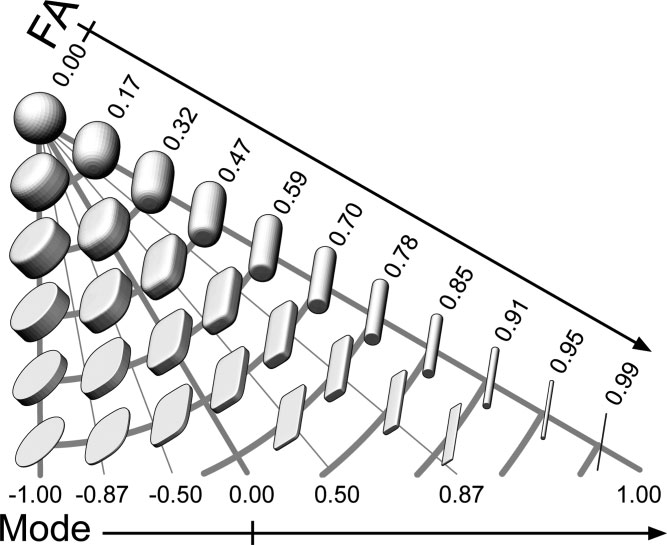
\includegraphics[width=0.5\textwidth]{pictures/001.png}
	\caption{Darstellung der fraktionalen Anisotropie und des Modus von Matrizen in Form von Superquadrics\cite{kindlmann2004superquadric}. Die fraktionale Anisotropie nimmt mit gr\"o{\ss}er werdender Entfernung zum obersten linken Superquadric zu. Der Modus des Deviators wird abh\"angig vom Winkel dargestellt, wobei er links -1 betr\"agt und rechts 1. Entnommen aus \cite[S.~140]{ennis2006orthogonal}.}
	\label{Modus}
\end{figure}
Um die Intuition hinter Modus und fraktionaler Anisotropie zu verdeutlichen, sind in \cref{Modus} Superquadrics von Matrizen unterschiedlicher Modi dargestellt. Insbesondere soll damit gezeigt werden, dass der Modus nicht von der Gr\"o{\ss}e der Eigenwerte abh\"angt, sondern von deren Verteilung.

\subsubsection{Gradient}
Der Gradient einer skalaren Funktion $f: \mathbb{R}^n \rightarrow \mathbb{R}$  \"uber einem kartesischen Koordinatensystem ist definiert als

\begin{equation}
	grad(f) = 	
	\begin{pmatrix}
		\frac{\partial f}{\partial x_1} \\
		\vdots \\
		\frac{\partial f}{\partial x_n}
	\end{pmatrix},
\end{equation}

also als Vektor aller partiellen Ableitungen in die Richtungen $x_i$. Analog ist der Gradient einer Skalarfunktion $g: K^{m\times n} \rightarrow \mathbb{R}$, wobei $K^{m\times n}$ der Raum aller $m\times n$ Matrizen ist, definiert als

\begin{equation}
	grad(g) =
	\begin{pmatrix}
		\frac{\partial f}{\partial a_{11}} & \dots & \frac{\partial f}{\partial a_{1n}}  \\
		\vdots & \ddots & \vdots \\
		\frac{\partial f}{\partial a_{m1}} & \dots & \frac{\partial f}{\partial a_{mn}} 
	\end{pmatrix},
\end{equation}

wobei $a_{ij}$ die Komponenten der Matrizen sind.

\subsubsection{Orthogonalit\"at von Matrizen}
Zwei Matrizen $U,V$ werden als orthogonal zueinander bezeichnet, wenn \cite{ennis2006orthogonal} gilt:

\begin{equation}
tr(U,V^{T}) = 0
\end{equation}

\subsubsection{Matrixinvarianten}
\label{Matrixinvarianten}
Als Invarianten werden zu mathematischen Objekten zugeordnete Gr\"o{\ss}en bezeichnet, die invariant gegen\"uber der Anwendung bestimmter Transformationen auf die Objekte sind. Invarianten eines Tensors in Matrixdarstellung, im Folgenden kurz Invarianten genannt, sind beispielsweise Gr\"o{\ss}en, die sich unabh\"angig von der Wahl der Basis der Matrix nicht ver\"andern\cite{ennis2006orthogonal}. Eine Invariante ist somit eine Funktion $\Psi: M \rightarrow A$ die Objekten aus dem Vektorraum aller Matrizen $M$ Objekte aus der Menge $A$ zuordnet. In der Praxis wird f\"ur $A$ meistens $\mathbb{R}$ gew\"ahlt.

Da sich die vorliegende Arbeit \"uberwiegend mit symmetrischen, dreidimensionalen Tensoren zweiten Grades und ausschlie{\ss}lich mit orthogonalen Transformationen besch\"aftigt, beschr\"ankt sich auch die Betrachtung der Invarianten im Folgenden auf diese Art von Tensoren. Dabei gilt f\"ur solche Tensoren insbesondere, dass die Invarianten eines Tensors $T$ durch seine Eigenwerte vollst\"andig charakterisiert werden. Invarianten sind in diesem Spezialfall also auch als Funktion $\Psi: \mathbb{R}^d \rightarrow \mathbb{R}$ der Form

\begin{equation}
	\Psi:
	\begin{bmatrix}
	\lambda_1\\
	\lambda_2\\
	\lambda_3
	\end{bmatrix}
	\rightarrow \mathbb{R}
\end{equation}

darstellbar, wobei $\lambda_1, \lambda_2, \lambda_3$ die Eigenwerte von $T$ sind. Dies stimmt mit der Betrachtunsweise von Zobel und Scheuermann \cite{zobel2017extremal} \"uberein.

\subsubsection{Invariantens\"atze} 
\label{sec:Invariants}
Mengen von Invarianten werden als Invariantens\"atze bezeichnet.
Matrixinvarianten $\Psi_1$ und $\Psi_2$ werden als orthogonal zueinander bezeichnet, wenn ihre Gradienten f\"ur jede m\"ogliche Eingabematrix orthogonal sind. Die genauen Definitionen und Berechnungen dazu sind in den Arbeiten von Ennis, Kindlmann et al. \cite{ennis2006orthogonal} nachzulesen. Da Gradienten von skalarwertigen Funktionen auf Matrizen wiederum Matrizen sind \cite[S.~137]{ennis2006orthogonal}, gen\"ugt es zu zeigen, dass diese orthogonal zueinander sind. Invariantens\"atze, deren Elemente paarweise orthogonal sind, werden als orthogonale Invariantens\"atze bezeichnet.

F\"ur $3\times 3$ Matrizen enthalten alle orthogonalen Invariantens\"atze h\"ochstens drei Invarianten. In der Praxis spielt eine Vielzahl solcher Invariantens\"atze eine Rolle, von denen im Folgenden einige erl\"autert werden.

Wenn die zu einem Invariantensatz geh\"orenden Invarianten einer Matrix $M$ berechnet wurden, so stellen diese eine Repr\"asentation der basisunabh\"angigen Eigenschaften von $M$ dar. In dieser Arbeit wurden ausschlie{\ss}lich symmetrischen $3\times3$ Matrizen visualisiert, die aus bis zu 6 nicht-doppelten Werten bestehen k\"onnen. Die Beschreibung dieser 6 Werte durch die 3 Invarianten ist nicht ohne Informationsverlust m\"oglich. Die verlorenen 3 Werte an Information sind jedoch ausschlie{\ss}lich Informationen \"uber die Richtung der Eigenvektoren, was in vielen Anwendungsf\"allen nicht von Interesse ist.

Welcher der Invariantens\"atze f\"ur einen bestimmten Datensatz verwendet wird, kann abh\"angig von der Dom\"ane ausgesucht werden. Die Wahl ist nat\"urlich abh\"angig von den schon genannten Interpretationen der Invarianten in den jeweiligen Dom\"anen.

\paragraph{Die Eigenwerte}

Die Eigenwerte bilden einen orthogonalen Invariantensatz. Sie sind insbesondere in der Medizin sehr beliebt, da hohe Eigenwerte von Diffusionstensoren auf die Bewegungsrichtung von Molek\"ulen in Gewebe schlie{\ss}en lassen.

\paragraph{Der I-Invariantensatz}
Das charakteristische Polynom $\chi$ einer $3\times3$ Matrix $A$ hat die Form

\begin{equation}
	\centering
	\begin{split}
	&\chi_A(a) = det(a \cdot I - A)\\
	&\chi_A(a) = -a^3 + I_1\cdot a^2 - I_2\cdot a + I_3,
	\end{split}
\end{equation}

wobei $\lambda$ ein Element aus dem K\"orper von $A$ und $I$ die dreidimensionale Einheitsmatrix ist. Es wird h\"aufig verwendet, um die Eigenwerte von Matrizen zu bestimmen, da diese den Nullstellen des Polynoms entsprechen.

Eine weitere Eigenschaft ist, dass die Parameter $I_1, I_2, I_3$ einen Invariantensatz darstellen. Wegen der Wichtigkeit des charakteristischen Polynoms werden sie h\"aufig als \glq Hauptinvarianten\grq{} bezeichnet. Alternativ k\"onnen sie auch berechnet werden als

\begin{itemize}
	\item $I_1(A) = tr(A)$ (Spur von $A$)
	\item $I_2(A) = \frac{1}{2}(tr(A)^2 - tr(A^2))$ (Summe der Hauptminoren von $A$)
	\item $I_3(A) = det(A)$ (Determinante von $A$)
\end{itemize}

Der I-Invariantensatz ist jedoch nicht orthogonal. Die Beweise oder Wiederlegungen der Orthogonalit\"atseigenschaft aller hier vorgestellter Invariantens\"atze sind in \cite[S.~144]{ennis2006orthogonal} aufgef\"uhrt.

W\"ahrend in der Mechanik f\"ur $I_1$ eine Interpretation als Ma{\ss} f\"ur den isotropen Anteil des Tensors existiert, fehlen eindeutige Interpretationen f\"ur $I_2$ und $I_3$. Es gibt zwar einen Zusammenhang zwischen $I_2$ und dem deviatorischen Anteil des Tensors, dieser ist jedoch nicht eindeutig genug um aus hohem $I_2$ auf hohe Anisotropie schlie{\ss}en zu k\"onnen. F\"ur $I_3$ existiert in der Mechanik keine verbreitete Interpretation. 

\paragraph{Der J-Invariantensatz}

Die Berechnung der J-Invarianten ist identisch zum I-Invarian\-ten\-satz, nur dass statt $A$ der Deviator von $A$ als Eingabe verwendet wird:

\begin{itemize}
	\item $J_1(A) = tr(\tilde{A})$ (Spur des Deviators von $A$)
	\item $J_2(A) = \frac{1}{2}(tr(\tilde{A})^2 - tr(\tilde{A}^2))$ (Summe der Hauptminoren des Deviators von $A$)
\item $J_3(A) = det(\tilde{A})$ (Determinante des Deviators von $A$)
\end{itemize}

Dabei ist jedoch zu beachten, dass

\begin{equation}
	\begin{split}
	tr(\tilde{A}) &= tr(A - \frac{1}{3}tr(A)I)\\
	&= a_{11} - \frac{1}{3} tr(A) + a_{22} - \frac{1}{3} tr(A) + a_{33} - \frac{1}{3} tr(A)\\
	&= a_{11} + a_{22} + a_{33} - tr(A)\\
	&= tr(A) - tr(A)\\
	&= 0,
	\end{split}
\end{equation}

weshalb statt $J_1$ in der Regel $I_1$ als Teil des Invariantensatzes verwendet wird. \"Ahnlich wie I ist auch J nicht orthogonal.

\paragraph{Der K-Invariantensatz}
Der K-Invariantensatz ist orthogonal und ist f\"ur eine Matrix $A$ definiert als

\begin{itemize}
	\item $K_1(A)=tr(A)$ (Spur von $A$)
	\item $K_2(A)=norm(\tilde{A})$ (Norm des Deviators von A)
	\item $K_3(A)=mode(\tilde{A})$ (Modus des Deviators von A).
\end{itemize}


\begin{figure}
	\centering
	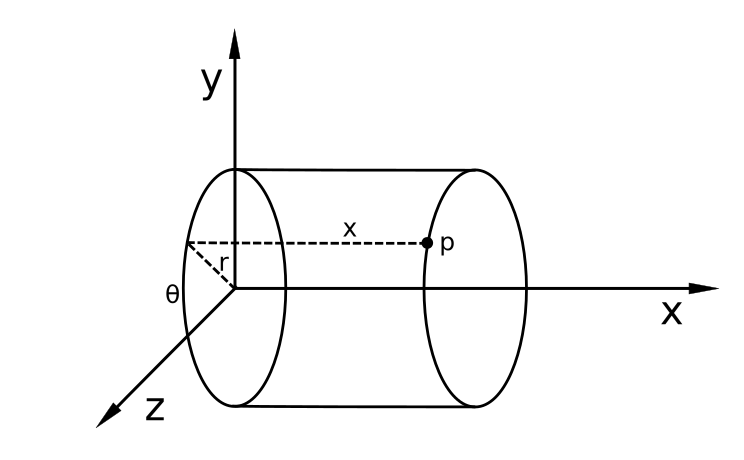
\includegraphics[width=0.5\textwidth]{pictures/cylinder}
	\caption{Darstellung eines zylindrischen Koordinatensystems. $x,y$ und $z$ entsprechen dabei den kartesischen Achsen. Die Koordinaten des Punktes $p$ sind angegeben als $x, r, \theta$. $x$ entspricht der kartesischen Koordinate, $r$ ist die Entfernung zwischen der Projektion von $p$ auf die von $y$ und $z$ Achse aufgespannte Fl\"ache und dem Koordinatenursprung und $\theta$ entspricht dem Winkel zwischen Projektion von $p$, dem Koordinatenursprung und der x-Achse. }
	\label{cylinderCoords}
\end{figure}

Da $K_1 \in [-\infty; \infty]$, $K_2 \in [0;\infty]$ und $K_3 \in [-1;1]$ ist, bietet sich f\"ur den K-Invariantensatz eine Darstellung in einem zylindrischen Koordinatensystem an, wobei $K_1$ eine Position auf einer zentralen Achse beschreibt, $K_2$ die orthogonale Entfernung zu diesem Punkt und $K_3$ den Winkel zu einer festgelegten, zur zentralen Achse orthogonalen, zweiten Achse. Sowohl ein zylindrisches als auch ein kartesisches Koordinatensystem sind in \cref{cylinderCoords} dargestellt. $K_1$ entspricht dabei der zylindrischen $x$-Koordinate, $K_2$ dem Radius $r$ und $K_3$ dem Winkel $\theta$.

Ein Vorteil des K-Invariantensatzes ist die relativ leichte Interpretierbarkeit in der Kontinuumsmechanik. $K_1$ kann als Ma{\ss} der St\"arke des iostropen Anteils der Matrix, $K_2$ als Ma{\ss} des anisotropen Anteils angesehen werden \cite{kindlmann2007diffusion}. Dagegen kann aus dem Wert von $K_3$ die Verteilung der Eigenwerte und damit die Form der Anisotropie des Tensors geschlussfolgert werden.



\paragraph{Der R-Invariantensatz}
Die Invarianten des orthogonale R-Invariantensatz sind f\"ur eine Matrix $A$ definiert als

\begin{itemize}
	\item $R_1(A)=norm(A)$ (Norm von $A$)
	\item $R_2(A)=\sqrt{\frac{3}{2}} \frac{norm(\tilde{A})}{norm(A)}$ (fraktionale Anisotropie)
	\item $R_3(A)=mode(A)$ (Modus von $A$).
\end{itemize}

Dabei f\"allt auf, dass gilt $R_3(A) = K_3(A) = mode(A)$. \"Ahnlich wie der K-Invariantensatz k\"onnen auch die R-Invarianten in einem zylindrischen Koordinatensystem dargestellt werden.

\begin{figure}
	\centering
	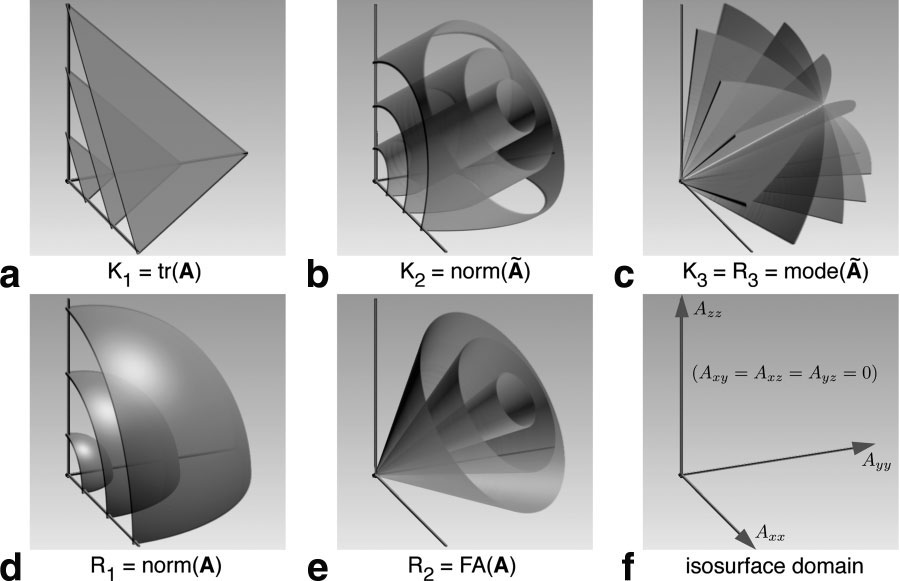
\includegraphics[width=0.5\textwidth]{pictures/000.png}
	\caption{Dargestellt sind Isofl\"achen der K- und R-Invarianten von diagonalisierten $3\times 3$ Matrizen (alle Werte au{\ss}erhalb der Hauptdiagonale sind 0). Die Koordinatenachsen entsprechen den drei Eigenwerten der Matrizen. Entnommen aus \cite[S.~139]{ennis2006orthogonal}}
	\label{KRInvariants}
\end{figure}

Genauso wie f\"ur den K-Invariantensatz existiert auch f\"ur den R-Invariantensatz eine Interpretation in der Kontinuumsmechanik. 

Sowohl K- als auch R-Invarianten beschreiben die Verteilung, die \glq Gr\"o{\ss}e\grq{} und das Verh\"altnis der Eigenwerte zueinander. Dies ist in \cref{KRInvariants} dargestellt.

\subsubsection{Kontinuierliche Menge}
\subsubsection{Diskrete Menge} 

\subsubsection{Faltung}
Die kontinuierliche Faltung $*_c$ zweier Funktionen $f,g:\mathbb{R}^n\rightarrow\mathbb{C}$ ist definiert als

\begin{equation}
(f*_cg)(x) = \int_{\mathbb{R}^n} f(\tau)g(x-\tau)d\tau.
\end{equation}

Falls das Urbild beider Funktionen eine diskrete Menge $\mathbb{D} \subset \mathbb{R}^n$ ist, wird stattdessen die diskrete Faltung $*_d$ verwendet. Diese ist definiert als

\begin{equation}
(f*_dg)(n) = \sum_{k\in\mathbb{D}}f(k)g(n-k).
\end{equation}

Das Ergebnis der Faltung ist eine neue Funktion, die bildlich betrachtet den um $g$ gewichteten Mittelwert von $f$ an jedem Punkt darstellt. $g$ wird in diesem Fall als Kern oder Faltungskern bezeichnet. Um beispielsweise den Wert von $(f*g)$ an der Stelle $x$ zu bestimmen, wird $g$ um $x$ verschoben, $f$ und $g$ punktweise multipliziert und das Integral des Ergebnisses gebildet, was der Bestimmung des Mittelwerts entspricht. Dies geht aus dem Mittelwertsatz der Integralrechnung hervor.

\subsubsection{Gau{\ss}sche Glockenkurve}
Glockenkurven sind Funktionen der Form 

\begin{equation}
f(x) = \frac{1}{\sqrt{2\pi \sigma^2}}e^{-\frac{(x-\mu)^2}{2\sigma^2}}.
\end{equation}

Die Variablen $\mu$ und $\sigma$ dienen dazu, die Form der Glockenkurve und ihre Position im Koordinatensystem zu beeinflussen. Das Maximum der Glockenkurve liegt immer bei $\mu$. Mit $\sigma$ l\"asst sich die Breite und H\"ohe der Glockenkurve beeinflussen, wobei die Fl\"ache darunter gleich bleibt.

In \cref{Gauss} sind drei Glockenkurven mit unterschiedlichen Werten f\"ur $\mu$ und $\sigma$ dargestellt.

\pgfmathdeclarefunction{gauss}{2}{%
	\pgfmathparse{1/(#2*sqrt(2*pi))*exp(-((x-#1)^2)/(2*#2^2))}%
}

\begin{figure}
	\centering
	\begin{tikzpicture}
	\begin{axis}[
	no markers, domain=0:10, range=0:10, samples=100,
	axis x line=left,
	axis y line=middle,
	xlabel=$x$, ylabel=$y$,
	every axis y label/.style={at=(current axis.above origin),anchor=south},
	every axis x label/.style={at=(current axis.right of origin),anchor=west},
	height=5cm, width=8cm,
	xtick={1,2,3,4,5,6,7,8,9,10}, 
	ytick={0.1,0.2,0.3,0.4,0.5,0.6,0.7,0.8,0.9,1.0},
	yticklabels={{0,1},{0,2},{0,3},{0,4},{0,5},{0,6},{0,7},{0,8},{0,9},{1,0}},
	enlargelimits=false, clip=false, axis on top,
	grid = major
	]
	\addplot [very thick,red] {gauss(5,2 )};
	\addplot [very thick,green] {gauss(6,1 )};
	\addplot [very thick,blue] {gauss(7,0.5 )};
	\end{axis}
	
	\end{tikzpicture}
	\caption{Darstellung von drei Gau{\ss}schen Glockenkurven mit unterschiedlichen $\mu$ und $\sigma$: Rot: $\mu=5, \sigma=2$, Gr\"un: $\mu=6, \sigma=1$, Blau: $\mu=7, \sigma=$0,5}
	\label{Gauss}
\end{figure}

Im zweidimensionalen Fall existieren analoge Glockenkurven der Form

\begin{equation}
	f(x,y) = 
	\frac{1}{\sqrt{2\pi \sigma_x^2}}e^{-\frac{(x-\mu_x)^2}{2\sigma_x^2}} \cdot 
	\frac{1}{\sqrt{2\pi \sigma_y^2}}e^{-\frac{(x-\mu_y)^2}{2\sigma_y^2}}.
\end{equation}

Die Variablen $\mu_x$ und $\mu_y$ dienen dabei dazu, die Positionen der Kurven in der jeweiligen Dimension festzulegen. Die H\"ohe und Form der Glockenkurve ergeben sich aus $\sigma_x$ und $\sigma_y$. Eine Erh\"ohung von $\sigma_x$ beispielsweise f\"uhrt dazu, dass die H\"ohe des Extremums reduziert und die Glocke in x-Richtung gestreckt wird.

\subsection{Mechanische Grundlagen}
\subsubsection{Physikalisches Feld}
Ein physikalisches Feld ist eine physikalische Gr\"o{\ss}e, die an verschiedenen Positionen im Raum unterschiedliche Werte annimmt\cite[1–2 Electric and magnetic fields]{feynman2011feynman}. Abstrahiert kann es als Funktion $\mathbb{R}^n \rightarrow V$ beschrieben werden, wobei $V$ eine beliebige Menge ist. H\"aufig wird f\"ur $V$ jedoch $\mathbb{R}$, z.B. bei Temperaturen, $\mathbb{R}^n$, z.B. bei Str\"omungen, oder $\mathbb{R}^{m\times n}$, z.B. bei Verformungen, eingesetzt. Andere Beispiele f\"ur physikalische Felder sind elektromagnetische Felder oder Gravitationsfelder. Felder werden meist abh\"angig von ihrem Bild klassifiziert, so z.B. in Skalar-, Vektor- oder Tensorfelder.

Wenn Felder nicht in Form einer kontinuierlichen Funktion beschrieben werden k\"onnen, weil z.B. nur f\"ur endlich viele Punkte Messwerte vorhanden sind, kann ein Feld auf einem Gitter, das aus diesen Messpunkten besteht, definiert werden. Die Werte innerhalb der Zellen lassen sich dann durch Interpolation der Werte an den Eckpunkten berechnen.


Innerhalb der vorliegenden Arbeit werden Spannung und Verformung an Punkten von Objekten als Felder $\mathbb{R}^3 \rightarrow \mathbb{R}^{m\times n}$ beschrieben.


\subsubsection{Mechanische Spannung}
In der Mechanik beschreibt Spannung die Kr\"afte, die Partikel innerhalb eines Objektes aufeinander auswirken. Um die Spannung an einem Punkt zu bestimmen, wird die Kraft, die auf infinitesimal kleine Fl\"achenteile von Schnitten durch das Objekt wirkt, berechnet. Die Kraft ist dabei als Vektor formulierbar. Wenn die Schnitte entlang von drei zueinander orthogonalen Ebenen durchgef\"uhrt werden, erh\"alt man so drei Vektoren, die zusammen die Matrixdarstellung des Cauchy Tensors $\sigma$ bilden:

\begin{equation}
	\sigma =  
	\begin{bmatrix}
		\sigma_x & \tau_{xy} & \tau_{xz}\\
		\tau_{xy} & \sigma_y & \tau_{yz}\\
		\tau_{xz} & \tau_{yz} & \sigma_z
	\end{bmatrix}
\end{equation}

Jede Spalte des Cauchy Tensors entspricht dabei einem der Vektoren. Wie aus der Formel ersichtlich, ist die Matrix symmetrisch und enth\"alt zwei Typen von Komponenten: Die $\sigma$ entlang der Hauptdiagonale, die Kraft in Richtung der Normalen der jeweiligen Ebene angeben, und den $\tau$, die Scherspannungen angeben, die parallel zu den Schnittebenen verlaufen. 

\subsubsection{Mechanische Verformung}
Wenn in einem Objekt Spannung vorliegt, so verformt es sich proportional zur St\"arke der Spannung (Hookesches Gesetz). Durch einen Verformungstensor, auch Verzerrungstensor gennant, l\"asst sich die Verformung an einem Punkt durch Kraftanwendung angeben:

\begin{equation}
	\epsilon  =  
	\begin{bmatrix}
		\epsilon_x & \frac{1}{2}\gamma_{xy} & \frac{1}{2}\gamma_{xz}\\
		\frac{1}{2}\gamma_{xy} & \epsilon_y & \frac{1}{2}\gamma_{yz}\\
		\frac{1}{2}\gamma_{xz} & \frac{1}{2}\gamma_{yz} & \epsilon_z
	\end{bmatrix}
\end{equation}

\"Ahnlich wie beim Spannungstensor dr\"ucken die $\epsilon$ in der Hauptdiagonale Dehnungen oder Stauchungen des Objektes entlang der Hauptachsen aus, die $\gamma$ Werte Scherungen, also Verschiebungen der Seitenfl\"achen zueinander. Dabei \"andern sich die Winkel der Kanten des Objektes zueinander.

\section{Verwendete Verfahren und Technologien}
\label{sec:Technologien}
\subsection{FAnToM}
FAnToM\cite{fantomWebsite,wiebel2009fantom} (\glqq Field Analysis using Topological Methods\grqq{}) ist ein Programm, dessen Entwicklung im Jahre 1999 begann. Obwohl es zu Anfang noch als Hilfsmittel f\"ur die Analyse von Vektorfeldtopologien konzipiert war, entwickelte es sich \"uber die Jahre hinweg zu einer Plattform f\"ur diverse Visualisierungen.

Erweiterungen von FAnToM werden in Form von sogenannten \glq Algorithmen\grq{} entwickelt. Dabei unterscheidet man zwei Arten: den \glq Data Algorithmus\grq{} und den \glq Visualization Algorithmus\grq{}. Data Algorithmen sind Erweiterungen, die Daten verarbeiten. Beispiele daf\"ur sind \glq Load VTK\grq{}, eine Erweiterung, die Daten aus dem VTK Format einliest, oder \glq Combine Scalar to Vector\grq{}, das mehrere Felder mit skalaren Werten zu einem einzigen Feld mit Vektorwerten kombiniert, wobei die Komponenten eines Vektors an einem Punkt den Skalaren der Eingabefelder am selben Punkt entsprechen.
Visualization Algorithmen dagegen dienen dazu, Visualisierungen aus Daten zu erzeugen. Interaktionen mit den Visualisierungen k\"onnen entweder \"uber die Maus oder \"uber Optionen stattfinden. Ein Beispiel f\"ur einen Visualization Algorithmus ist \glq Show Grid\grq{}, durch das eine Zellstruktur als Gitternetz dargestellt word

Ein wesentliches Feature von FAnToM besteht darin, Algorithmen miteinander zu verkn\"upfen. Dies geschieht, indem Ausgabedaten von Algorithmen als Eingabe f\"ur andere dienen k\"onnen. Da viele Algorithmen mit Blick auf Wiederverwendbarkeit entwickelt wurden, k\"onnen mit wenig Aufwand aus bestehenden Algorithmen komplett neue Visualisierungspipelines entwickelt werden. Dies geschieht mittels des sogenannten \glq Flow Graphs\grq{}, in dem Algorithmen als Knoten dargestellt sind, deren Aus- und Eingaben miteinander verbunden werden k\"onnen, was als Verbindung zwischen den jeweiligen Knoten im Flow Graph dargestellt wird.

Diese Pipelines k\"onnen als FAnToM-Session abgespeichert und sp\"ater wiederhergestellt werden.

FAnToM bietet eine Vielzahl m\"achtiger Werkzeuge, auf die bei der Entwicklung neuer Erweiterungen zur\"uckgegriffen werden kann. Besonders relevant f\"ur die vorliegende Arbeit waren dabei Funktionen zur effizienten Verarbeitung von Feldern und Tensoren, die Schnittstellen f\"ur Qt und OpenGL sowie die gro{\ss}e Bibliothek bestehender Algorithmen.

\subsection{OpenGL}
\label{sec:OpenGL}
OpenGL\cite{openglWebsite} ist eine Spezifikation, die das Verhalten eines rasterbasierten Renderingsystems beschreibt. Sie definiert eine Schnittstelle, gegen die von zwei Seiten entwickelt werden kann: Zum einen von Seiten der Hardwarehersteller, die Funktionen von OpenGL auf ihrer Hardware implementieren, zum anderen von Anwendungsprogrammierern, die unabh\"angig von der Hardware, auf der das Programm laufen soll, gegen die Spezifikation von OpenGL entwickeln k\"onnen. Da in der vorliegenden Arbeit OpenGL nur aus Sicht eines Anwendungsprogrammierers verwendet wurde, beschr\"ankt sich die folgende Beschreibung darauf.

Die Verarbeitungsschritte von der \"Ubergabe von Daten aus einer Anwendung zu OpenGL bis zum fertig gerenderten Bild werden als Renderpipeline bezeichnet. Seit Version 2.0 unterst\"utzt OpenGL sogenannte \glq Shader\grq{}, kleine Programmst\"ucke, die es Nutzern von OpenGL erm\"oglichen, die Renderpipeline sehr stark zu ver\"andern. Shader bekommen drei Arten von Eingabedaten:

\begin{enumerate}
	\item Die Ausgabe des vorherigen Schrittes in der Renderpipeline
	\item Parameter aus dem Programm, das OpenGL verwendet (\glq Uniforms\grq{})
	\item Daten, die aus dem vorhergehenden Shader \"ubergeben wurden
\end{enumerate}

Ein wichtiger Spezialfall von Uniforms sind Texturen, die in dem OpenGL verwendenden Programm geladen, an die Shader \"ubergeben und dort verwendet werden k\"onnen.

F\"ur die vorliegende Arbeit wurden Vertex, Geometry und Fragment-Shader entwickelt. Diese drei Typen sind im Folgenden kurz erkl\"art.

\paragraph{Vertex-Shader}
Vertex-Shader bekommen als Eingabe aus der Renderpipeline die Punkte eines zu zeichnenden Grafik-Primitive, beispielsweise die Punkte eines Liniensegmentes oder die Eckpunkte eines Dreiecks. Abh\"angig von den eingegebenen Uniforms k\"onnen die Koordinaten dieser Punkte dann durch den Shader ver\"andert werden. Dies ist z.B. \"ublich, um die Sicht auf die Szene von der Position red Kamera aus zu berechnen. Vertex-Shader werden einmal pro Punkt ausgef\"uhrt. Die Ausgabe des Vertex-Shaders sind die neuen Koordinaten der Punkte der Primitives.

\paragraph{Geometry-Shader}
Die Renderpipeline \"ubergibt dem Geometry-Shader f\"ur jedes Primitive eine Liste der zugeh\"origen Punkte, z.B. eine Liste von drei Punkten f\"ur ein Dreieck. Der Geometry-Shader ist in der Lage, die Position und den Typ dieser Primitives beliebig zu ver\"andern und sogar neue Punkte zu erzeugen. So kann er beispielsweise aus einer Linie ein Dreieck erzeugen, sowie Uniforms pro Punkt definieren, welche an sp\"ater ausgef\"uhrte Shader (z.B. den Fragment-Shader) weitergegeben werden. Pro Primitive wird der Geometry-Shader einmal ausgef\"uhrt.

\paragraph{Fragment-Shader}
Fragment-Shader bestimmen die Farben der Fragmente. Fragmente sind St\"ucke der projizierten Primitives, deren Gr\"o{\ss}e von der Art der Rasterisierung abh\"angen. Aus den Fragmenten werden die Farben der Pixel des gerenderten Bildes bestimmt. In der Regel wird pro Pixel mindestens ein Fragment berechnet. Wenn mehrere Fragmente zu einem Pixel kombiniert werden bezeichnet man dies als Supersampling. Die Eingaben in den Fragment-Shader sind die Mittelpunkte der Fragmente und die f\"ur diese Punkte interpolierten Attribute der Eckpunkte des Primitive. Neben der Fragmentfarbe k\"onnen auch andere Werte berechnet und ausgegeben werden, z.B. ein Tiefenattribut, das die Entfernung des Fragments zur Kamera angibt und damit korrekte \"Uberlappung von Primitives erm\"oglicht.

Eine weitere im Folgenden verwendete Funktion von OpenGL ist die M\"oglichkeit, gerenderte Bilder mithilfe von \glq Framebuffern\grq{} nicht anzuzeigen, sondern stattdessen in einer Textur zu speichern. Diese abgelegten Bilder k\"onnen durch das sogenannte \glq Blending\grq{} mit den Ergebnissen sp\"aterer Renderings kombiniert werden. Dabei wird ein weiteres Bild auf dem bestehenden gezeichnet und die Farbwerte entsprechend von Wichtungsfunktionen kombiniert. Dies erm\"oglicht beispielsweise die Darstellung transparenter Objekte.

Die meisten Implementierungen von OpenGL machen intensiven Gebrauch von Grafikkarten und deren F\"ahigkeit zur extremen Parallelisierung von Aufgaben. Dies, verbunden mit der M\"oglichkeit Ausgaben der Renderpipeline zur\"uck in den Arbeitsspeicher zu laden und der Anpassbarkeit der Renderpipeline durch Shader, erm\"oglicht es, OpenGL generell f\"ur rechenintensive, gut parallelisierbare Aufgaben zu benutzen und so Berechnungen stark zu beschleunigen.

\subsection{Qt}
Qt\cite{qtWebsite} ist eine popul\"are, plattform\"ubergreifende Bibliothek f\"ur die Entwicklung von Programmoberfl\"achen. Die Popularit\"at von Qt beruht auf der Plattformunabh\"angigkeit und der gro{\ss}en Vielfalt leicht zu verwendender Funktionen. Darunter sind beliebte Oberfl\"achenelemente wie Kn\"opfe, Textfelder und Ankreuzk\"asten, wodurch die Gestaltung einer Nutzerschnittstelle sehr einfach wird.

FAnToM besitzt eine auf Qt basierende Oberfl\"ache, die aus Algorithmen heraus um weitere Fenster und Elemente erweitert werden kann. Eine wesentliche F\"ahigkeit von Qt ist dabei, einen OpenGL Kontext zu erzeugen, sodass durch OpenGL gerenderte Bilder angezeigt werden k\"onnen. Diese F\"ahigkeit von Qt wird innerhalb dieser Arbeit verwendet, um mehrere, unabh\"angige Datensichten zu implementieren. 

\subsection{Continuous Scatterplotting}
\subsubsection{Scatterplotting}
\begin{figure}
	\hspace{2cm}
	\begin{subfigure}{0.30\textwidth}
		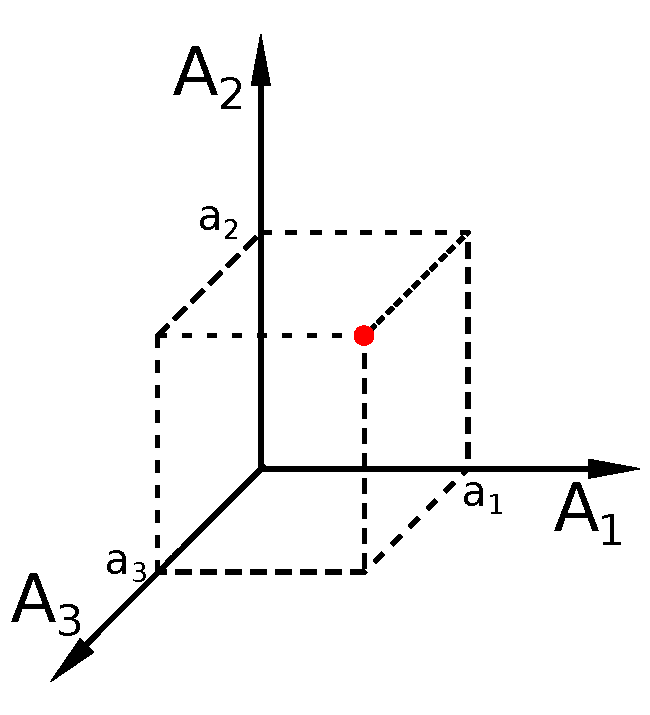
\includegraphics[width=\textwidth]{pictures/Scatterplot3D}
		\caption{}
	\end{subfigure}
	\hfill
	\begin{subfigure}{0.30\textwidth}
		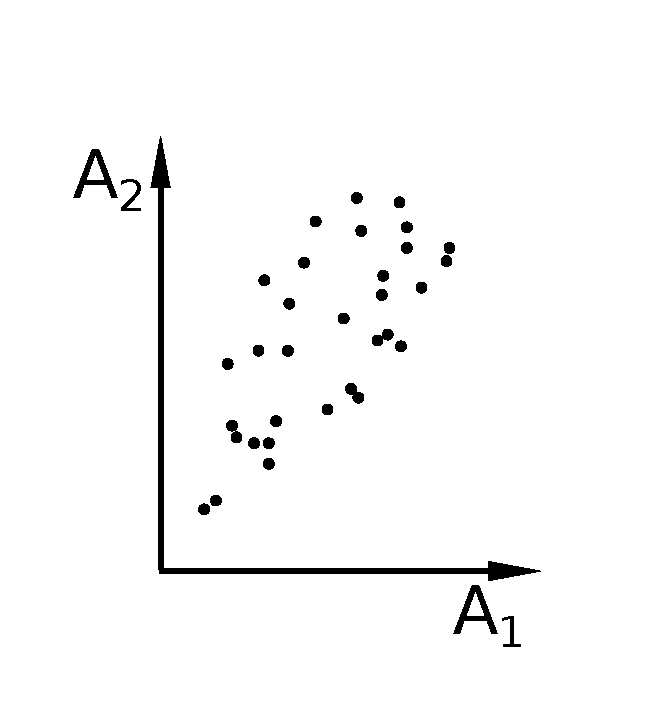
\includegraphics[width=\textwidth]{pictures/Scatterplot2D}
		\caption{}
	\end{subfigure}
	\hspace{2cm}
	\caption{Zwei Beispiele f\"ur Scatterplottings. In (a) wird ein Objekt mit den Attributwerten $a_1, a_2, a_3$ als roter Punkt iKCSGK6Q8rBsihln einem dreidimensionalen Scatterplot dargestellt. Um die Attribute besser ablesen zu k\"onnen, wurden gestrichelte Linien eingezeichnet. In (b) wurden mehrere Objekte mit unterschiedlichen Attributen im selben, zweidimensionalen Scatterplot als schwarze Punkte eingezeichnet.}
	\label{Scatterplots}
\end{figure}

Scatterplotting ist ein weit verbreitetes Verfahren, um Attribute von Objekten in Relation zueinander darzustellen. Es ist eine Funktion auf einer Menge von Objekten $M$ als $\tau: M \rightarrow \mathbb{R}^n,n\in\{1,2,3\}$, wobei das Bild eine Projektion auf einzelne oder zusammengesetzte Attribute der Objekte darstellt.  Dazu wird je Objekt ein Punkt in ein ein-, zwei- oder dreidimensionales Koordinatensystem eingetragen, dessen Koordinatenachsen Attributwerten entsprechen. Beispiele f\"ur Scatterplottings sind in \cref{Scatterplots} zu sehen. Das Bild von $\tau$ ist auf maximal drei Dimensionen beschr\"ankt, da h\"oherdimensionale Daten visuell nur schwer zu interpretieren sind.

Ein Vorteil von Scatterplottings ist die leichte Erkennbarkeit von Strukturen in den Datens\"atzen: Bereiche hoher Punktdichte (Cluster), Punkte weit entfernt von allen anderen Punkten (Outlier) und funktionale Zusammenh\"ange zwischen den verwendeten Attributen lassen sich gut identifizieren. 

Scatterplotting hat jedoch zwei gravierende Nachteile. Zum einen macht die geringe Dimensionalit\"at des Bildes von $\tau$ oft die Projektion auf eine Teilmenge der Attribute der dargestellten Objekte notwendig, zum anderen kann Scatterplotting nur endlich viele Objekte gleichzeitig darstellen.

Ein praktisches Beispiel eines Urbildes mit unendlich vielen Elementen ist $\mathbb{R}^n$ bei physikalischen Feldern. Dort sind an jedem der unendlich vielen Punkte im Raum Werte definiert. Ein Scatterplot dieser unendlich vielen Elemente ist nun weder in endlicher Laufzeit m\"oglich, noch w\"aren einzelne Punkte in der entstehenden Darstellung erkennbar, da in jedem Fall nur endlich viele Pixel zur Verf\"ugung stehen. Eine Alternative besteht darin, nur den Scatterplot der Eckpunkte der Zellen zu erzeugen, doch damit gehen Informationen \"uber das Innere der Zellen verloren.


\subsubsection{Erkl\"arung des Continuous Scatterplotting}
\begin{figure}
	\centering
	\begin{subfigure}{0.45\textwidth}
		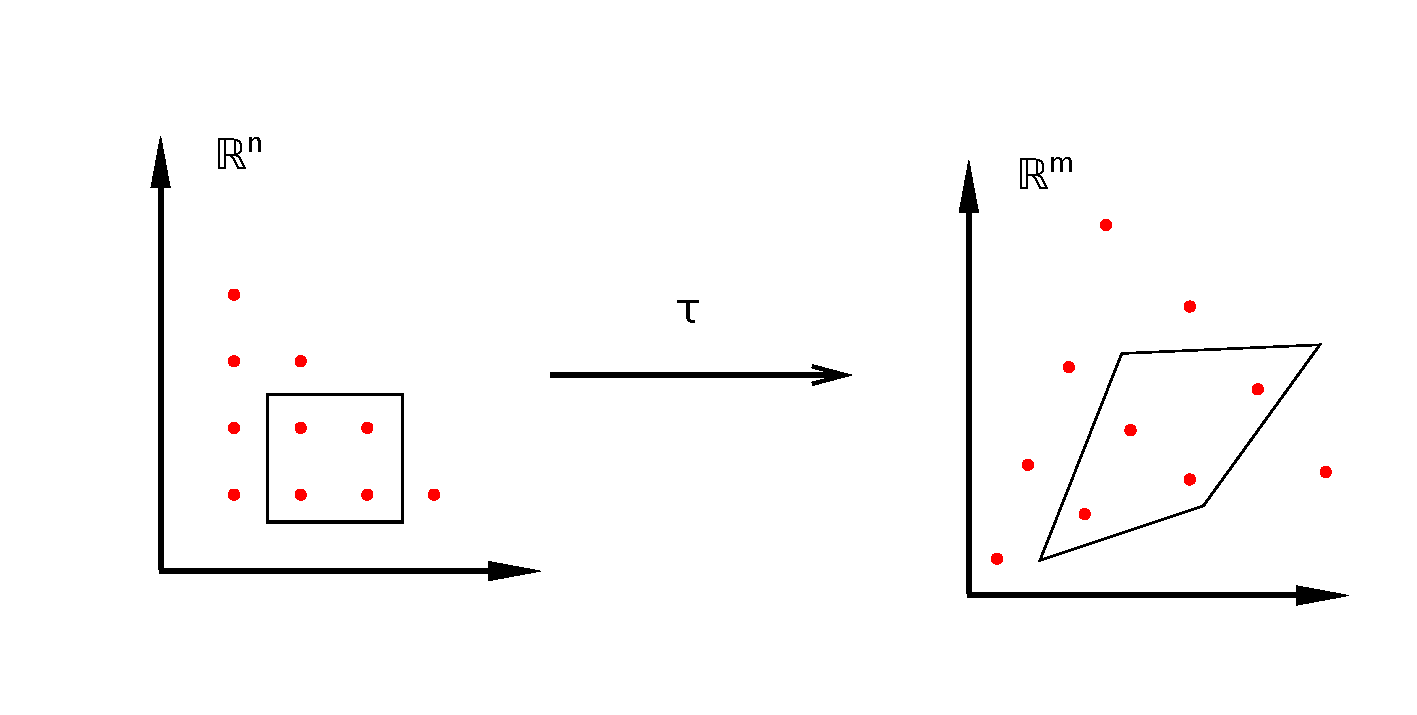
\includegraphics[width=0.9\textwidth]{pictures/ContinuousScatterplot}
		\subcaption{}
	\end{subfigure}
	\begin{subfigure}{0.45\textwidth}
		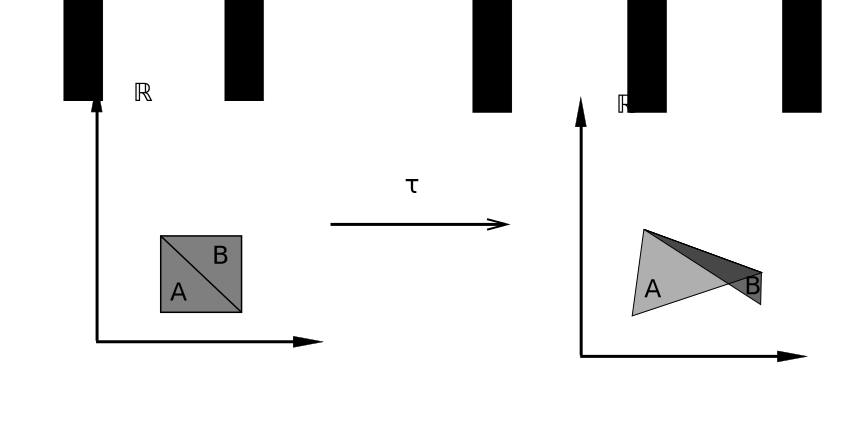
\includegraphics[width=0.9\textwidth]{pictures/Case2}
		\subcaption{}
		\label{Case2}
	\end{subfigure}
	\caption{Darstellung der Dichteverteilung abh\"angig von $\tau$. (a) Die roten Punkte deuten die Dichte in den beiden Scatterplots an, die zwei Vierecke sind Teilmengen des Urbilds, die durch $\tau$ verformt werden. Zu erkennen ist, dass die Streckung des Vierecks zur Erh\"ohung der Entfernung zwischen den Punkten f\"uhrt, was einer Verringerung der Dichte im Viereck entspricht. (b) Der Continuous Scatterplot zweier Dreiecke. Der Grauwert gibt die Dichte an Punkten innerhalb der Dreiecke an.}
	\label{ContinuousScatterplot}
\end{figure}
Das Continuous Scatterplotting stellt eine Erweiterung des Scatterplotting dar, sodass als Urbild statt einer endlichen Anzahl von Objekten auch kontinuierliche Mengen dienen k\"onnen. Die von Bachthaler und Weiskopf\cite{bachthaler2008continuous} vorgestellte Definition wurde von Fritzsch\cite{fritzsch2016continuousScatterplot} um einige wichtige Punkte erweitert. Beim Continuous Scatterplotting wird ein Ansatz verwendet, der dem Verfahren bei der Herleitung der Kontinuumsmechanik aus Systemen mit diskreten Massepunkten \"ahnelt \cite[S.~1429]{bachthaler2008continuous}. Das Ziel des Continuous Scatterplotting ist es, eine Dichtefunktion $\sigma: \mathbb{R}^m \rightarrow \mathbb{R}$ zu finden, die den Punkten des Bildraums, abh\"angig von $\tau$, Dichtewerte zuordnet. $\sigma$ kann als Funktion aufgefasst werden, die jedem Pixel des Scatterplots einen skalaren Wert zuordnet, der z.B. als Farbe oder Opazit\"at dargestellt werden kann. In \cref{ContinuousScatterplot} ist der Effekt, den $\tau$ auf die Dichtefunktion hat, dargestellt. Um $\sigma$ berechnen zu k\"onnen, werden zwei Annahmen getroffen:

Die erste Annahme ist, dass eine Dichtefunktion $s: \mathbb{R}^n \rightarrow \mathbb{R}$ existiert, die jedem Punkt des Urbilds von $\tau$ einen skalaren Wert, die Dichte an diesem Punkt, zuordnet. Der Einfachheit halber wird im Folgenden eine uniforme Dichte von $s(x) = 1$ angenommen. Aus der Dichte an den Punkten l\"asst sich die Gesamtdichte $M$, auch bezeichnet als Masse, einer Teilmenge $V\subset\mathbb{R}^n$ berechnen:

\begin{equation}
M = \int_{V}s(x)d^nx
\label{Dichtefunktion}
\end{equation}

Die zweite Annahme besagt, dass die Masse einer Teilmenge $\phi\subset\mathbb{R}^m$ gleich der Masse ihres Urbildes ist, also $\tau$ die Gesamtdichte nicht beeinflusst. Da $\tau$ in der Regel nicht invertierbar ist, wird $\tau^{-1}(\phi)$ verwendet, um das Urbild von $\phi$ zu notieren. 


F\"ur $\xi \in \Phi$ f\"uhren die Annahmen zu der Gleichung

\begin{equation}
\int_{\phi}\sigma(\xi)d^m\xi = \int_{\tau^{-1}(\phi) = V}s(x)d^nx.
\end{equation}

Da $\tau$ weder injektiv noch surjektiv ist, gilt der umgekehrte Fall nur, wenn zus\"atzlich $\forall x \in V: f^{-1}(f(x)) \subset V$ gilt\cite [S.~20]{fritzsch2016continuousScatterplot}:

\begin{equation}
\int_{V}s(x)d^nx = \int_{\phi = \tau(V)}\sigma(\xi)d^m\xi
\end{equation}

Fritzsch \cite[S.~20~f.]{fritzsch2016continuousScatterplot} definiert zus\"atzlich ein $\sigma_v$, das die Dichtefunktion der Einschr\"ankung von $\tau$ auf $V$ beschreibt, also den \glq Beitrag\grq{} von $V$ zu $\sigma$:

\begin{equation}
\int_{\phi} \sigma_v(\xi)d^m\xi = \int_{\tau|_V^{-1}(\phi)}s(x)d^nx
\end{equation}

Mithilfe der $\sigma_v$ stellt Fritzsch fest, dass f\"ur eine Zerlegung des Definitionsbereichs $U$ von $\tau$ in eine Menge von disjunkten Teilmengen $\hat{V} = {V_i | V_i \in U}$ gilt, dass

\begin{equation}
\begin{split}
\int_{\phi}\sigma(\xi)d^m\xi 
&= \int_{\bigcup\limits_{V_i}\tau|_{V_i}^{-1}(\phi)} s(x)d^nx
\\
&= \sum_{V_i}\int_{\tau|_{V_i}^{-1}(\phi)} s(x)d^nx
\\
&= \sum_{V_i}\int_{\phi}\sigma_{V_i}(\xi)d^m\xi
\\
&= \int_{\phi}\sum_{V_i}\sigma_{V_i}(\xi)d^m\xi.
\end{split}
\end{equation}

Da die Integranden des ersten und letzten Integrals gleich sein m\"ussen, ergibt sich daraus

\begin{equation}
\sigma(\xi) = \sum_{V_i}\sigma_{V_i}(\xi).
\label{DensitySum}
\end{equation}

Eine intuitive Interpretation von \cref{DensitySum} ist, dass die gesamte Dichtefunktion von $\tau$ als Summe der Dichtefunktionen der Einschr\"ankungen von $\tau$ auf die $V_i$ gebildet werden kann.

Die Berechnung von $\sigma$ h\"angt vom Verh\"altnis von $m$ und $n$ zueinander ab. Da in der vorliegenden Arbeit nur der Fall $m=n=3$ auftritt, beschr\"ankt sich die weitere Erl\"auterung auf diesen Fall. F\"ur $m=n$ unterscheiden Bachthaler und Weiskopf folgende F\"alle f\"ur $V \subseteq \mathbb{R}^n$\cite[S.~1430]{bachthaler2008continuous}:

\paragraph{Fall 1: $\tau$ ist differenzierbar und ein Diffeomorphismus}\hspace{200pt}\\
Ein Diffeomorphismus ist eine bijektive, stetig differenzierbare Abbildung, deren Umkehrabbildung ebenfalls stetig differenzierbar ist. 
Wenn $\tau$ ein Diffeomorphismus ist, l\"asst sich durch die Anwendung des Transformationssatzes von Integralen die Gleichung 

\begin{equation}
\int_{\tau(V)}\sigma(\xi)d^{m=n}\xi = \int_{V}\sigma(\tau(x))|det(J_\tau)(x)|d^nx = \int_{V}s(x)d^nx
\end{equation}

bilden, wobei $J_\tau$ die Jacobimatrix von $\tau$ ist. Da der Wert der Determinante der Jacobimatrix von der Position abh\"angig ist, wird der jeweilige Punkt $x$ eingesetzt. Durch weitere Umformungen entsteht die Gleichung

\begin{equation}
\sigma(\xi) = \frac{s(\tau^{-1}(\xi))}{|\det(J_\tau)(\tau^-1(\xi))|}.
\label{Case1Formula}
\end{equation}

Wie schon in Kapitel \hyperref[sec:Grundlagen]{3} erw\"ahnt, entspricht der Betrag der Determinanten der Jacobimatrix dem Betrag der Expandierung oder Schrumpfung der Funktion in der N\"ahe des jeweiligen Punktes. Wenn die Funktion expandiert, nimmt die Dichte ab und wenn sie schrumpft, nimmt die Dichte zu.

\paragraph{Fall 2: $\tau$ ist differenzierbar und konstant \"uber V, V ist keine Nullmenge}\hspace{200pt}\\
Wenn $det(J_\tau) = 0$, dann ist $\tau$ kein Diffeomorphismus und $\sigma$ kann nicht so wie in \textbf{Fall 1} definiert werden. Das ist z.B. der Fall, wenn $\tau$ Bereiche mit konstanten Werten enth\"alt und f\"uhrt dazu, dass eine nicht leere Teilmenge von $\mathbb{R}^n$ auf einen einzelnen Punkt $\xi$ abgebildet wird. Eine M\"oglichkeit die unendlich hohe Dichte an $\xi$ darzustellen und dennoch die Gesamtmasse nicht zu ver\"andern ist es, bei $\xi$ ein Dirac-Delta einzuf\"ugen, das mit dem Volumen aller konstanten Bereiche $V_i \in V$, die nach $\xi$ abgebildet werden, skaliert wird:

\begin{equation}
\begin{split}
\sigma(\xi) &= \sum_{V_i \in V}\delta(\xi - \tau(V_i)) \cdot \int_{V_i}s(x)d^nx\\
&= \sum_{V_i \in V}\delta(\xi - \tau(V_i)) \cdot Vol(V_i).~~~~~~~~~(da~s(x) = 1)
\end{split}
\label{DiracTimesVolume}
\end{equation}

Aus den Eigenschaften des Dirac Deltas und unter der Annahme, dass $s(x) = 1$, ergibt sich, dass die Masseerhaltung erf\"ullt ist:

\begin{equation}
\begin{split}
\int_{\phi}\sigma(\xi)d^n\xi &= \sum_{V_i}\int_{\phi}\delta(\xi - \tau(V_i)) \cdot Vol(V_i)d^n\xi\\
&= \sum_{\forall V_i~:~\tau(V_i)\in \phi} Vol(V_i)\\
&= \int_{\tau^-1(\phi)}1~d^nx
\end{split}
\end{equation}

In \cref{Case2} ist ein Beispielfall daf\"ur angegeben. Die Dichte im \"uberlappenden Bereich der beiden Dreiecke ist gleich der Summe der Dichten der einzelnen Dreiecke. Bei anderen Dichtefunktionen muss \cref{DiracTimesVolume} entsprechend angepasst werden.

\paragraph{Fall 3: $\tau$ ist differenzierbar und kein Diffeomorphismus, V ist Nullmenge}\hspace{200pt}\\
Ein weiterer Fall, in dem $det(J_\tau) = 0$ ist, tritt auf, wenn $V$ eine Nullmenge ist (also z.B. eine Linie im $\mathbb{R}^3$). Da Integration \"uber Nullmengen immer 0 ergibt, k\"onnen die Nullmengen und ihr Bild bez\"uglich $\tau$ einfach aus dem Scatterplotting entfernt werden, ohne die Masseerhaltung zu verletzen.

\paragraph{Fall 4: $\tau$ ist nicht differenzierbar}\hspace{200pt}\\
Wenn im Datensatz Unstetigkeiten auftreten, z.B. zwischen Zellen, ist $\tau$ an diesen nicht differenzierbar. Da die unstetigen Bereiche ebenfalls Nullmengen bilden, kann die gleiche L\"osung wie in \textbf{Fall 3} gew\"ahlt werden.

\begin{figure}
	\begin{subfigure}{0.66\textwidth}
		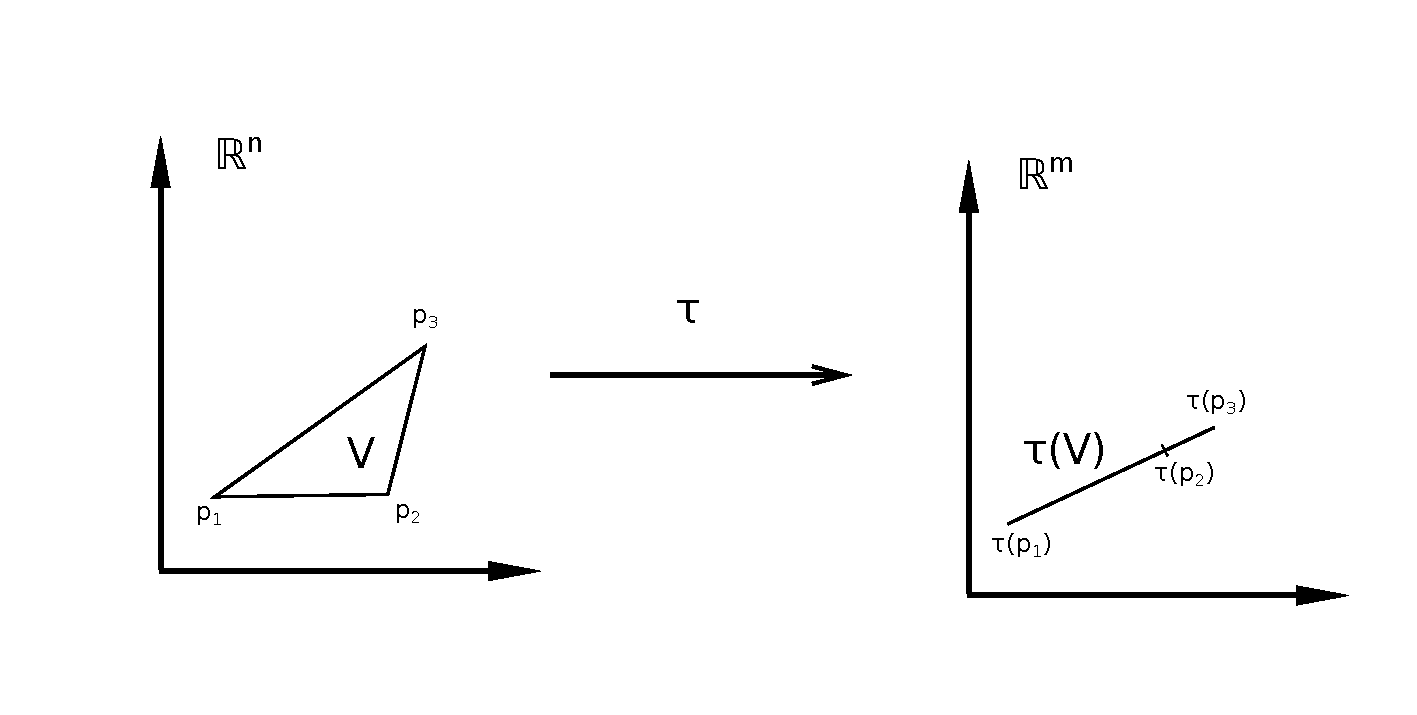
\includegraphics[width=\textwidth]{pictures/Case5}
		\subcaption{}
		\label{Case5}
	\end{subfigure}
	\begin{subfigure}{0.33\textwidth}
		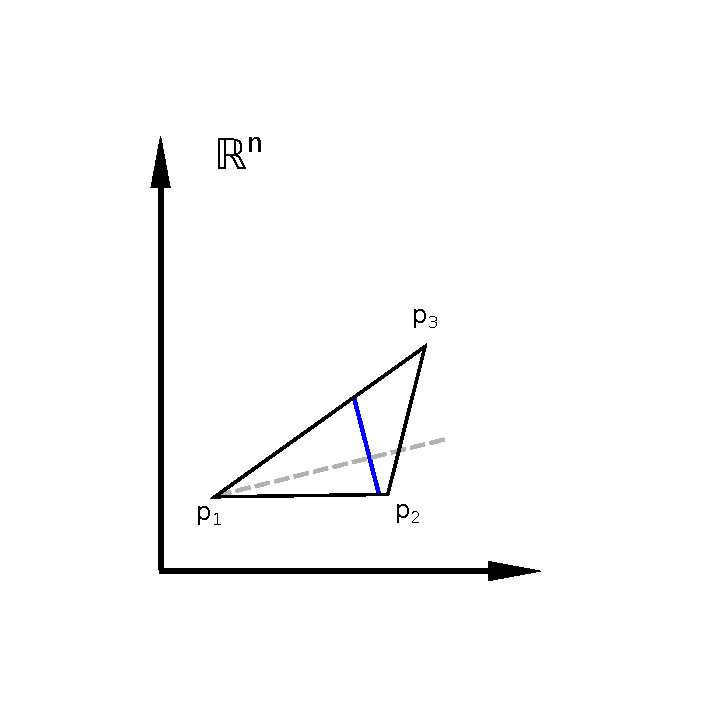
\includegraphics[width=\textwidth]{pictures/Case5-Solution}
		\subcaption{}
		\label{Case5Solution}
	\end{subfigure}
	\caption{Darstellung von \textbf{Fall 5}. (a) Alle drei Punkte des Dreiecks $V$ im linken Koordinatensystem werden auf eine Gerade abgebildet. Dadurch ist $\tau(V)$ eine Nullmenge. (b) Eine Darstellung des von Fritzsch vorgeschlagenen Ansatzes. Die graue, gestrichelte Linie entspricht dem Gradienten, die L\"ange der blauen Linie ist proportional zur Dichte. }
\end{figure}

\paragraph{Fall 5: $\tau$ ist differenzierbar und kein Diffeomorphismus, V ist keine Nullmenge}\hspace{200pt}\\
Von Bachthaler und Weiskopf wurde noch ein f\"unfter Fall genannt, den sie jedoch als nicht in der Praxis vorkommend ansahen. Fritzsch konnte jedoch Beispiele f\"ur diesen Fall angeben\cite[S.~23~f.]{fritzsch2016continuousScatterplot}, die in der Praxis eine Rolle spielen. Ein solcher Fall tritt ein, wenn $V$ keine Nullmenge ist, jedoch auf eine Nullmenge $\tau(V)$ abgebildet wird (siehe \cref{Case5}), wenn also entweder mindestens eine Komponente des Bildes konstant ist, oder eine funktionale Abh\"angigkeit zwischen mindestens zwei Komponenten existiert. 

Die Jacobimatrix enth\"alt in diesem Fall mindestens eine Nullzeile, wodurch gilt, dass $rang(M$ zwischen 0 und $m$ liegt.. 

Fritzsch schl\"agt zur L\"osung dieses Problems zwei Ans\"atze vor. Der Erste orientiert sich an \textbf{Fall 2} und ordnet dem Bildbereich sehr hohe Dichten zu, um die Masseerhaltung zu gew\"ahrleisten. 

Der zweite Ansatz ist nur f\"ur den Fall $m=n=2$ beschrieben, somit muss $rang(M) = 1$ sein. Er kann jedoch auch auf h\"ohere Dimensionen \"ubertragen werden. Ziel ist es, die Dichte an Punkten $p\in\tau(V)$ proportional zur Gesamtmasse der darauf abgebildeten Punkte festzulegen. Dadurch wird zwar die Masseerhaltung nicht erf\"ullt, aber eine interpretierbare Darstellung erzeugt. Dazu werden zun\"acht die Gradienten f\"ur jede Komponente des Bildes von $V$ berechnet. Die Gr\"o{\ss}e der $dim(V) - dim(\tau(V))$-dimensionalen Teilmengen von $V$, die orthogonal zu den durch die Gradienten aufgespannten R\"aumen sind, ist gleich der Masse, die auf die einzelnen Punkte abgebildet wird. Ein Beispiel f\"ur den Fall $dim(V) = 2,~dim(\tau(V)) = 1$ ist in \cref{Case5Solution} zu sehen. Die Dichte an den Punkten von $\tau(V)$ wird dann proportional zur Masse gew\"ahlt.

\subsection{Volumetrische Daten}
Felder, die Punkten im dreidimensionalen Raum bestimmte Werte zuordnen, sind ein h\"aufig vorkommender Typ von Datens\"atzen, der oft unter dem Begriff \glq volumetrische Datens\"atze\grq{} zusammengefasst wird. Dieser Abschnitt beschreibt einen der verbreitetsten Ans\"atze um solche Felder abzuspeichern.  

Ein h\"aufiger Typ von volumetrischen Datens\"atzen beschreibt die Positionen, Formen und Eigenschaften von Objekten im dreidimensionalen Raum. Dazu werden Punkten im $\mathbb{R}^3$ Werte aus einer Menge $\mathbb{M}$ zugeordnet, die den Eigenschaften der Objekten entsprechen. Oft werden bestimmte Werte aus $\mathbb{M}$ daf\"ur verwendet, Punkte zu markieren, an denen sich kein Objekt befindet. Im Fall von $\mathbb{M} = \mathbb{R}^n$ f\"ur ein beliebiges, festes $n$ ist ein solcher Wert, der Punkte au{\ss}erhalb von Objekten markiert, meist das Nullelement. Umgekehrt bedeuten andere Werte, dass sich der Punkt innerhalb eines Objektes befindet.

Das Ergebnis eines Continuos Scatterplotting der Form $m=n=3$ stellt beispielsweise einen volumetrischen Datensatz dar, in dem Punkten ein Dichtewert gr\"o{\ss}er 0 zugeordnet wird, falls sie sich innerhalb eines Objektes befinden. Ansonsten ist die Dichte 0. Da die Visualisierung genau dieser Art von Datens\"atzen die zentrale Aufgabe der vorliegenden Arbeit ist, ist die Abspeicherung und das Auslesen von volumetrischen Daten ein wichtiges Teilproblem.

Bei sehr einfachen Feldern kann es ausreichen, eine Repr\"asentation einer mathematischen Funktion, durch die das Feld approximiert wird, zu speichern. Bei komplexeren Feldern ist dies meistens nicht m\"oglich, da entweder keine hinreichend gut passende Funktion bekannt ist, oder aber die Auswertung der Funktion an einem Punkt sehr viel Rechenzeit ben\"otigen w\"urde, wie z.B. bei aufw\"andigen Simulationen. 

Eine beliebte M\"oglichkeit zur Modellierung von volumetrischen Datens\"atzen besteht darin, den Raum, in dem sich das Objekt befindet, in Volumenelemente, genannt \glq Voxel\grq{}, zu zerlegen, denen Werte zugeordnet werden. Welchem Teil des Voxels, z.B. Mittelpunkt, Eckpunkte, oder Seitenfl\"achen, die Werte zugewiesen werden, ist vom Anwendungsfall abh\"angig. Im einfachsten Fall geben diese Werte bin\"ar an, ob das Voxel ein Objekt schneidet oder nicht. Komplexere Beispiele sind Eigenschaften von Objektst\"ucken oder Teilen des Raums innerhalb des Voxels. Beispiele f\"ur solche Werte sind die Farbe und Opazit\"at eines durchsichtigen Objektes, die Dichte einer Gesteinsschicht oder die von einem Volumen abgegebene Energie bei einer Magnetresonanztomographie. Im Allgemeinen bilden Voxel ein dreidimensionales \"Aquivalent zu Pixeln.

Voxel haben einen entscheidenden Vorteil gegen\"uber anderen volumetrischen Datens\"atzen. Die Komplexit\"at der Daten, und daraus folgend die Rechenzeit der meisten Algorithmen, die Voxel als Eingabe verwenden, ist nicht abh\"angig von der Anzahl und Komplexit\"at der in der urspr\"unglichen Szene dargestellten Objekte, sondern  nur noch von der Anzahl der Voxel, auf die die Szene abgebildet wird. Durch Anpassung der Anzahl der Voxel ist es m\"oglich, Rechenzeit und Qualit\"at der Ergebnisse von Algorithmen gegeneinander abzuw\"agen.

In der Praxis werden Voxel in unterschiedlichen Formen verwendet. Die popul\"arste Variante sind Datens\"atze, die ein quaderf\"ormiges Volumen in gleichgro{\ss}e quaderf\"ormige Voxel zerlegen. Aber auch Datens\"atze mit tetraedrischen Voxeln oder solche, deren Voxel unterschiedliche Formen annehmen, existieren.

\subsection{Volumenvisualisierung}
Zur Darstellung von Objekten werden in der Computergrafik meist Dreiecke verwendet. 
In der Computergrafik werden dreidimensionale Objekte \"ublicherweise durch Dreiecke dargestellt, durch die die Oberfl\"achen der Objekte approximiert werden. Dieses Vorgehen entfernt jedoch alle Informationen \"uber Strukturen im Inneren der Objekte, wie beispielsweise Bereiche gleicher Materialien oder Dichte. Um volumetrische Datens\"atze, wie beispielsweise die Ergebnisse von Continous Scatterplots der Form $m=n=3$, visualisieren zu k\"onnen ohne Informationen \"uber innere Strukturen zu verlieren werden deshalb besondere Verfahren ben\"otigt. Diese werden allgemein unter dem Begriff \glq Volumenvisualisierung\grq{} zusammengefasst. Genauer definiert bezeichnet Volumenvisualisierung Methoden der Extraktion von bedeutungsvollen Informationen aus volumetrischen Daten durch interaktive Grafiken und Bildgebung \cite[S.~127]{hansen2005visualization}. Nachfolgend werden einige Volumenvisualisierung f\"ur skalare Felder  mit Vor- und Nachteilen vorgestellt. Dabei beschr\"anken sich die Erl\"auterungen auf Datens\"atze, die auf, meist quaderf\"ormigen, Voxeln basieren, deren Volumen ein skalarer Wert zugeordnet wurde. F\"ur die meisten Algorithmen existieren jedoch auch Varianten, die mit anderen Formen volumetrischer Daten umgehen k\"onnen.

Nachteile der Speicherung durch Voxel sind unter anderem der hohe Verbrauch an Speicher, da m\"oglicherweise viele tausende Voxel abgespeichert werden m\"ussen, die aus der diskreten Approximierung entstehenden Artefakte, z.B. Treppeneffekte in Bereichen mit pl\"otzlichen Ver\"anderungen, und der Informationsverlust \"uber die urspr\"ungliche Form der abgebildeten Objekte.

\subsubsection{Isofl\"achen}
\begin{figure}
		\centering
		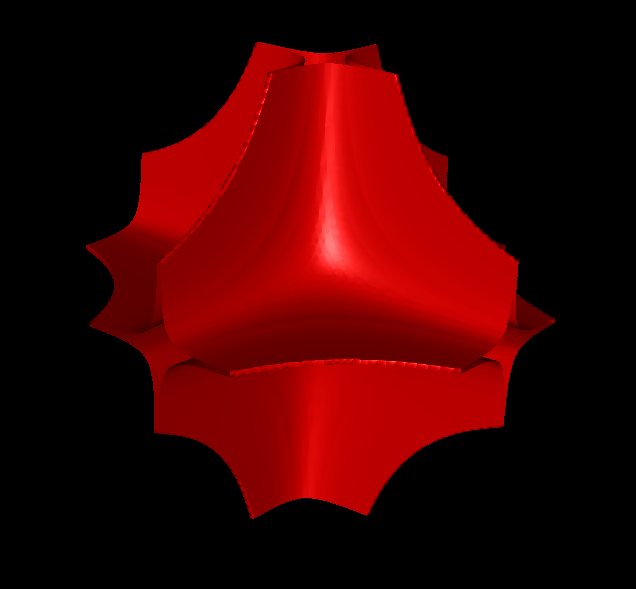
\includegraphics[width=0.35\textwidth]{pictures/isosurface.png}
		\caption{Darstellung einer Isofl\"ache in einem automatisch generierten Datensatz. Erzeugt mithilfe von FAnToM \cite{fantomWebsite}.} 
		\label{Isosurface}
\end{figure}

Volumetrische Datens\"atze beinhalten oft komplexe Strukturen. Die Position und Form sowie die Datenwerte innerhalb dieser Strukturen gut zu vermitteln stellt oft ein zentrales Ziel der Volumenvisualisierung dar. Eine M\"oglichkeit diese Informationen zu vermitteln ist die Berechnung und Darstellung von Isofl\"achen. Die Isofl\"ache einer Funktion $f: \mathbb{R}^3\rightarrow\mathbb{R}$ und eines Isowerts $i \in \mathbb{R}$ ist definiert als eine Oberfl\"ache, die den $\mathbb{R}^3$ in zwei Regionen $R_0, R_1$ teilt, wobei f\"ur jeden Punkt $r_0 \in R_0$ gilt $f(r_0) < i$ und f\"ur jeden Punkt $r_1 \in R_1$ gilt $f(r_1) > i$ \cite[S.~7]{hansen2005visualization}. Die Isofl\"ache muss dabei nicht zusammenh\"angend sein. Auf der Isofl\"ache selbst ist $f$ gleich dem Isowert. 

In \cref{Isosurface} ist ein Beispiel f\"ur eine Isofl\"ache dargestellt. Der Datensatz ist ein Ausschnitt aus der Funktion $f(x,y,z) = cos(x \cdot y \cdot z)$, wobei $x$, $y$ und $z$ im Intervall $[-1;1]$ liegen. Die Datenwerte sind den Eckpunkten der Voxel zugeordnet. 

Die Berechnung von Isofl\"achen stellt eine Herausforderung dar, besonders bez\"uglich der Korrektheit des Verlaufs der Isofl\"achen innerhalb eines Voxels und der ben\"otigten Rechenzeit. In der Vergangenheit wurden viele Verfahren entwickelt, die sich in Hinblick auf Korrektheit und Geschwindigkeit stark unterscheiden. Der wohl einflussreichste davon ist \glq Marching Cubes\grq{} \cite{lorensen1987marching}. Marching Cubes kategorisiert Voxel abh\"angig davon, welche der Werte ihrer Eckpunkte gr\"o{\ss}er oder kleiner als der Isowert sind. F\"ur jede so gebildete Kategorie von Voxeln existiert eine vordefinierte Menge von Dreiecken, die den Verlauf der Isolinie innerhalb dieser Voxel ann\"ahernd beschreiben. F\"ur jedes Voxel werden die Dreiecke der jeweiligen Kategorie korrekt rotiert und zur Isofl\"ache hinzugef\"ugt.

Viele neuere Algorithmen bauen direkt auf Marching Cubes auf, indem sie entweder Fehler des urspr\"unglichen Algorithmus beheben, Optimierungen anbieten oder auf Voxeln anderer Formen (z.B. Tetraeder) anwendbar sind.

Die Visualisierung von volumetrischen Daten mithilfe von Isofl\"achen bietet eine Reihe von Vorteilen. Als Erstes muss die Isofl\"ache nicht neu berechnet werden, solang sich der Isowert nicht \"andert. Die erzeugten Dreiecke k\"onnen mithilfe von 3D Bibliotheken und Grafikkarten sehr schnell und in sehr gro{\ss}er Anzahl dargestellt werden. Auch Rotation, Zoomen und andere Interaktionen brauchen nur vergleichsweise wenig Rechenaufwand. Des Weiteren bieten Isofl\"achen eine ausgezeichnete Darstellung der Form und Position von Strukturen innerhalb eines Datensatzes. Durch Schattierung und Beleuchtung der Dreiecke f\"allt es leicht, dem Benutzer eine Vorstellung der dreidimensionalen Form zu vermitteln.

Indem es dem Benutzer zus\"atzlich erlaubt wird, den Isowert interaktiv festzulegen, z.B. mithilfe eines Textfeldes oder eines Schiebereglers, wird es m\"oglich, Entwicklungen der Werte \"uber den Datensatz hinweg zu analysieren.

Isofl\"achen haben jedoch auch Nachteile. So kann es passieren, dass eine Isofl\"ache, die einen geschlossenen dreidimensionalen K\"orper bildet, den Blick auf Strukturen im Inneren des K\"orpers blockiert. Und zuletzt stellen Isofl\"achen immer nur einen kleinen Teil des Datensatzes gleichzeitig dar, was es erschwert, einen \"Uberblick des gesamten Volumens zu erhalten.

\subsubsection{Slicing}

\begin{figure}
		\centering
		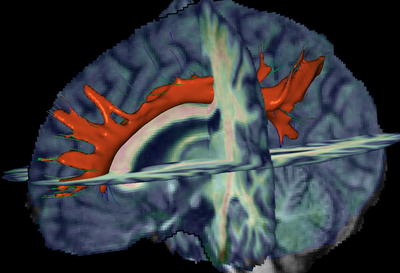
\includegraphics[width=0.4\textwidth]{pictures/slicing.png}
		\caption{Darstellung von drei Slicings durch einen volumetrischen MRI Datensatz. In Orange ist zus\"atzlich eine Isofl\"ache eingezeichnet. Entnommen aus \cite{vis15}.}
		\label{Slicing}
\end{figure}


\label{sec:Slicing}
Ein einfacher Ansatz, um einen volumetrischen Datensatz zu visualisieren ist das sogenannte \glq Slicing\grq{}\cite{munzner2014visualization}. Dabei wird der Schnitt zwischen dem Datensatz und einer Ebene berechnet, und dieser Schnitt durch eine Menge von verbundenen, texturierten Dreiecken, einem sogenannten \glq Dreieckszug\grq{} dargestellt. Form und Position des Dreieckzuges entsprechen dabei der Schnittebene. Mithilfe von Interpolation werden die Werte des volumetrischen Datensatzes an Punkten auf der Oberfl\"ache der Dreiecke berechnet. Das Bestimmen von Werten an Punkten innerhalb der 3D Textur wird als \glq Abtastung\grq{}, die Punkte als \glq Abtastpunkte\grq{} bezeichnet. Um aus den Abtastpunkten die F\"arbungen der Dreiecke zu berechnen, gibt es zwei Verfahren, bezeichnet als Pr\"aklassifizierung und Postklassifizierung.

Bei der Pr\"aklassifizierung wird zun\"achst die Farbe  an den Abtastpunkten bestimmt. Dazu wird eine sogenannte \glq Transferfunktion\grq{} $T$, verwendet die einem Punkt anhand seiner Datenwerte eine Farbe zuordnet. Ein Beispiel f\"ur eine Transferfunktion ist in \cref{Colormap} dargestellt. Die horizontale Achse entspricht den skalaren Werten zwischen Minimum und Maximum im Datensatz sowie den zugeordneten Farben. Die vertikale Achse entspricht der Opazit\"at, von vollst\"andig transparent am unteren Rand bis zu opak am oberen Rand. Durch Position und Farbe der Dreiecke am oberen Rand der Transferfunktion kann die Farbzuordnung festgelegt werden. Die Quadrate stellen interaktiv ausgew\"ahlte Punkte dar, die Zuordnungen von Werten im Skalarfeld zu Farb- und Opazit\"atswerten entsprechen, zwischen denen entlang der verbindenden Linien interpoliert wird. So wird allen Werten im Feld eine Farbe und eine Opazit\"at zugeordnet. Dabei ist zu beachten, dass Opazit\"at im allgemeinen Fall bei Slicing nicht verwendet wird. Um die Farben an allen anderen Punkten der Schnittfl\"ache zu bestimmen, werden die Farben der Abtastpunkte interpoliert. Ein Nachteil der Pr\"aklassifizierung liegt darin, dass durch die Interpolation Farben entstehen k\"onnen, die nicht im Bild der Transferfunktion enthalten sind. Ein Beispiel: Sei $f$ eine Funktion, die Punkten $p \in \mathbb{R}^3$ einen skalaren Wert $s \in \mathbb{R}$ zuordnet, also $f(p) = s$. Sei au{\ss}erdem $V$ ein volumetrischer Datensatz, der einen Ausschnitt von $f$ enth\"alt und $T$ eine Transferfunktion, die Punkte dieses Datensatzes auf eine Farbe aus dem RGBA Farbraum abbildet, die durch einen Tupel $(r,g,b,a)$ dargestellt wird. Die Komponenten des Tupels $(r,g,b,a)$ seien zur Einfachheit auf den Bereich $[0;1]$ skaliert. Zus\"atzlich sei $T(f(p)) = (r,g,b,a)$ definiert als 

\begin{equation}
	f(x)= 
	\begin{cases}
		\text{(1,0; 0,0; 0,0; 1,0) (Rot), wenn } x\leq 0,3\\
		\text{(0,0; 1,0; 0,0; 1,0) (Gr\"un), wenn } 0,3 < x\leq 0,6\\
		\text{(0,0; 0,0; 1,0; 1,0) (Blau), wenn 0,6 < x}.
	\end{cases}
\end{equation}

Seien nun drei Punkte $p_0, p_1$ und $p_2$ definiert, wobei $p_0$ und $p_2$ Abtastpunkte sind, $p_1$ mittig zwischen $p_0$ und $p_2$ liegt sowie $f(p_0) =0,0$ und $f(p_2)=1,0$ gilt. Dann werden bei der Pr\"aklassifizierung zun\"achst die Farben an $p_0$ und an $p_2$ bestimmt und danach die Farbe an $p_1$ durch Interpolation der Farben an $p_0$ und $p_2$ berechnet.
In diesem Beispiel w\"urde $p_0$ das Tupel $(1,0; 0,0; 0,0; 1,0)$, und $p_2$ das Tupel $(0,0; 0,0; 1,0; 1,0)$ zugeordnet werden. Bei linearer, komponentenweiser Interpolation entsteht als Farbe von $p_1$ das Tupel $(0,5; 0,0; 0,5; 1,0)$, ein dunkles Violett. Diese Farbe ist im Bild der Transferfunktion nicht vorhanden. Der Benutzer kann daher den Wert von $f(p_1)$ nicht direkt ablesen, sondern muss zuerst bestimmen, welche Farben gemischt wurden und zu welchen Anteilen. Besonders problematisch ist dies, wenn die Mischfarbe in der Transferfunktion f\"ur einen komplett anderen Wert verwendet wurde, was zu falschen Schl\"ussen \"uber die Verteilung der Werte im Datensatz f\"uhren kann.

Die Postklassifizierung l\"ost diese Probleme, indem die Reihenfolge der Interpolation und Anwendung der Transferfunktion vertauscht wird. Somit werden zun\"achst die Datenwerte interpoliert und danach die Transferfunktion auf die interpolierten Werte angewendet. Dadurch werden Farbverl\"aufe so wie in der Tansferfunktion dargestellt. Es entsteht jedoch der Nachteil, dass durch die Interpolation neue Datenwerte entstehen k\"onnen, die so im Datensatz nicht vorkommen. In den meisten F\"allen wird dies jedoch als das geringere \"Ubel angesehen, weshalb Postklassifizierung fast immer bevorzugt wird. In \cref{Slicing} sind drei Slicings zusammen mit einer orangenen Isofl\"ache abgebildet.

Indem Interaktionen angeboten werden, durch die der Benutzer Position und Orientierung der Schnittfl\"ache interaktiv anpassen kann, bietet Slicing eine gute M\"oglichkeit um die Verteilung von Werten innerhalb eines volumetrischen Datensatzes zu analysieren und Werte ablesen zu k\"onnen. Der Rechenaufwand ist geringer als bei der Berechnung der Isofl\"achen und macht es m\"oglich, die Slicings ohne sp\"urbare Verz\"ogerung zu repositionieren. Slicings eignen sich auch, um andere Volumenvisualisierung zu erg\"anzen, wie z.B. die Isofl\"ache in \cref{Slicing}.

Die gro{\ss}en Nachteile von Slicings liegen in der Schwierigkeit, korrekte Positionen und Orientierungen zu finden, um interessante Bereiche sichtbar zu machen sowie darin, dass die Form von dreidimensionalen Strukturen relativ schlecht vermittelt wird. 

\subsubsection{Direct Volume Rendering}
\label{sec:DVR}
\begin{figure}
	\begin{minipage}{0.45\textwidth}
		\centering
		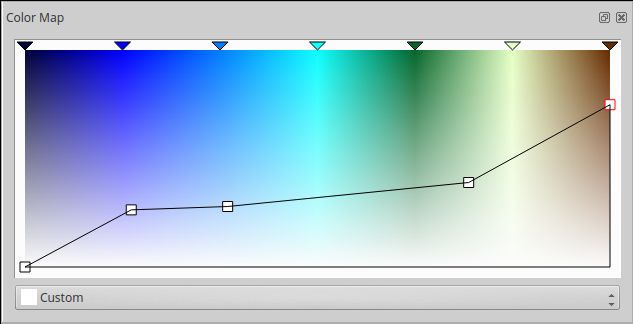
\includegraphics[width=0.9\textwidth]{pictures/Colormap.png}
		\caption{Eine Implementierung einer interaktiven Transferfunktion in FAnToM.} 
		\label{Colormap}
	\end{minipage}
	\hspace{0.08\textwidth}
	\begin{minipage}{0.45\textwidth}
		\centering
		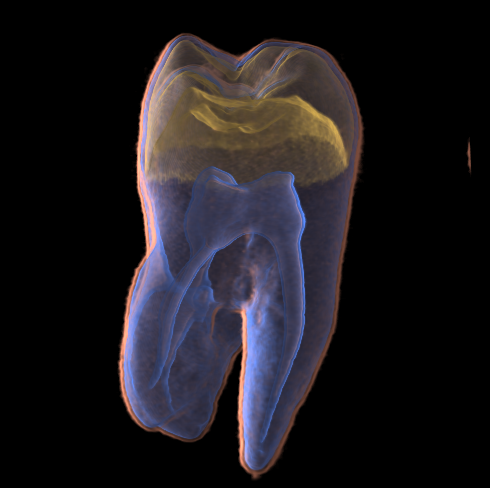
\includegraphics[width=0.47\textwidth]{pictures/Zahn.png}
		\caption{Ein Direct Volume Rendering eines Zahns. Entnommen aus \cite[S.~6]{drebin1988volume}}
		\label{Zahn}
	\end{minipage}
\end{figure}

Die bisher vorgestellten Volumenvisualisierung Verfahren stellten immer nur einen kleinen Teil des volumetrischen Datensatzes gleichzeitig dar. Das hat den Vorteil, dass ein Benutzer nur einen Teil der Daten gleichzeitig interpretieren muss, bringt jedoch eine Reihe von Nachteilen mit sich. Erstens wird vorausgesetzt, dass der Benutzer durch Interaktion unterschiedliche Bereiche ausw\"ahlt, um sich einen \"Uberblick \"uber den Datensatz zu verschaffen, was abh\"angig von Gr\"o{\ss}e und Komplexit\"at viel Zeit und Aufmerksamkeit des Nutzers in Anspruch nehmen kann. Zweitens besteht dabei das Risiko, dass Merkmale des Datensatzes, die nur bei sehr bestimmten Einstellungen sichtbar sind, \"ubersehen werden. Und drittens muss der Benutzer zus\"atzliche mentale Arbeit verrichten, um die jeweils angezeigten Teile in seiner Vorstellung zusammenzusetzten, damit er ein vollst\"andiges Verst\"andnis des Datensatzes entwickeln kann. Dies kann, wiederum abh\"angig von Gr\"o{\ss}e und Komplexit\"at, bei manchen Datens\"atzen fast unm\"oglich sein.

Der Begriff \glq Direct Volume Rendering\grq{} (DVR) bezeichnet eine Reihe von Verfahren der Volumenvisualisierung, die den gesamten Datensatz gleichzeitig darstellen k\"onnen. Daher stammt auch das \glq Direct\grq{} im Namen dieser Gruppe von Verfahren: Anstelle den Datensatz durch einen Querschnitt (Slicing) oder durch eine Oberfl\"ache darzustellen, wird versucht, den gesamten Datensatz direkt zu visualisieren. Ein gro{\ss}er Teil der Informationen in diesem Abschnitt stammt aus dem Buch \glqq The Visualization Handbook\grqq{} \cite{hansen2005visualization}.

\"Ahnlich wie beim Slicing wird eine Transferfunktion verwendet, um den Voxeln eine Farbe zuzuordnen. Zus\"atzlich legt die Transferfunktion auch noch einen Wert im Intervall $[0;1]$ als Opazit\"at fest, die ausdr\"uckt, wie stark ein Voxel hinter ihm gerenderte Voxel \"uberdeckt, wie schon in \cref{sec:Slicing} beschrieben. Eine Opazit\"at von 1 bedeutet dabei, dass das Voxel komplett opak ist, eine Opazit\"at von 0 dagegen dass das Voxel vollst\"andig durchsichtig und damit in der Visualisierung unsichtbar ist. Ein Beispiel f\"ur ein durch Direct Volume Rendering erzeugtes Bild zeigt \cref{Zahn}. 

\begin{figure}
	\centering
	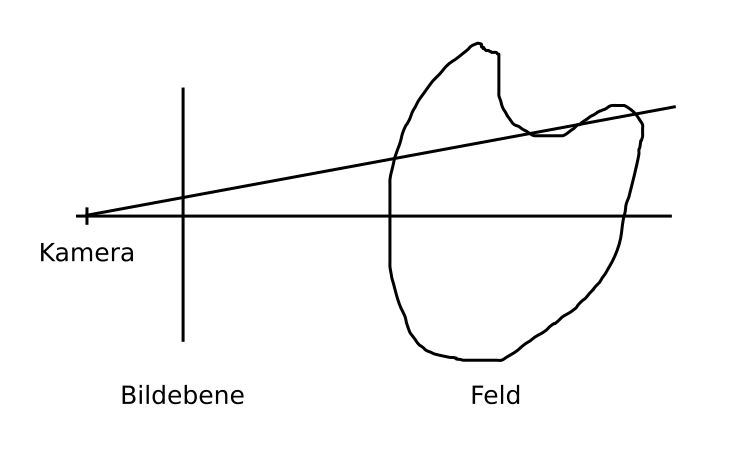
\includegraphics[width=0.5\textwidth]{pictures/DVR}
	\caption{Schematische Darstellung der \textit{image-order} Verfahren. Farbwerte an Positionen auf der Bildebene werden mittels Abtastung entlang von Strahlen, die an der Kameraposition beginnen und die Position auf der Bildebene sowie den Datensatz schneiden, bestimmt.}
	\label{image-order}
\end{figure}

DVR-Verfahren gliedern sich in vier Gruppen, die als \textit{image-order}, \textit{object-order}, \textit{hybride} und \textit{Domain}-Verfahren bezeichnet werden.

Allen \textit{image-order} Verfahren ist gemein, dass sie eine Position im Raum als \glq Kameraposition\grq{} festlegen, die Position, von der aus der Benutzer den Datensatz betrachtet. Diese Position befindet sich dabei im gleichen Koordinatensystem wie die Voxel selbst. Vor der Kamera, orthogonal zur Blickrichtung, wird eine imagin\"are Ebene platziert, die sogenannte Bildebene. Ihre Gr\"o{\ss}e und Position ist so gew\"ahlt, dass sie das gesamte Blickfeld der Kamera einnimmt (siehe \cref{image-order}). Indem Positionen der Bildebene auf Pixel des Bildschirms abgebildet werden, ist es m\"oglich, durch Einf\"arbung der Bildebene eine Visualisierung zu erzeugen. Die Farbe eines Pixels ergibt sich dabei, indem ein Strahl berechnet wird, der sowohl durch die Position des Mittelpunkts des Pixels auf der Bildebene als auch durch die Kameraposition verl\"auft. Entlang des Strahls werden Abtastpunkte gew\"ahlt, an denen die Transferfunktion ausgewertet wird. Genau wie beim Slicing k\"onnen dabei Pr\"a- und Postklassifizierung verwendet werden. Abh\"angig davon, wie die Farb- und Opazit\"atswerte der Abtastpunkte kombiniert werden, k\"onnen unterschiedliche Darstellungen entstehen. Eine Reihe davon wird sp\"ater im Text vorgestellt. Da die Kombination von Farb- und Opazit\"atswerten in OpenGL fast immer durch die Funktion des Blendings implementiert wird, verwenden wir den Begriff \glq Blending\grq{} im Folgenden synonym dazu. Bei manchen Varianten ist es m\"oglich, die Berechnung der Farbe eines Pixels fr\"uhzeitig zu beenden, wenn die berechneten Farb- und Opazit\"atswerte bestimmte Werte annehmen. In diesem Fall wird davon ausgegangen, dass der Einfluss der noch zu berechnenden Abtastpunkte zu klein ist, um vom Benutzer noch wahrgenommen zu werden. Diese fr\"uhzeitige Terminierung ist einer der wichtigsten Vorteile der \textit{image-order} Verfahren. 

Im Gegensatz dazu zerlegen \textit{object-order} Verfahren den volumetrischen Datensatz in eine Menge von Basiselementen oder Basisfunktionen, die auf eine Bildebene projiziert werden und dadurch eine Darstellung des Datensatzes bilden. Wenn sich Projektionen der Basiselemente \"uberlappen, was f\"ur die meisten Datens\"atze praktisch der Standardfall ist, werden die Farbwerte abh\"angig von gew\"ahltem Verfahren mittels Blending kombiniert. Genau wie bei den \textit{image-order} Verfahren k\"onnen unterschiedliche Varianten des Blendings gew\"ahlt werden, was zu unterschiedlichen Visualisierungen f\"uhrt. Der gr\"o{\ss}te Vorteil von \textit{object-order} Verfahren liegt darin, dass nur die Voxel abgespeichert und verarbeitet werden m\"ussen, die einen skalaren Wert ungleich 0 enthalten. Das ist besonders gut, da die Rechenzeit von \textit{object-order} Verfahren in der Regel direkt von der Anzahl zu verarbeitender Voxel abh\"angt. Ein Problem liegt darin, dass es f\"ur viele Verfahren notwendig ist, die Voxel abh\"angig von ihrer Entfernung zur Kamera zu sortieren. Diese Sortierung muss aktualisiert werden, wenn die Kamera bewegt wird.

\textit{Hybride} Verfahren versuchen Vorteile von  \textit{image-order} , wie die fr\"uhzeitige Terminierung, und \textit{object-order} Verfahren, wie den geringen Speicherverbrauch und die Abh\"angigkeit der Rechenzeit von der Anzahl an Voxeln, zu kombinieren. Die Details der Implementierung unterscheiden sich jedoch stark zwischen den einzelnen Verfahren. 

Zuletzt gibt es noch die \textit{Domain}-Verfahren. Dabei wird der komplette Datensatz so transformiert, dass die DVR Visualisierung mittels mathematischer Eigenschaften des Wertebereichs (englisch \glq Domain\grq{}) erzeugt werden kann. Ein Beispiel daf\"ur ist, den Datensatz zun\"achst mittels der Fourier Transformation in den Frequenzraum zu \"uberf\"uhren. Indem im Frequenzraum ein bestimmter zweidimensionaler Ausschnitt gew\"ahlt und zur\"uck in den Ortsraum transformiert wird, kann eine Projektion des urspr\"unglichen Datensatzes erzeugt werden. Ein gro{\ss}er Vorteil von \textit{Domain}-Verfahren liegt h\"aufig in der sehr viel k\"urzeren Rechenzeit.

Bei einer Eingabe von $N\times N\times N$ Voxeln hat die bereits erw\"ahnten Variante im Frequenzraum beispielsweise eine Komplexit\"at von $O(N^2 log(N))$ statt den bei \textit{object-order} Verfahren \"ublichen $O(N^3)$. Leider schr\"ankt dieses Verfahren die m\"oglichen erzeugbaren Visualisierungen auf ein simples Integral entlang der Sichtstrahlen ein $O(N^3)$ \cite[S.~143]{hansen2005visualization}. Es existieren Ergebnisse, die versuchen andere Visualisierungen zu approximieren. Jedoch stellt dies eine deutliche Einschr\"ankung des DVR dar, weshalb im Folgenden \textit{Domain}-Verfahren nicht weiter betrachtet werden.

\begin{figure}
	\centering
	\begin{subfigure}{0.24\textwidth}
		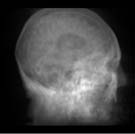
\includegraphics[width=\textwidth]{pictures/Xray.png}
		\subcaption{}
		\label{DVR:Xray}
	\end{subfigure}
	\begin{subfigure}{0.24\textwidth}
		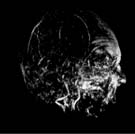
\includegraphics[width=\textwidth]{pictures/MIP.png}
		\subcaption{}
		\label{DVR:MIP}
	\end{subfigure}
	\begin{subfigure}{0.24\textwidth}
		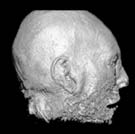
\includegraphics[width=\textwidth]{pictures/Iso.png}
		\subcaption{}
		\label{DVR:Isosurface}
	\end{subfigure}
	\begin{subfigure}{0.24\textwidth}
		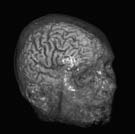
\includegraphics[width=\textwidth]{pictures/Trans.png}
		\subcaption{}
		\label{DVR:Translucent}
	\end{subfigure}
	\caption{Arten von DVR Visualisierungen: (a) R\"ontgenbild, (b) Maximum Intensity Projection, (c) Isofl\"achenartig, (d) Transluzent. Entnommen aus \cite[S.~134]{hansen2005visualization}}
	\label{DVRModes}
\end{figure}
Es existieren vier popul\"are Arten von Visualisierungen, die durch DVR-Verfahren erzeugt werden k\"onnen. In \cref{DVRModes} sind diese Visualisierungen am Beispiel des gleichen Datensatzes, eines menschlichen Kopfes, dargestellt.

\paragraph{R\"ontgenbild}
Die Bezeichnung \glq R\"ontgenbild\grq{} stammt aus der \"Ahnlichkeit der entstehenden Bilder zu denen, die beim klassischen R\"ontgen in der bildgebenden Medizin erzeugt werden. Die F\"arbung eines Pixels ergibt sich in diesem Verfahren dadurch, dass die ermittelten Farb- und Transparenzwerte aller zur F\"arbung des Pixels beitragenden Voxel aufaddiert werden. Damit sind die Voxel gemeint, die z.B. vom selben Strahl durch den Mittelpunkt des Pixels geschnitten werden (\textit{image-order}) oder deren Basisfunktionen sich in diesem Pixel \"uberschneiden (\textit{object-order}). Das Blending entspricht in diesem Fall einer Addition, die die Farbe eines Voxels auf die bisher bestimmte Farbe eines Pixels aufaddiert. Ein Beispiel f\"ur ein so erzeugtes Bild ist in \cref{DVR:Xray} zu sehen. 

\paragraph{Maximum Intensity Projection (MIP)}
Bei der MIP wird zun\"achst das Voxel mit dem h\"ochsten Skalarwert berechnet, der auf diesen Pixel abgebildet wird, z.B. per Strahl oder Projektion der Basisfunktion. Nachdem dieser Wert bestimmt wurde, wird auf ihn die Transferfunktion angewendet und das Ergebnis als Farbe des Pixels festgelegt. Das Blending entspricht einer Maximumsfunktion, die den h\"ochsten bisher f\"ur einen Pixel gefundenen Skalarwert und den Skalarwert des Voxels entgegennimmt und das Maximum der beiden ausgibt. \cref{DVR:MIP} zeigt ein durch MIP erstelltes Bild. 


\paragraph{Isofl\"achenartig}
Wenn die Transferfunktion genau einen Wert $x$ auf eine Opazit\"at von $1,0$ abbildet und alle anderen Werte auf Opazit\"aten von $0,0$, so \"ahneln die erzeugten Bilder Isofl\"achen. Blending entspricht hierbei einer Minimumsfunktion, die anstelle der Farbwerte die Distanz zur Kamera zur Entscheidung verwendet. Abh\"angig vom Verfahren kann auch sofort terminiert werden, wenn ein opakes Voxel gefunden wurde. Dies erschwert jedoch das sp\"atere Hinzuf\"ugen von z.B. Schatten. Durch geschickte Wahl der Reihenfolge, in der die Voxel verarbeitet werden, z.B. mit zunehmender Entfernung zur Kamera, kann weitere Beschleunigung erreicht werden. In \cref{DVR:Isosurface} ist eine so erzeugte isofl\"achenartige Darstellung gezeigt.

\paragraph{Transluzent}
\"Ahlich wie beim R\"ontgenbild k\"onnen auch bei transluzenten Bildern die Transferfunktionen Werte zwischen $0$ und $1$ annehmen. Dabei werden Voxel, deren Opazit\"at weder $0$ noch $1$ ist als teilweise transparent dargestellt. Dazu m\"ussen die Farben und Opazit\"aten von Voxeln, die zur Farbe eines Pixels beitrage, korrekt kombiniert werden, sodass transparente Voxel die Sicht auf dahinterliegende Strukturen freigeben. Die Formulierung des Blendings h\"angt hierbei von der Verarbeitungsreihenfolge der Voxel ab. In Abschnitt \ref{sec:Raycasting} wird dies genauer erl\"autert. Transluzente Visualisierungen sind besonders popul\"ar, da sie sowohl hohe Flexibilit\"at durch Wahl der Transferfunktion aufweisen als auch den Grundgedanken des DVR, das gleichzeitige und vollst\"andige Darstellen des Datensatzes, am besten umsetzen. Der Rest der Arbeit besch\"aftigt sich deshalb ausschlie{\ss}lich mit Verfahren zur Erzeugung von transluzenten Visualisierungen. Ein Beispiel f\"ur ein durch Transluzentes DVR erzeugtes Bild ist in \cref{DVR:Translucent} zu sehen. Transluzente Verfahren stellen eine Verallgemeinerung des Verfahrens zur Erzeugung von Isofl\"achen dar.

\section{Direct Volume Rendering Verfahren}
Es existieren eine Reihe von DVR-Verfahren, die die in \cref{sec:DVR} erl\"auterten Konzepte umsetzen. Diese Verfahren bieten dabei individuelle Vor- und Nachteile, die in Hinblick auf die Anforderungen der Anwendung verglichen werden m\"ussen. In diesem Kapitel werden dazu zun\"achst einige der wichtigsten DVR-Verfahren vorgestellt und am Ende miteinander verglichen, um das f\"ur die Problemstellung geeignetste Verfahren auszuw\"ahlen. 

\subsection{Texture Slicing}
\label{sec:TextureSlicing}
Eines der ersten \textit{image-order} DVR-Verfahren wurde von Neumann und Cullip \cite{cullip1993accelerating} entwickelt. Es wird aufgrund der darin verwendeten Mechanismen meist als Texture Slicing bezeichnet, in manchen Ver\"offentlichungen aber auch als Raycasting. Dieser Begriff wird jedoch auch f\"ur ein anderes Verfahren verwendet, das sp\"ater in dieser Arbeit vorgestellt wird.

\begin{figure}
	\centering
	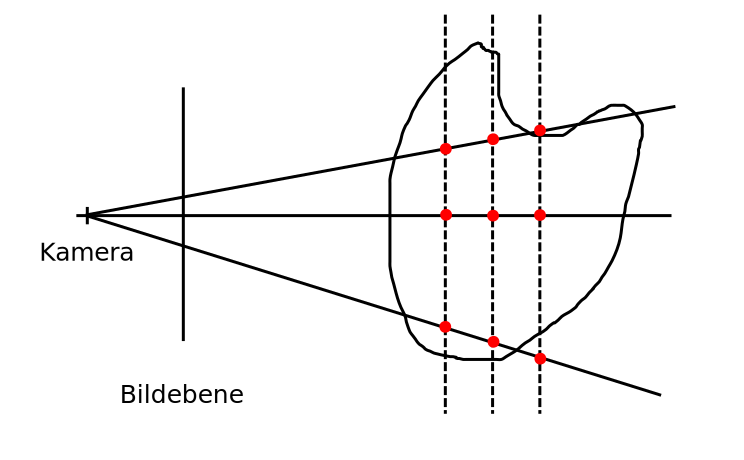
\includegraphics[width=0.6\textwidth]{pictures/Texture_Slicing}
	\caption{Schematische Darstellung des Texture Slicings. Die gestrichelten Linien entsprechen Schnittbildern durch den Datensatz. Die roten Punkte stellen die Positionen auf den Schnittbildern dar, die auf das Pixel des jeweiligen Strahls projiziert werden.}
	\label{TextureSlicing}
\end{figure}

Beim Texture Slicing werden mehrere imagin\"are Ebenen parallel zur Bildebene durch den Datensatz gelegt. Diese Schnittebenen werden nach einem Verfahren eingef\"arbt, das praktisch identisch zu dem in \cref{sec:Slicing} beschriebenen Slicing ist. Die entstandenen Schnittbilder werden danach auf die Bildebene projiziert und durch Blending miteinander kombiniert. Die f\"ur das Blending verwendete Formel h\"angt von der Reihenfolge ab, in der die Schnitte miteinander kombiniert werden. Wenn die Schnitte mit zunehmender Entfernung zur Kamera (front-to-back) verarbeitet werden, entspricht das Blending den Formeln

\begin{align}
&c_n = c_{n-1} + c_{s}\cdot(1-\alpha_{n-1})\cdot\alpha_{s}
\label{front-to-back-color}\\ 
&\alpha_n = \alpha_{n-1} + \alpha_{s}\cdot(1-\alpha_{n-1}).
\label{front-to-back-alpha}
\end{align}

Dabei steht $c_n$ f\"ur die nach dem Blending von $n$ Schnittfl\"achen akkumulierte Farbe, $\alpha_n$ f\"ur die akkumulierte Opazit\"at. Das Blending wird initialisiert mit den Werten $c_0 = \alpha_0 = 0$. Die Parameter $c_{s_n}$ und $\alpha_{s_n}$ entsprechen der Farbe und Opazit\"at der $n$-ten Schnittfl\"ache. Das Blending wird pixelweise durchgef\"uhrt. Wenn sich der Wert von $\alpha_{n-1}$ in Pixeln nah genug an 1 ann\"ahert, k\"onnen diese in sp\"ateren Blending Schritten \"ubersprungen werden, da der Einfluss dieser Blendings auf die Farbe der Pixel sehr klein ist. Dies setzt jedoch voraus, dass das Blending dahingehend konfigurierbar ist, was nicht in allen Versionen von OpenGL oder anderen Renderingsystemen der Fall ist. 

Wenn die Schnitte dagegen mit abnehmender Entfernung zur Kamera verarbeitet werden (back-to-front), ergeben sich f\"ur das Blending die Gleichungen

\begin{align}
&c_n = (1-\alpha_{s_n})\cdot c_{n-1}+c_{n_s}\cdot\alpha_{s_n}
\label{back-to-front-color}\\ 
&\alpha_n = (1-\alpha_{s_n})\cdot\alpha_{n-1} + \alpha_{s_n}.
\label{back-to-front-alpha}
\end{align}

Dabei ist fr\"uhzeitiges Terminieren nicht m\"oglich, weshalb die back-to-front Reihenfolge selten verwendet wird.

Ein Problem des Texture Slicings liegt darin, dass die gew\"ahlte Anzahl der Schnittfl\"achen einen Einfluss auf das erzeugte Bild hat. Wenn innerhalb der gleichen Distanz von der Kameraposition aus mehr Schnittfl\"achen berechnet werden, muss das Blending mehr Summanden aufaddieren. Mehr Schnittfl\"achen f\"uhren also zu h\"oheren aufaddierten Opazit\"aten und damit zu anderen Bildern. Eine oft angewendete L\"osung liegt darin, die von der Transferfunktion bestimmte Opazit\"at mit dem Inversen der Anzahl der Schnittfl\"achen zu skalieren.

Die Laufzeit des Texture Slicings ist haupts\"achlich abh\"angig von der Anzahl der einzuf\"arbenden Pixel und der Nummer der zu berechnenden Schnittbilder. Eine h\"ohere Anzahl von Schnittbildern f\"uhrt jedoch auch zu einer exakteren Repr\"asentation des Datensatzes, da sich dadurch die Chance, dass ein relevanter Teil des Datensatzes von keinem der Schnitte getroffen wird, reduziert. Durch Interaktionen kann es dem Benutzer erm\"oglicht werden, den Tradeoff zwischen Rechenzeit und Bildqualit\"at anzupassen.

Der wichtigste Vorteil des Texture Slicings ist die f\"ur \textit{image-order} Verfahren relativ geringe Rechenzeit. Sowohl das Erstellen der Schnittbilder als auch die Durchf\"uhrung des Blendings k\"onnen effizient von Grafikkarten parallelisiert werden. Ein wichtiger Nachteil ist jedoch, dass die Entfernung der Schnittpunkte von Strahl und Schnittebenen sich von Strahl zu Strahl unterscheiden: Im Zentrum des Sichtfeldes liegen die Schnittpunkte n\"aher zusammen als am Rand. Dies f\"uhrt dazu, dass die Bildqualit\"at zum Rand hin abnimmt (siehe \cref{TextureSlicing}). Zudem werden d\"unne, zur Bildebene parallele Strukturen vom Texture Slicing oft zu schwach oder gar nicht dargestellt, da zu wenige Schnittpunkte mit den Schnittebenen existieren.

\subsection{Raycasting}
\label{sec:Raycasting}

Historisch entwickelte sich das heutige Raycasting aus den Texture Slicing Verfahren. Es versucht, die Probleme des Texture Slicings, die durch die Verwendung der Schnittebenen entstehen, zu Lasten der Laufzeit zu beheben.

Dazu wird die Bestimmung der Farbwerte der Pixel als approximierte Berechnung von Linienintegralen aufgefasst. Der Datensatz wird zun\"achst als Wolke von Partikeln aufgefasst, wobei die Partikel Licht emitieren und absorbieren \cite[s.~134~f.]{hansen2005visualization}. Wie viel Licht Partikel in einem Voxel absorbieren und emittieren sowie die Farbe des emitierten Lichts wird \"uber die Transferfunktion beschrieben. Das aus Richtung der Strahlen zur Kameraposition hin auf der Bildebene eintreffende Licht entspricht dann dem Integral 

\begin{equation}
I(x,r) = \int_{0}^{L} C(s)\mu(s) e^{-\int_{0}^{s}\mu(t)dt}ds.
\end{equation}

Dabei entspricht $x$ der Position auf der Bildebene, $r$ der Richtung des Strahls von der Kameraposition aus durch $x$, $L$ der L\"ange des Strahls, bis er zum letzten Mal einen Voxel schneidet, $C(s)$ dem an Position $s$ emittierten Licht und $\mu(s)$ dem Okklusionskoeffizienten an $s$, also dem Anteil von Licht, das an $s$ absorbiert wird, wobei $\mu(s) \in [0;1]$. Somit emittiert jeder Punkt $p$ eines Strahls Licht und absorbiert gleichzeitig einen Teil des Lichts, das von den anderen Punktes des Strahls, die weiter von der Kamera entfernt sind als $p$, emittiert wird. Der Anteil des Lichts, den $p$ absorbiert, entspricht der Opazit\"at des Voxels, in dem $p$ liegt.

Dieses Integral l\"asst sich im allgemeinen Fall nur mit viel Rechenaufwand, wenn \"uberhaupt, automatisch berechnen \cite[S.~136]{hansen2005visualization}. Um die Rechenzeit zu verringern, kann das Integral approximiert werden. Durch Vereinfachungsschritte, die hier aus Gr\"unden der L\"ange \"ubersprungen werden, ergibt sich die Formel

\begin{equation}
I(x,r) = \sum_{i=0}^{L/\Delta s - 1} C(i\Delta s)\alpha(i\Delta s) \prod_{j=0}^{i-1}( 1 - \alpha(j \Delta s)).
\end{equation}

Hier entspricht $\Delta s$ einem Bruchteil von $L$. Desto kleiner $\Delta s$ wird, desto besser wird das Integral approximiert. Die Funktion $\alpha(i \Delta s)$ ermittelt die Opazit\"at an dem Punkt des Strahls, der $i \Delta s$ von der Kamera entfernt ist. 

Um die schon beim Texture Slicing beschriebenen Probleme 

 zu vermeiden, wird die Opazit\"at direkt mit der Entfernung zwischen den Abtastpunkten auf einem Strahl skaliert, die proportional zum Inversen der Anzahl der Abtastpunkte pro Strahl ist.
Die Gleichung kann \"aquivalent durch zwei rekursive Folgen ausgedr\"uckt werden (f\"ur $i > 0$):

\begin{align}
&\alpha_0 = c_0 = 0\\
&c_i = C(i\Delta s)\cdot\alpha(i\Delta s)\cdot(1-\alpha_{i-1}) + c_{i-1} \label{RaycastingFormula1}\\
&\alpha_i = \alpha\cdot(i \Delta s)\cdot(1-\alpha_{i-1}) + \alpha_{i-1} \label{RaycastingFormula2}
\end{align} 

Diese rekursiven Funktionen entsprechen der Abtastung entlang des Strahls ausgehend von der Kamera (front-to-back). Wenn $\alpha_i$ sich nah genug an 1 ann\"ahert kann die Berechnung fr\"uhzeitig terminieren. F\"ur die umgekehrte Richtung (zur Kamera hin, back-to-front) ergibt sich

\begin{align}
&\alpha_0 = c_0 = 0\\
&c_i = c_{i-1}\cdot(1 - \alpha(i\Delta s)) + C(i\Delta s)\cdot\alpha(i\Delta s)\\
&\alpha_i = \alpha_{i-1}\cdot(1 - \alpha(i\Delta s)) + \alpha(i \Delta s).
\end{align}

Dies hat jedoch den Nachteil, dass fr\"uhzeitiges Terminieren nicht m\"oglich ist, weshalb diese Variante nur sehr selten benutzt wird.

Durch Verwendung der rekursiven Gleichungen wird der Farbwert eines Pixels bestimmt ohne Zwischenergebnisse in eine Textur schreiben zu m\"ussen. Daher wird beim Raycasting kein Blending im Sinne der Funktion von OpenGL ben\"otigt. Die Farb- und Opazit\"atswerte m\"ussen jedoch trotzdem durch Gleichungen kombiniert werden, die \"aquivalent zu denen beim Blending sind.


\begin{figure}
	\centering
	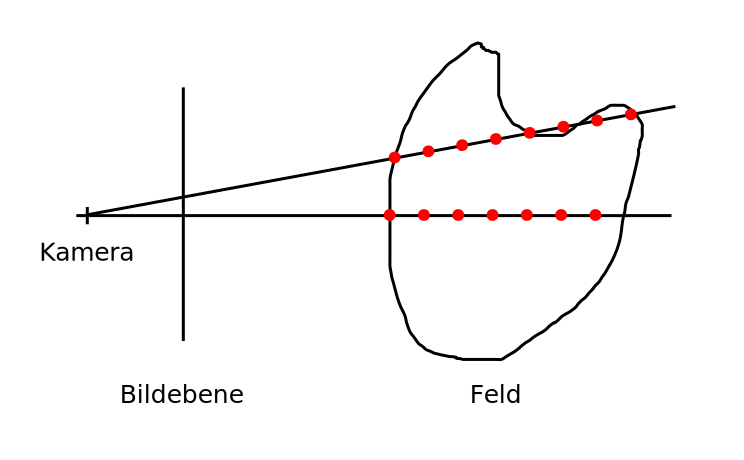
\includegraphics[width=0.6\textwidth]{pictures/Raycasting}
	\caption{Schematische Darstellung des Raycastings. Die roten Punkte stellen Abtastpunkte dar, die in regelm\"a{\ss}igen Abst\"anden auf den Strahlen liegen.}
	\label{Raycasting}
\end{figure}

Eine direkte Umsetzung der front-to-back Funktionen traversiert den Datensatz entlang der Strahlen und berechnet das emittierte und absorbierte Licht an Abtastpunkten, die in regelm\"a{\ss}igen Abst\"anden auf den Strahlen liegen, was der \"ublichen Herangehensweise bei \textit{image-order} Verfahren entspricht. Es ist dabei sinnvoll, Abtastpunkte erst innerhalb des Datensatzes, also im oder am Rand des ersten geschnittenen Voxels zu setzen. In \cref{Raycasting} wird Raycasting mit dieser Optimierung schematisch dargestellt. 
Da f\"ur dieses Verfahren Strahlen durch das Volumen berechnet werden, entlang derer abgetastet wird, bezeichnet man es als Raycasting. Die Vorteile des Raycastings liegen in der schon angesprochenen M\"oglichkeit zur fr\"uhzeitigen Terminierung und der M\"oglichkeit, die Anzahl der Abtastpunkte festzulegen. Die Distanz zwischen Ein- und Austrittspunkt eines Strahls in die 3D Textur geteilt durch die Anzahl an Abtastpunkten auf dem Strahl wird als \glq Abtastrate\grq{} bezeichnet.

\begin{figure}
	\begin{minipage}{0.49\textwidth}
		\centering
		\begin{subfigure}{0.7\textwidth}
			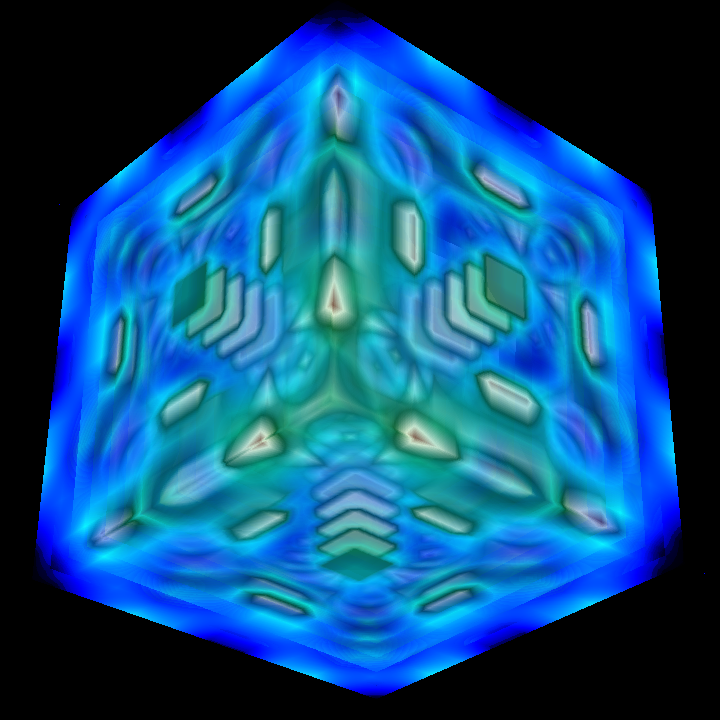
\includegraphics[width=\textwidth]{pictures/DVR1.png}
			\subcaption{}
			\label{SamplingPoints1}
		\end{subfigure}
	\end{minipage}
	\begin{minipage}{0.49\textwidth}
		\centering
		\begin{subfigure}{0.7\textwidth}
			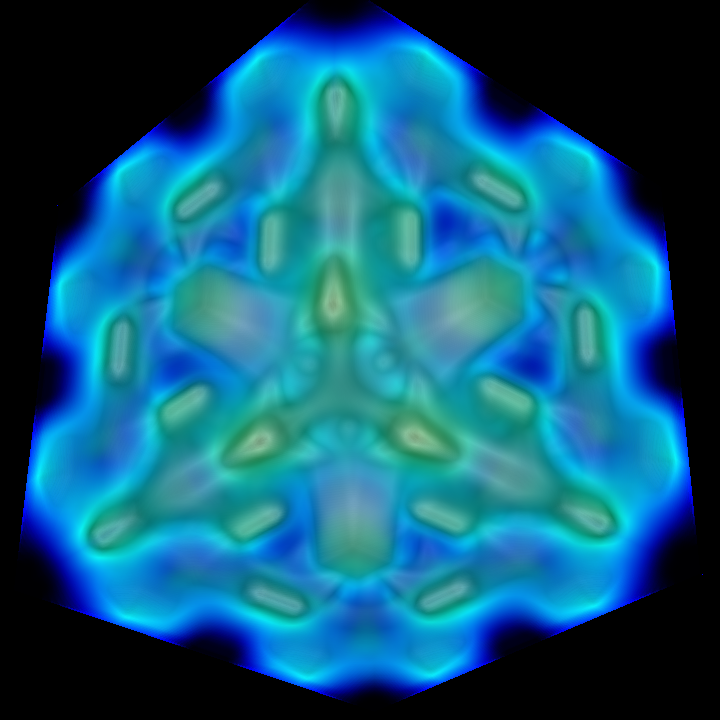
\includegraphics[width=\textwidth]{pictures/DVR2.png}
			\subcaption{}
			\label{SamplingPoints2}
		\end{subfigure}
	\end{minipage}
	\caption{Zwei Raycastings desselben Skalarfeldes mit unterschiedlichen Abtastraten.}
	\label{SamplingPoints}
\end{figure}

Die Qualit\"at eines Raycastings ist stark abh\"angig von der Abtastrate auf den Strahlen und somit vom Abstand zwischen den Abtastpunkten. Ein geringerer Abstand f\"uhrt generell zu weniger Artefakten und macht kleine Strukturen besser erkennbar, erh\"oht jedoch den Rechenaufwand. Indem der Nutzer die Abtastrate selbst ausw\"ahlt, kann er den Tradeoff zwischen Rechenzeit und Bildqualit\"at an seine Bed\"urfnisse anpassen, genau wie schon beim Texture Slicing. In \cref{SamplingPoints1,SamplingPoints2} sind zwei Darstellungen desselben Skalarfeldes $f:\mathbb{R}^3\rightarrow\mathbb{R}, f(x, y, z)=cos(x\cdot y\cdot z)$ zu sehen, die durch Raytracing mit einer unterschiedlichen Anzahl von Abtastpunkten erzeugt wurden. \cref{SamplingPoints1} wurde mit 20 Abtastpunkten erstellt, wodurch visuelle, scheibenartige Artefakte entstanden. Bei einer h\"oheren Menge von 200 Abtastpunkten in \cref{SamplingPoints2} verschwinden diese Artefakte.

\subsection{Cell Projection}
\begin{figure}
	\centering
	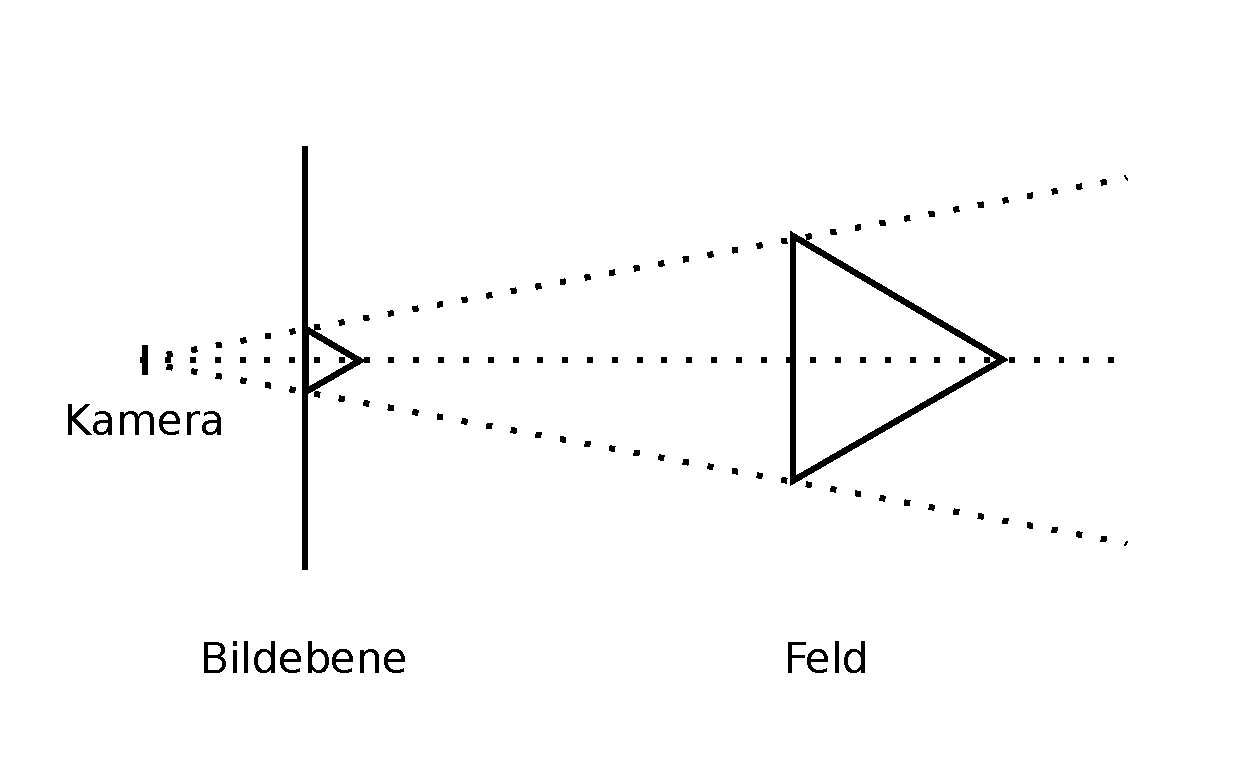
\includegraphics[width=0.6\textwidth]{pictures/CellProjection}
	\caption{Schematische Darstellung von Cell Projection. Das gro{\ss}e Dreieck rechts wird auf die Bildebene links projiziert. Die Projektion wird durch das kleinere Dreieck direkt an der Bildebene dargestellt.}
	\label{CellProjection}
\end{figure}
Cell Projection z\"ahlt zu den \textit{object-order} Verfahren. Es basiert auf der Arbeit von Lenz, Gudmundsson, Lindskog und Danielsson \cite{lenz86display} sowie der von Frieder, Gordon und Reynolds \cite{frieder1985back}. Die grundlegende Idee der Cell Projection besteht darin, f\"ur jedes Voxel ein zweidimensionales Polygon zu berechnen und dieses auf die Bildebene zu projizieren. Form, Farbe und Transparenz des Polygons werden dabei durch die Form des Voxels sowie die relative Position der Kamera zum Voxel bestimmt. Punkte innerhalb des Polygons sind Projektionen von Geraden durch das Voxel, deren Richtung von der Kameraposition abh\"angt. Die Opazit\"at an diesen Punkten entspricht dem Integral der Opazit\"at entlang der Linien. Dieses Vorgehen ist vergleichbar mit dem schon vorgestellten Continuous Scatterplotting, speziell dem \textbf{Fall 5}. In \cref{CellProjection} ist das Vorgehen schematisch abgebildet. Auf jeden Punkt der Bildebene wird ein eindimensionaler Ausschnitt des Voxels abgebildet. Die L\"ange dieses Ausschnitts gibt die Dicke des Voxels in Richtung des Punkts auf der Bildebene an, betrachtet von der Kameraposition aus. Diese Dicke wird in \cref{CellProjection} durch die Entfernung der Punkte auf den Schenkeln des Dreiecks zur Bildebene ausgedr\"uckt.

Wenn sich mehrere Projektionen der Voxel auf der Bildebene \"uberschneiden, werden sie mittels Blending kombiniert. Die f\"ur das Blending verwendeten Formeln sind abh\"angig von der Reihenfolge, in der die Voxel verarbeitet werden: Die \cref{front-to-back-color,front-to-back-alpha} im front-to-back Fall und die \cref{back-to-front-color,back-to-front-alpha} im back-to-front Fall. Bei \textit{object-order} Verfahren ist in der Regel keine fr\"uhzeitige Terminierung m\"oglich. Aus diesem Grund und weil back-to-front die akkumulierte Opazit\"at nicht abspeichern muss, wird es meistens bevorzugt.

\begin{figure}
	
\end{figure}

\begin{figure}			
	\begin{subfigure}{0.25\textwidth}
		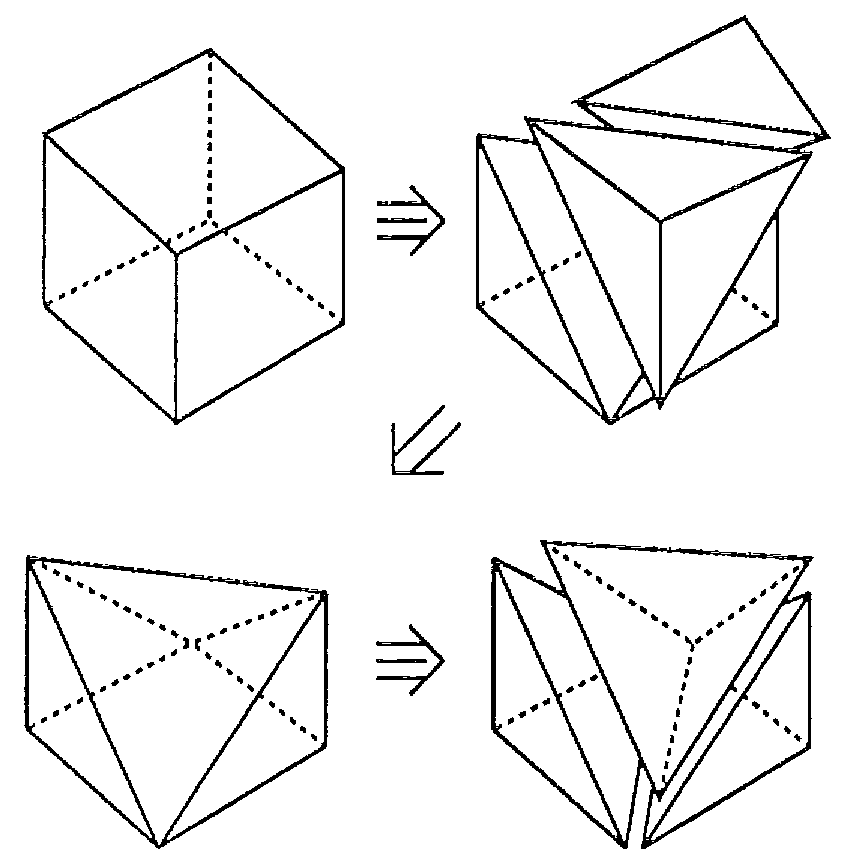
\includegraphics[width=\textwidth]{pictures/Split.png}
		\subcaption{}
		\label{Split}
	\end{subfigure}
	\begin{subfigure}{0.3\textwidth}
		\centering
		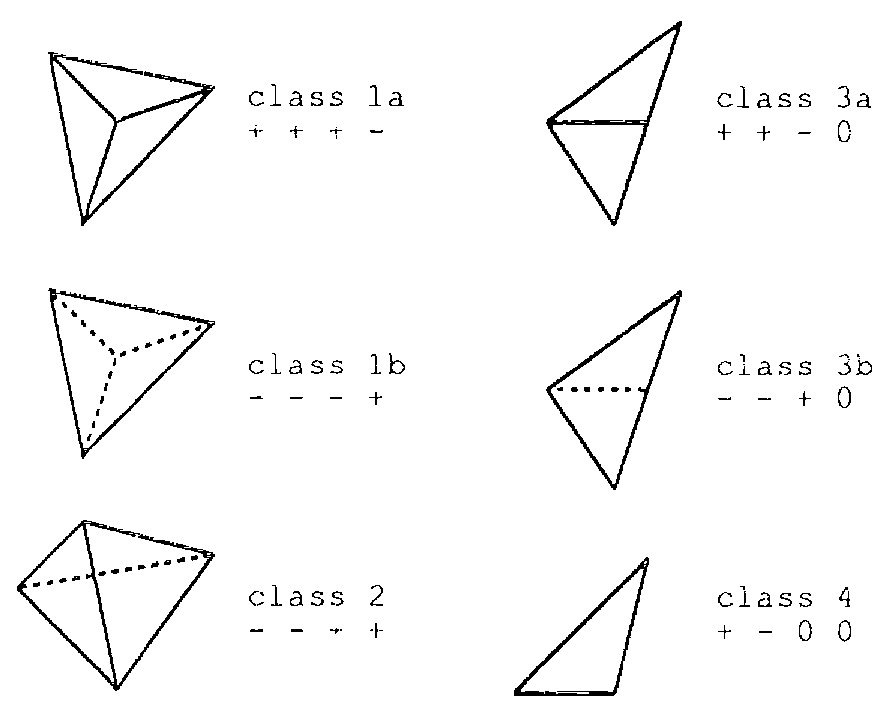
\includegraphics[width=\textwidth]{pictures/Classes.png}
		\subcaption{}
		\label{Classes}
	\end{subfigure}
	\begin{subfigure}{0.3\textwidth}
		\centering
		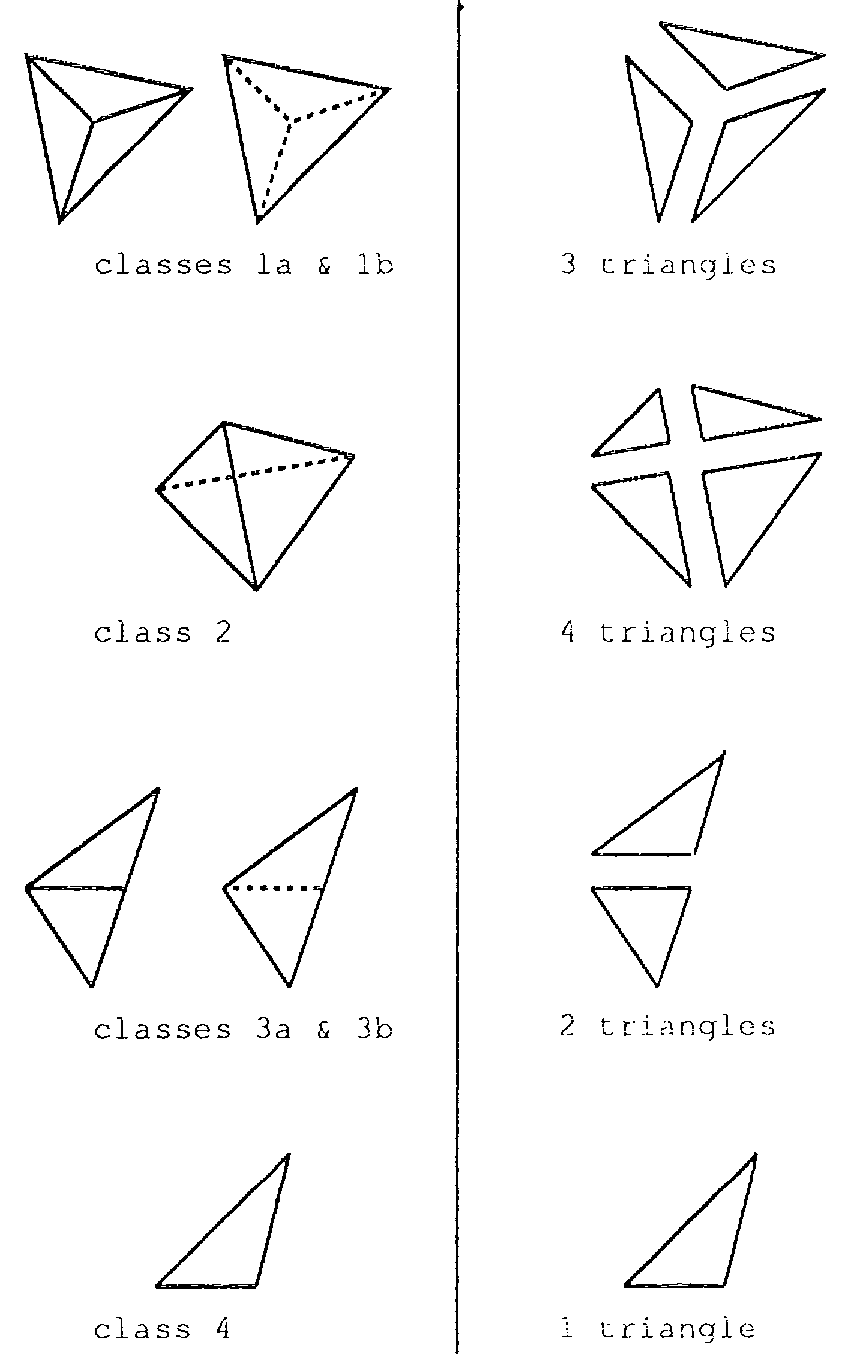
\includegraphics[width=\textwidth]{pictures/Triangle.png}
		\subcaption{}
		\label{Triangle}
	\end{subfigure}
	\caption{Teilaufgaben einer beispielhaften Cell Projection: (a) Zerlegung eines quaderf\"ormigen Voxels in f\"unf tetraedrische Voxel. (b) Klassifizierung von Tetraeder abh\"angig von ihrer Ausrichtung zur Kamera. (c) Zerlegung der Projektion des Tetraeders in Dreiecke.}
\end{figure}

Cell Projection Verfahren unterscheiden sich stark darin, welche Arten von Voxel als Eingabe dienen k\"onnen und wie die Umwandlung in zweidimensionale Voxel ausgef\"uhrt wird. Diese beiden Teilprobleme werden im Folgenden anhand des von Shirley und Tuchman \cite{shirley1990polygonal} entwickelten Algorithmus erl\"autert.

Im ersten Schritt zerlegt der Algorithmus die Voxel in disjunkte tetraedrische Teile (siehe \cref{Split}). Die daraus entstehenden Tetraeder werden anhand der Ausrichtung ihrer Fl\"achen zur Blickrichtung der Kamera klassifiziert. Dazu wird das Skalarprodukt zwischen den Normalen der Fl\"achen (die hier immer als nach au{\ss}en zeigend angenommen werden) und der Blickrichtung berechnet. Die Klassen sind in \cref{Classes} dargestellt. Die +, - und 0 neben den Klassen geben dabei an, welche Werte die Skalarprodukte jeweils annehmen k\"onnen: Ein + steht f\"ur ein positives, ein - f\"ur ein negatives Skalarprodukt. 0 steht daf\"ur, dass das Skalarprodukt 0 ist, also die Normale orthogonal zur Blickrichtung.

Nachdem die Tetraeder klassifiziert sind, werden die von ihnen durch Projektion auf die Bildebene erzeugten Fl\"achen bestimmt. Dazu werden die Eckpunkte projiziert und die entstehenden Polygone in Dreiecke zerlegt (siehe \cref{Triangle}). Werte f\"ur neu entstandene Eckpunkte der Dreiecke werden durch Interpolation berechnet. Die Dicke des Tetraeders an Punkten im Inneren des Polygons wird durch die Euklidische Distanzformel bestimmt. Die Opazit\"at an diesen Punkten wird abh\"angig von der Dicke des Tetraeders und den skalaren Werten entlang der Geraden durch den Tetraeder, die auf den Punkt abgebildet wird, bestimmt.

Schlussendlich werden die Dreiecke auf die Bildebene gerendert. Die Farb- und Opazit\"atswerte im Inneren der Dreiecke ergeben sich durch Interpolation der Werte an ihren Eckpunkten. 

Der Vorteil der Cell Projection liegt in der sehr exakten Darstellung des Datensatzes: Alle Voxel werden in korrekter Form und mit korrekten Dichtewerten gerendert, was bei den meisten anderen \textit{object-order} Verfahren nicht der Fall ist. Diese Exaktheit wird durch zus\"atzliche Vorberechnungen erreicht, die die Gesamtrechenzeit des Algorithmus erh\"ohen. Zudem k\"onnen die harten Kanten der projizierten Polygone visuelle Artefakte erzeugen, die bei anderen \textit{object-order} Verfahren nicht vorkommen.

\subsection{Splatting}

\begin{figure}
	\centering
	\begin{tikzpicture}
	
	
	\draw(-2.5,0) node{\Large$\frac{1}{273}$};
	\matrix (mtr) [matrix of nodes,row sep=-\pgflinewidth, nodes={draw, minimum width=0.7cm, minimum height=0.7cm}]
	{
		1 & 4 & 7 & 4 & 1\\
		4 & 16 & 26 & 16 & 4\\
		7 & 26 & 41 & 26 & 7\\
		4 & 16 & 26 & 16 & 4\\
		1 & 4 & 7 & 4 & 1\\
	};
	\end{tikzpicture}
	\caption{Ein diskreter $5\times5$ Gau{\ss} Kern. Die Werte in den Zellen werden mit dem Faktor links multipliziert, sodass die Summe aller Zellen 1 entspricht.}
	\label{kernel}
\end{figure}

Splatting basiert auf einem von Westover entwickelten Algorithmus\cite{westover1990footprint,westover1989interactive}. Wie auch bei der Cell Projection werden f\"ur die Voxel in back-to-front Reihenfolge zweidimensionale Repr\"asentationen gebildet, die auf die Bildebene projiziert und dort mittels Blending kombiniert werden. Im Gegensatz zur Cell Projection wird jedoch nicht versucht den Datensatz so exakt wie m\"oglich darzustellen, sondern das urspr\"ungliche Feld aus den diskreten Werten der Voxel so gut wie m\"oglich zu rekonstruieren und darzustellen. 

In der Signalverarbeitung ist die Rekonstruktion von kontinuierlichen Funktionen aus diskreten Funktionen ein zentrales Problem. Die Erzeugung einer diskreten Ann\"aherung an das urspr\"ungliche kontinuierliche Feld kann durch Faltung der diskreten Abtastung mit einem diskreten Kern geschehen. Daf\"ur werden eine Reihe unterschiedlicher Kerne benutzt. Einer der am meisten verwendeten ist die diskrete Abtastung von Gau{\ss}schen Glockenkurven. Splatting bedient sich dieser Technik, indem es die Projektion der Mittelpunkte der Voxel auf der Bildebene berechnet und diskrete Abtastungen von zweidimensionalen Glockenkurven an diesen platziert. Die Abtastungen werden abh\"angig von Eigenschaften der Voxel skaliert: Ihre Gr\"o{\ss}e, Form und Drehung werden so angepasst, dass sie die Form des Voxels so gut wie m\"oglich wiedergeben. Zus\"atzlich wird die H\"ohe des Maximums so skaliert, dass sie dem Wert des Voxels entspricht. Damit nicht f\"ur jeden Voxel ein neuer Kern berechnet werden muss, wird zu Beginn des Rendering ein einzelner Filterkern berechnet und in einer Lookup-Tabelle abgespeichert. Eine solche Tabelle ist in \cref{kernel} dargestellt.

Splatting bietet gegen\"uber der Cell Projection und \"ahnlichen Verfahren den Vorteil, dass im entstehenden Bild keine harten Voxelkanten zu sehen sind. Die aus der Signalverarbeitung \"ubernommenen Methoden garantieren eine hohe Bildqualit\"at mit relativ kurzen Rechenzeiten. Splatting ist daher eines der beliebtesten \textit{object-order} Verfahren.
Das Fehlen von harten Kanten stellt jedoch auch einen Nachteil von Splatting dar: Die Grenzen des Datensatzes werden weich gezeichnet. Ein zus\"atzliches Problem tritt auf, wenn die Gr\"o{\ss}e der Voxel stark variiert. Wenn beispielsweise einige wenige Voxel sehr viel gr\"o{\ss}er sind als der Rest, k\"onnen die f\"ur diese Voxel erzeugten Kerne deutlich erkennbar sein. Da einzelne Kerne die Form ihrer Voxel nur schlecht wiedergeben k\"onnen, kann dies zu deutlichen visuellen Artefakten im erzeugten Bild f\"uhren.

\subsection{Shear Warp}
\begin{figure}
	\centering
	\begin{subfigure}{0.49\textwidth}
		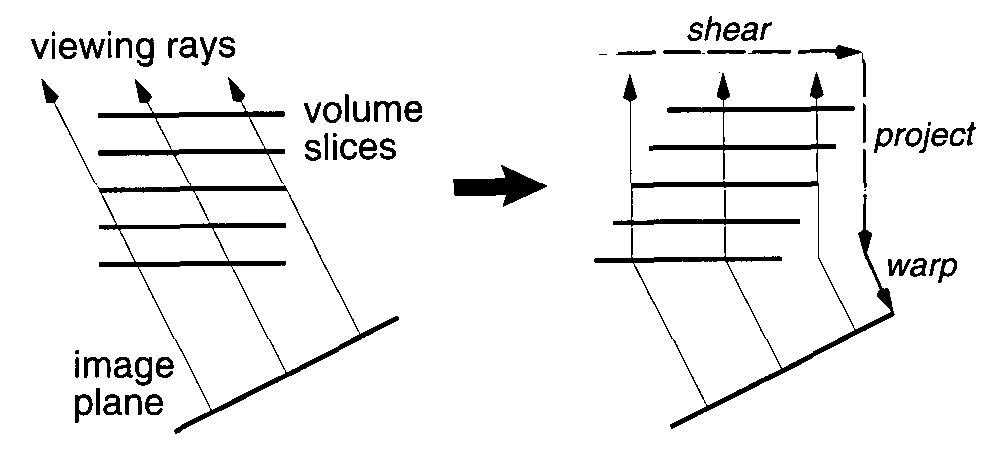
\includegraphics[width=\textwidth]{pictures/ShearWarp1}
		\caption{}
		\label{ShearWarp1}
	\end{subfigure}
	\hfill
	\begin{subfigure}{0.49\textwidth}
		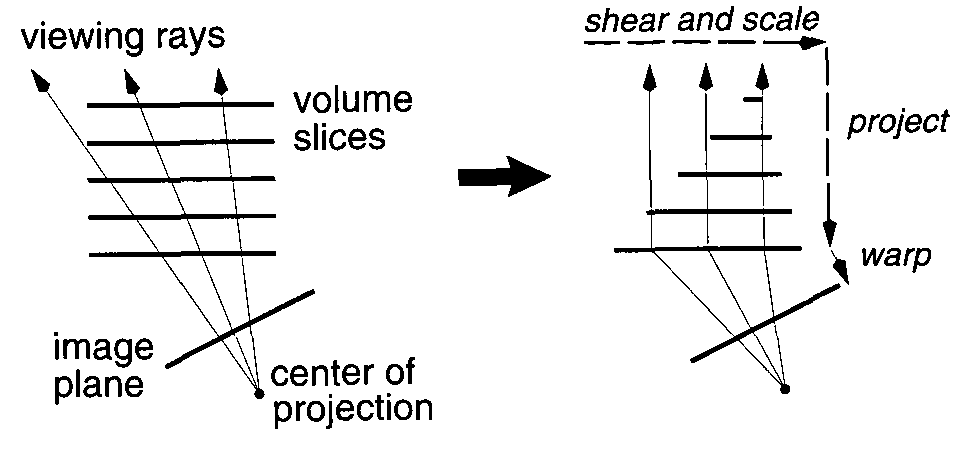
\includegraphics[width=\textwidth]{pictures/ShearWarp2}
		\caption{}
		\label{ShearWarp2}
	\end{subfigure}
	\caption{Darstellungen der im Shear Warp verwendeten Scherungs- und Verzerrungsoperationen auf dem Datensatz und den Sichtstrahlen in (a) paralleler Projektion und (b) perspektivischer Projektion. Entnommen aus \cite{lacroute1994fast}.}
\end{figure}
Shear Warp z\"ahlt zu den \textit{hybriden} Verfahren. Es kombiniert Techniken aus \textit{object-} und \textit{image-order} Verfahren, wodurch es typische Vorteile beider Arten bietet. Entwickelt wurde Shear Warp von Philipp Lacroute und Marc Levoy, die es 1994 zuerst vorstellten\cite{lacroute1994fast}. 

Der Grundansatz des Shear Warp besteht darin, den volumetrischen Datensatz mittels einer Scherung (engl. \glq shear\grq{}) so zu transformieren, dass von der Kameraposition ausgehende und die Bildebene schneidende Strahlen parallel zu einer der Koordinatenachsen sind. Welche Koordinatenachse daf\"ur gew\"ahlt wird h\"angt von Blickrichtung der Kamera ab, in der Regel wird die Koordinatenachse mit dem geringsten Winkel zur Blickrichtung bevorzugt. Im Folgenden wird diese Achse als \glq Sichtachse\grq{} bezeichnet, die zugeh\"orige Koordinate \glq Sichtkoordinate\grq{}. 

Abh\"angig von der Art der sp\"ater verwendeten Projektion muss die Scherung unterschiedlich durchgef\"uhrt werden. Bei paralleler Projektion gen\"ugt eine Verschiebung der Voxelschichten untereinander (siehe \cref{ShearWarp1}). Dies setzt voraus, dass die Voxel eine einheitliche Gr\"o{\ss}e und Form haben, in der Regel quaderf\"ormig. Bei perspektivischer Projektion muss zus\"atzlich die Gr\"o{\ss}e der Schichten so skaliert werden, dass sie mit zunehmender Entfernung zur Kamera kleiner werden (siehe \cref{ShearWarp2}). Wenn durch Verschiebung und Skalierung mehrere Eingabevoxel zum Teil oder ganz auf einen Ausgabevoxel abgebildet werden, m\"ussen die Werte der Voxel gewichtet nach der Gr\"o{\ss}e des Anteils interpoliert werden, um den Datensatz so gut wie m\"oglich darstellen zu k\"onnen.

\begin{figure}
	\centering
	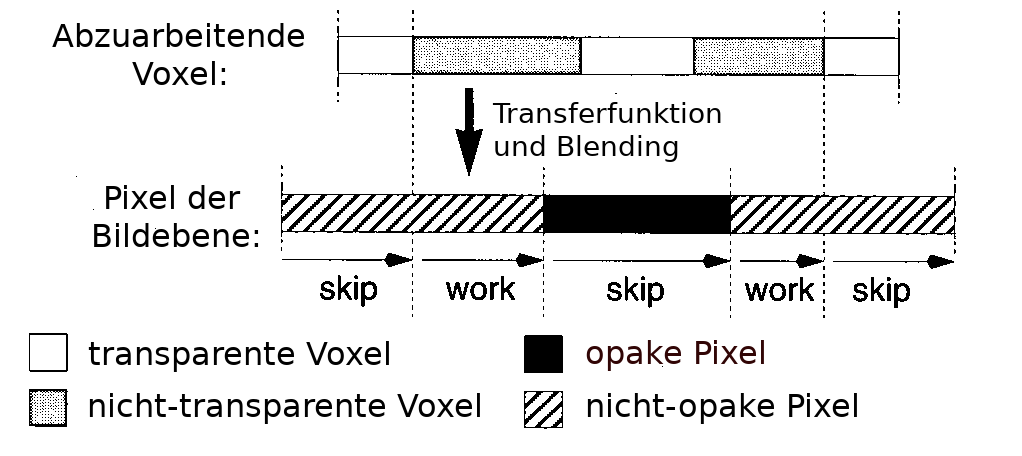
\includegraphics[width=0.7\textwidth]{pictures/Scanline.png}
	\caption{Darstellung der optimierten Abbildung von Voxeln auf Pixel. Wenn entweder die Voxel vollst\"andig transparent oder die Zielpixel vollst\"andig opak sind, werden sie \"ubersprungen (\glq skip\grq{}), ansonsten werden die Voxelwerte auf die Pixel abgebildet (\glq work\grq{}). Erstellt nach einem Bild aus \cite{lacroute1994fast}.}
	\label{Scanline}
\end{figure}

Nachdem die Scherung durchgef\"uhrt wurde, wird die Projektion der Voxel auf die Bildebene begonnen. Der Datensatz wird dabei schichtweise verarbeitet. Die Pixel, auf die ein Voxel abgebildet wird, sind durch die Scherung leicht zu bestimmen. Es sind genau die, deren zwei Koordinaten innerhalb des Grenzen des projizierten Voxels liegen. Dies erspart teure Projektionsoperatoren wie bei \textit{object-order} oder schrittweise Abtastung wie bei \textit{image-order} Verfahren. Diese Eigenschaft erlaubt eine zus\"atzliche Optimierung. Wenn ein Pixel der Bildebene bereits eine hohe Opazit\"at akkumuliert hat (\"ahnlich wie die fr\"uhzeitige Terminierung bei \textit{image-order} Verfahren), kann dieser \"ubersprungen werden. Implementiert wird dies meistens, indem f\"ur jedes opake Pixel der Offset zum n\"achsten nicht-opaken Pixel gespeichert wird. Das gleiche Verfahren kann auch bei Voxeln verwendet werden, denen die Transferfunktion eine Opazit\"at von 0, also vollst\"andige Transparenz, zuordnet. Diese enthalten den Offset zum n\"achsten Voxel mit Opazit\"at gr\"o{\ss}er 0. \cref{Scanline} zeigt diese Optimierung. Die notwendigen Offsets der transparenten Voxel werden f\"ur jede achsenparallele Blickrichtung vorberechnet, also insgesamt dreimal. Optional k\"onnen komplett transparente Voxel auch direkt entfernt und die Offsets in den nicht-transparenten Voxeln gespeichert werden, wodurch sich die bei \textit{object-order} Verfahren \"ublichen Speicherersparnisse ergeben. 

Im Gegensatz zu \textit{object-order} Verfahren werden Voxel beim Shear Warp nicht in Basisfunktionen \"ubersetzt, sondern pro Pixel die jeweiligen Werte durch Interpolation bestimmt. Da die Dicke der Voxel von der Blickrichtung abh\"angt, wird die Opazit\"at mittels einer vorberechneten Tabelle skaliert. Im perspektivischen Fall kann es sein, dass auf einen Pixel zwei oder mehr Voxel abgebildet werden. Dies muss bei der Optimierung ber\"ucksichtigt werden.

Zum Abschluss wird eine zur Scherung inverse Verzerrung auf die Bildebene angewendet (engl. \glq warp\grq{}), um das endg\"ultige Bild zu erzeugen. Diese Operation ist, wie in \cref{ShearWarp1,ShearWarp2} dargestellt, identisch f\"ur parallele und perspektivische Projektion.

\subsection{Wahl des DVR-Verfahrens}
Die vorgestellten Verfahren unterscheiden sich in Hinsicht auf Laufzeit, Speicherverbrauch, Adaptierbarkeit und Qualit\"at der erzeugten Visualisierung. Zum Abschluss des Kapitels werden sie deshalb anhand dieser Eigenschaften und den aus der Aufgabenstellung resultierenden Anforderungen verglichen und eins der Verfahren zur Umsetzung ausgew\"ahlt.

Object-order Verfahren bieten im Allgemeinen die Vorteile geringen Speicherverbrauchs und relativ geringer Laufzeit. Diese Vorteile werden jedoch durch eine Reihe von Nachteilen erkauft, die sie f\"ur die vorliegende Arbeit ungeeignet machen:


\paragraph{Visuelle Artefakte} Aufgrund der typischen Formen der Basisfunktionen sind \textit{object-order} Verfahren anf\"allig f\"ur die Erzeugung visueller Artefakte. Bei Datens\"atzen mit Voxeln gleichm\"a{\ss}iger Gr\"o{\ss}e sind die Artefakte meist nicht wahrnehmbar. Wenn einzelne Voxel deutlich gr\"o{\ss}er sind, werden auch die Basisfunktionen sichtbar, womit auch die Sichtbarkeit der Artefakte zunimmt. Durch die Transformation von Voxeln in die Invariantenr\"aume k\"onnen sehr gro{\ss}e Voxel entstehen, weshalb eine Vorverarbeitung und Zerst\"uckelung solcher Voxel notwendig werden w\"urde.

\paragraph{Teilweise Darstellung von Voxeln} Die Anforderungen spezifizieren Interaktionen, durch die Teile des Invariantenraumes und die diesen Teilen entsprechenden Teile des Objektes ausgeblendet werden. Um dies mit \textit{object-order} Verfahren zu implementieren, m\"ussen komplexe Operationen auf die Basisfunktionen angewendet werden, was die Laufzeit wahrscheinlich deutlich erh\"ohen w\"urde.

\paragraph{Keine fr\"uhzeitige Terminierung} Durch die Anwendung der Prinzipien des Continuous Scatterplotting entstehen m\"oglicherweise Gebiete mit hoher Dichte. Da \textit{object-order} Verfahren im Allgemeinen keine fr\"uhzeitige Terminierung unterst\"utzen, kann dies nicht ausgenutzt werden um die Laufzeit zu verbessern.

Das Problem der teilweisen Darstellung von Voxeln tritt auch bei Shear Warp auf, weshalb es nicht ohne aufw\"andige \"Uberarbeitung und mit erh\"ohter Laufzeit verwendet werden konnte.

Damit verbleiben als Optionen nur noch die \textit{image-order} Verfahren. Unterschiede zwischen diesen lassen sich meistens auf einen Tradeoff zwischen Rechenzeit und Bildqualit\"at zur\"uckf\"uhren. Raycasting bietet dabei eine M\"oglichkeit f\"ur den Benutzer diesen Tradeoff selbst zu beeinflussen und, falls entsprechend eingestellt, die besten Ergebnisse. Auch die teilweise Darstellung von Voxeln ist leicht in Raycasting zu implementieren, indem die Werte der Invarianten an Abtastpunkten interpoliert werden und Punkte mit Werten au{\ss}erhalb des gew\"ahlten Bereichs \"ubersprungen werden. Daher wird f\"ur diese Arbeit Raycasting als DVR-Verfahren gew\"ahlt.



\section{Umsetzung}
\label{sec:Umsetzung}
In diesem Kapitel wird beschrieben, wie die Grundlagen, Technologien und Verfahren aus den vorherigen Kapiteln eingesetzt wurden, um eine interaktive Tensorfeldvisualisierung in FAnToM zu erzeugen.

Die Grundidee der entwickelten Visualisierung besteht darin, zwei DVR zu erzeugen. Das Erste stellt die Zellen des urspr\"unglichen Feldes dar, \"uber die eine konstante Dichte angenommen wird. Da das Zielgebiet der Anwendung die Materialforschung ist, wird das urspr\"ungliche Feld im Ortsraum im Folgenden als \glq Objekt\grq{} bezeichnet. F\"ur das zweite DVR werden die 3 Invarianten eines Invariantensatzes der an den Eckpunkten der Zellen definierten Tensoren berechnet und diese als Koordinaten interpretiert. Die Zellstruktur wird somit in einen \glq Invariantenraum\grq{} \"uberf\"uhrt. Wegen der Popularit\"at der K- und R-Invariantens\"atze werden die Koordinaten optional in ein zylindrisches Koordinatensystem \"ubertragen. Die Dichten in den Zellen der neuen Zellstruktur werden durch Methoden des Continuous Scatterplotting berechnet.

Das Verfahren zur Erzeugung der Darstellungen und Interaktionen ist im Folgenden n\"aher erl\"autert.

\subsection{Umsetzung des Continuous Scatterplotting}
\label{CSPImplementation}
Um ein vollst\"andiges Continuous Scatterplotting zu implementieren, m\"ussen drei Teilaufgaben erf\"ullt werden.

Als Erstes m\"ussen die Volumen der Tetraeder im Orts- und Invariantenraum berechnet werden. Aus der Volumen\"anderung der Zellen bei der Abbildung vom Orts- in den Invariantenraum  lassen sich die Dichten $\sigma_{V_i}$ der Tetraeder $V_i$ im Invariantenraum bestimmen. Dabei wird die f\"ur \textbf{Fall 1} angegebene \cref{Case1Formula} verwendet. Die anderen F\"alle k\"onnen zwar theoretisch vorkommen, sind jedoch extrem unwahrscheinlich. Durch unvermeidbare Rundungsfehler werden Bereiche konstanter Invarianten (\textbf{Fall 2}), Nullmengen (\textbf{Fall 3}) und Abbildungen auf Teilr\"aume mit geringerer Dimension (\textbf{Fall 5}) zerst\"ort. Das Erkennen von diesen Rundungsfehlern wird dadurch erschwert, dass in den verwendeten Datens\"atzen tats\"achlich Bereiche mit sehr geringen Ver\"anderungen der Invarianten oder Abbildungen auf sehr flache Tetraeder vorkommen. Die Unterscheidung zwischen solchen extremen Formen von \textbf{Fall 1} und den anderen F\"allen ist nicht ohne Weiteres m\"oglich. \textbf{Fall 4} kommt nicht vor, da die verwendeten Felder \"uberall differenzierbar sind.

Als zweites m\"ussen die Dichtewerte in Bereichen in denen sich mehrere Zellen \"uberlappen korrekt berechnet werden. Da die $V_i$ eine vollst\"andige Zerlegung des Feldes darstellen, l\"asst sich \cref{DensitySum} anwenden. Die $\sigma_V$ entsprechen den berechneten Dichtewerten pro Tetraeder, die f\"ur jedes Voxel durch das Blending aufaddiert werden. Das Abspeichern der Ergebnisse dieser Teilaufgabe ist nicht trivial, da ihre Form dem Schnittraum beliebig vieler Tetraeder entsprechen kann.

Und als drittes muss das Continuous Scatterplotting in ein Format transformiert werden, das als Eingabe des sp\"ater implementierten Raycastings dienen kann. Um Rechenzeit zu sparen sollte versucht werden, Teilaufgabe 2 und 3 zu kombinieren.


\subsection{Datenvorbereitung}
\begin{figure}
	\centering
	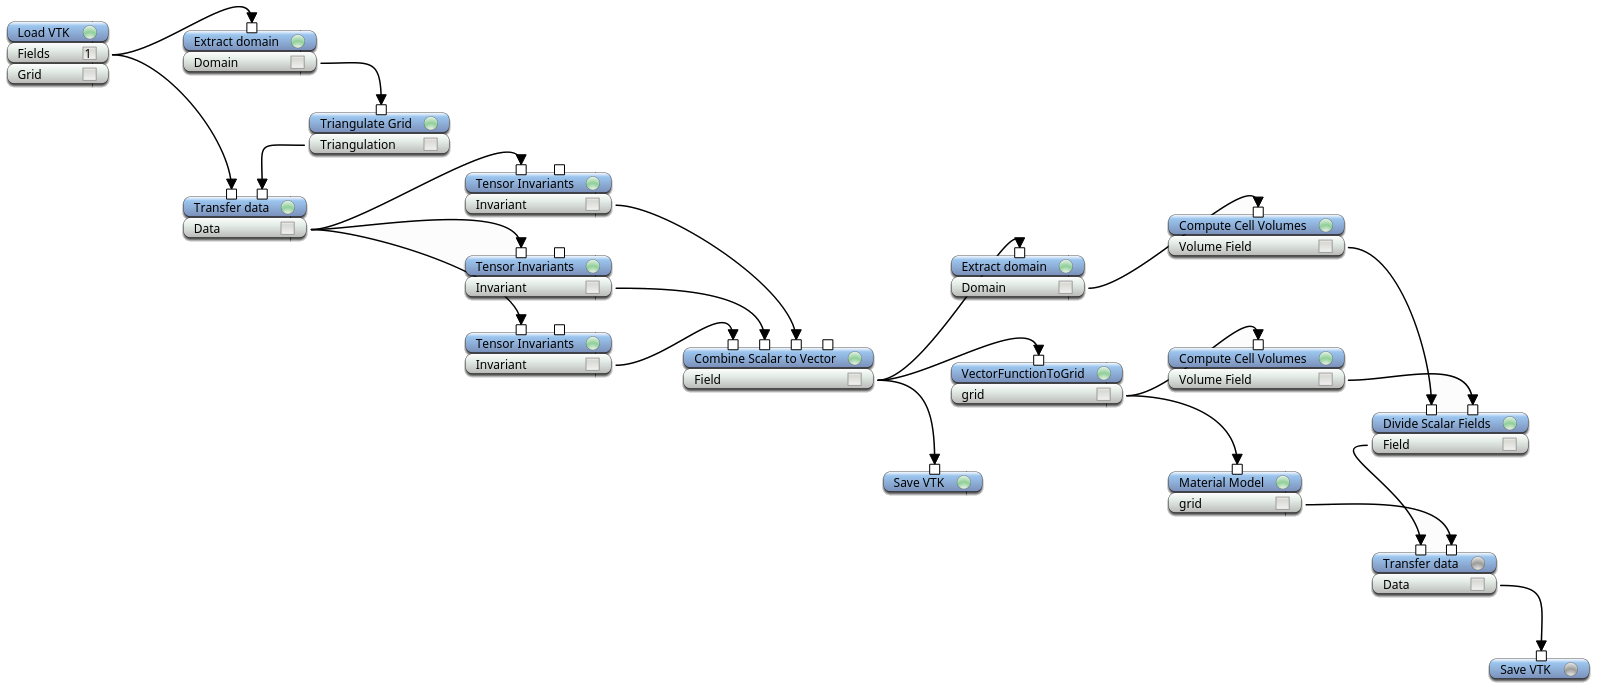
\includegraphics[width=\textwidth]{pictures/BigSession.png}
	\caption{Der Flowgraph der FAnToM Session, die zur Vorbereitung der Daten verwendet wird.}
	\label{BigSession}
\end{figure}

\subsubsection{Die Vorbereitungssession}
\label{sec:Vorverarbeitung}
Bevor die Visualisierung beginnen kann, m\"ussen die Daten vorbereitet werden. Um Zeit zu sparen, wird dieser Schritt f\"ur jeden Datensatz nur einmal durchgef\"uhrt und die Ergebnisse abgespeichert. Ein Screenshot der f\"ur die Datenvorbereitung verwendeten Session ist in \cref{BigSession} zu sehen. Die in der Vorbereitungssession durchgef\"uhrten Berechnungen sind im folgenden kurz beschrieben. Die verantwortlichen Algorithmen werden in Klammern angegeben. Fast alle der verwendeten Algorithmen sind standardm\"a{\ss}ig in FAnToM vorhanden. Die restlichen 3, \glq VectorFunctionToGrid\grq{}, \glq CylindricalCoordinates\grq{} und \glq Divide Scalar Fields\grq{}, sind sehr einfache Algorithmen, die f\"ur die vorliegende Arbeit implementiert wurden.

Die im VTK Format\cite{avila2010vtk} vorliegenden Daten werden geladen (\glq Load/VTK\grq{}) und die Zellstruktur, auf der das Feld definiert ist, tetraedrisiert (\glq Extract Domain\grq{}, \glq Triangulate Grid\grq{} und \glq Transfer Data\grq{}). Die Invarianten der Tensoren an den Eckpunkten der Zellen werden berechnet und zu einem Vektorfeld kombiniert (\glq Tensor Invariants\grq{} und \glq Combine Scalar to Vector\grq{}). Eine Kopie dieses Vektorfeldes wird abgespeichert (\glq Save VTK\grq{}), um als erste Eingabe der Visualisierungssession zu dienen. Indem das Vektorfeld als Koordinaten der Punkte interpretiert wird, wird eine Kopie der Zellstruktur im Invariantenraum erzeugt (\glq Vector Function To Grid\grq{}). Optional k\"onnen f\"ur Invarianten, die sich gut in zylindrischen Koordinaten darstellen lassen, die Punkte als zylindrische Koordinaten interpretiert und in kartesische Koordinaten umgerechnet werden (\glq Cylindrical Coordinates\grq{}). Dadurch wird eine einheitliche Darstellung des Datensatzes in kartesischen Koordinaten f\"ur die Visualisierungssession geschaffen, wodurch Rechenzeit gespart werden kann. In jedem Fall werden die Volumen Zellen im Orts- und Invariantenraum berechnet (\glq Compute Cell Volumes\grq{}). Unter der Annahme, dass die Dichten innerhalb der Zellen im Ortsraum konstant 1,0 waren, ergeben sich die Dichten im Invariantenraum als Quotient der Volumen im Ortsraum und der im Invariantenraum (\glq Divide Scalar Fields\grq{}). Am Ende werden die berechneten Dichtewerte der Zellstruktur im Invariantenraum zugewiesen und das Ergebnis abgespeichert, um als zweite Eingabe der Visualisierunssession zu dienen.

\subsubsection{Die Visualisierungssession}
\begin{figure}
	\centering
	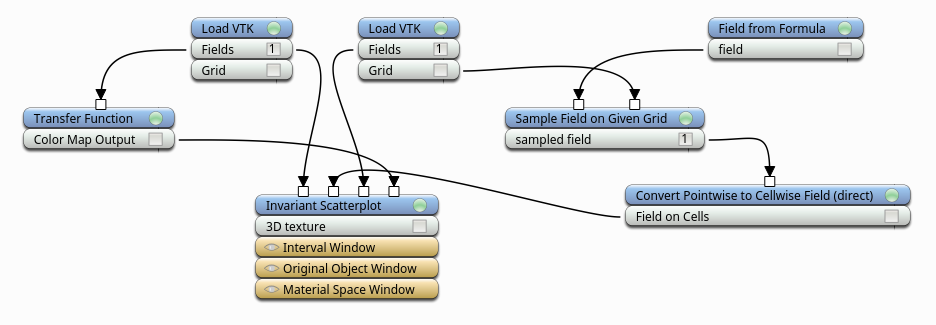
\includegraphics[width=0.8\textwidth]{pictures/VisSession.png}
	\caption{Der Flowgraph der Visualisierungssession.}
	\label{VisualizationSession}
\end{figure}

Zwei Teile der Datenvorbereitung m\"ussen in der gleichen Session stattfinden wie die Visualisierung selbst, um dem Anwender die M\"oglichkeit der Interaktion zu geben. Das sind zum einen die Erzeugung der Transferfunktion, zum anderen die Berechnung der Dichte innerhalb der Voxel im Objekt. Die Session ist in \cref{VisualizationSession} zu sehen.

Der linke \glq VTK Load\grq{} Algorithmus l\"adt dabei das skalare Dichtefeld im Invariantenraum, der rechte das Vektorfeld auf den urspr\"unglichen Punkten, in dem die Invarianten gespeichert sind. Vom Algorithmus \glq Transfer Function\grq{} wird eine Transferfunktion f\"ur das Feld im Invariantenraum erzeugt. Wie in \cref{Colormap} beschrieben, ist diese vom Nutzer frei konfigurierbar und wird in Echtzeit auf die Darstellung angewendet. Die Dichten der Voxel im Objekt werden durch eine Funktion bestimmt, die in den Algorithmus \glq Field from Formula\grq{} eingegeben wird (standardm\"a{\ss}ig konstant 1). Die geladenen VKT Dateien, die Transferfunktion und die neuen Voxeldichten werden am Ende dem Visualisierungsalgorithmus \"ubergeben

\subsection{Voxelisierung}
Um Teilschritte 2 und 3 des beschriebenen Verfahrens zur Umsetzung eines Continuous Scatterplotting zu implementieren, wird aus den Tetraedern mit den in der Vorverarbeitung berechneten Dichtewerten eine 3D Textur erzeugt. Eine 2D Textur kann im Allgemeinen als Tabelle aufgefasst werden, in der Farbwerte codiert sind. 3D Texturen setzen sich aus vielen 2D Texturen zusammen, deren Felder die Eigenschaften von Voxeln einer Schicht der 3D Textur beschreiben. 

Um die Tetraeder und ihre Dichtewerte durch Positionen und Eigenschaften von Voxeln zu repr\"asentieren, wird ein Verfahren implementiert, das f\"ur jedes Voxel die geschnittenen Tetraeder bestimmt und deren Dichtewerte auf die Dichte des Voxels aufaddiert. Dies wird als Voxelisierung bezeichnet. Initial ist die Dichte eines Voxels 0. FAnToM besitzt zwar eine effiziente Funktion, um Werte innerhalb der Zellen eines Feldes zu berechnen, diese ist jedoch nicht in der Lage, mit selbstdurchdringenden Feldern, wie sie bei der \"Uberf\"uhrung in den Invariantenraum entstehen k\"onnen, umzugehen. Es war deshalb notwendig, eine effiziente Methode zur Erzeugung der 3D Texturen zu implementieren. 

\begin{figure}
	\centering
	\hspace{0.5cm}
	\begin{subfigure}{0.2\textwidth}
		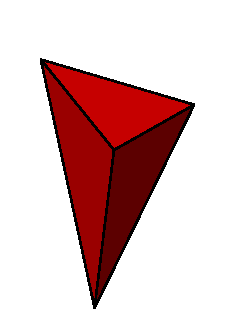
\includegraphics[width=0.9\textwidth]{pictures/TetraCuts1}
		\caption{}
	\end{subfigure}
	\hspace{1cm}
	\begin{subfigure}{0.2\textwidth}
		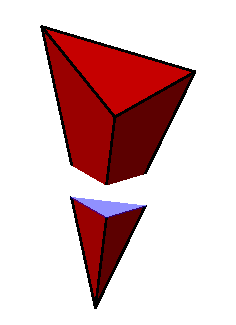
\includegraphics[width=0.9\textwidth]{pictures/TetraCuts2}
		\caption{}
	\end{subfigure}
	\hspace{1cm}
	\begin{subfigure}{0.2\textwidth}
		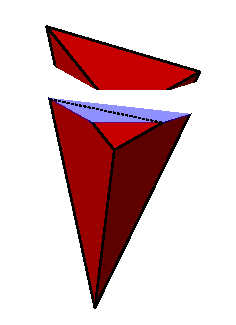
\includegraphics[width=0.9\textwidth]{pictures/TetraCuts3}
		\caption{}
	\end{subfigure}
	\hspace{0.5cm}
	\caption{Darstellungen von m\"oglichen Schnitten durch einen Tetraeder. (a) Der Tetraeder ohne Schnitte. (b) Ein Schnitt, der durch ein einzelnes Dreieck dargestellt werden kann. (b) Ein Schnitt, der ein Viereck bildet. Die gestrichelte Linie deutet eine m\"ogliche Unterteilung in Dreiecke an.}
	\label{TetraCuts}
\end{figure}

OpenGL stellt verschiedene Optionen f\"ur Farbcodierung zur Auswahl, womit Speicherbedarf und Pr\"azision eingestellt werden k\"onnen. F\"ur die vorliegende Arbeit wurde \glq GL\_RGBA16\grq{} gew\"ahlt, die vier Werte mit jeweils 16 Bit Pr\"azision zur Verf\"ugung stellt. \"Ublicherweise wird in einem Feld der Tabelle die Werte f\"ur den roten, gr\"unen und blauen Anteil der Farbe sowie die Transparenz (\glq Alpha\grq{}) an dieser Stelle codiert. Das DVR-Verfahren interpretiert diese Werte jedoch anders: Der Alphawert entspricht der Dichte und die restlichen drei Farbwerte den interpolierten Invarianten der Zelle, in der das Voxel liegt. Die Invarianten spielen allerdings nur bei der Visualisierung im Ortsraum eine Rolle, weshalb die Werte f\"ur Rot, Gr\"un und Blau in der Textur im Invariantenraum leer gelassen werden.

Aufgrund der leichten Parallelisierbarkeit bot es sich an, die Voxelisierung durch OpenGL und somit auf der Grafikkarte durchf\"uhren zu lassen. Das Verfahren basiert auf der Arbeit von Rueda et al.\cite{rueda2004voxelization}. Dabei werden Schichten der 3D Textur berechnet, indem die Schnittfl\"achen zwischen den Tetraedern und Ebenen bestimmt werden. Die Ebenen verlaufen dabei durch die Mittelpunkte der Voxel einer Schicht der Textur. Da der Schnitt zwischen einer Ebene und einem Tetraeder immer entweder ein Dreieck oder ein Viereck ist, kann er als Folge von einem oder zwei Dreiecken dargestellt werden (siehe \cref{TetraCuts}). Diese Dreiecke wiederum werden durch den standardm\"a{\ss}igen Rasterisierer von OpenGL in die fertigen Voxel unterteilt. Das komplette Verfahren ist in Form einer Shaderpipeline implementiert, die im Folgenden kurz erl\"autert wird. Falls der Shader nicht-triviale Algorithmen enth\"alt, ist zus\"atzlich der Algorithmus in vereinfachter Form angegeben.

Die Eingabe des Vertex-Shaders besteht aus den Punkten der Tetraeder, ihren jeweiligen Dichten und optional den an den Punkten berechneten Invarianten. OpenGL l\"asst allerdings in den von FAnToM unterst\"utzten Versionen keine Tetraeder als Eingabe zu. Deshalb m\"ussen diese auf eine andere Art \"ubergeben werden. Eine M\"oglichkeit dazu sind Liniensegmente mit Nachbarschaft (\glq GL\_LINES\_ADJACENCY\_EXT\grq{}). Das Format von Liniensegmenten mit Nachbarschaft besteht aus vier Punkten pro Primitive: Der erste Punkt entspricht dem Beginn des vorhergehenden Liniensegments, der zweite und dritte Punkt entsprechen dem aktuellen Liniensegment und der vierte Punkt ist der Endpunkt des n\"achsten Liniensegments. Da es immer genau vier Punkte pro Primitive gibt, eignet das Format sich auch, um Tetraeder an die Pipeline zu \"ubergeben.

Da die zylindrische Darstellung in Richtung der x-Achse sehr gro{\ss} werden kann, wurde ein Verfahren entwickelt und implementiert, das das Feld entlang der x-Achse unterteilt und in mehrere einzelne Texturen voxelisiert. Dasselbe Verfahren kann theoretisch auch f\"ur die anderen Richtungen implementiert werden, das war jedoch f\"ur keinen der verwendeten Datens\"atze n\"otig.

Wie schon im \cref{sec:OpenGL} angesprochen, ist es m\"oglich, die Ausgabe der Renderpipeline in einer Textur zu speichern. Dazu wird ein Framebuffer verwendet, der Schichten der 3D Textur als Ausgabe der Pipeline bindet. Die Voxelisierung wird also f\"ur jede Schicht einzeln durchgef\"uhrt.

Die Anzahl an Voxeln pro Dimension in der 3D Textur kann vom Nutzer selbst festgelegt werden. Falls in Richtung der x-Achse ein Wert \"uber 2048 gew\"ahlt wird, werden mehrere Texturen erzeugt. 2048 ist die in der von FAnToM verwendeten OpenGL Version die maximale Ausdehung einer 3D Textur in jede Richtung.

Eine wichtige Eigenschaft der Voxelisierung liegt darin, dass die Komplexit\"at des Datensatzes auf ein vom Benutzer festgelegtes Ma{\ss} reduziert wird. Unabh\"angig davon, aus wie vielen Zellen der zu visualisierende Datensatz besteht, wird immer die vom Benutzer vorgegebene Anzahl von Voxeln erzeugt. Dies bringt Vor- und Nachteile mit sich.

Zu den Vorteilen geh\"ort, dass die Voxelisierung nur ausgef\"uhrt werden muss, wenn neue Daten geladen werden oder sich Parameter der Voxelisierung selbst \"andern. Die Laufzeit des Raycastings ist ausschlie{\ss}lich abh\"angig von der Anzahl der einzuf\"arbenden Pixel und der Menge an Abtastpunkten pro Strahl. Durch diese beiden Eigenschaften ist es m\"oglich, auch sehr gro{\ss}e Datens\"atze explorativ zu analysieren, nachdem sie einmal voxelisiert wurden. Dadurch stellt die Voxelisierung einen wichtigen Ansatz dar, um \textbf{Herausforderung 2} aus der Einleitung, die Menge der Daten pro Datensatz, zu l\"osen.

Daf\"ur werden eine Reihe von Nachteilen in Kauf genommen. Ein Nachteil liegt darin, dass durch die Voxelisierung leicht Stufenartefakte entstehen. Dieser Effekt tritt im zweidimensionalen Fall h\"aufig auf und wird dort mit speziellen Verfahren abgemildert. Varianten dieser Verfahren im Dreidimensionalen k\"onnten m\"oglicherweise auch auf die 3D Texturen angewendet werden, dies ist jedoch im Verlauf der vorliegenden Arbeit noch nicht untersucht worden. Weitere Probleme treten auf, wenn Zellen sehr klein sind und dadurch nur auf wenige Voxel abgebildet werden. In diesem Fall gehen Informationen \"uber die Form der Zellen verloren.

Die Dichte innerhalb eines Voxels entspricht der Summe der Tetraeder die das Voxel schneiden, unabh\"angig davon, wie viel des Voxels vom Tetraeder eingenommen wird. Dadurch enth\"alt die 3D Textur insgesamt mehr Masse als das urspr\"ungliche Feld, was gegen einen Grundsatz des Continuous Scatterplotting, die Masseerhaltung, verst\"o{\ss}t. Eine M\"oglichkeit diesen Fehler zu reduzieren oder sogar komplett zu vermeiden w\"are es, pro Voxel die Dichtewerte an mehreren Punkten innerhalb des Voxels zu berechnen und die Dichte des Voxels auf den Mittelwert der einzelnen Dichtewerte zu setzen. OpenGL bietet standardm\"a{\ss}ig eine Option dieses Verfahren, das als Supersampling bezeichnet wird, zu implementieren. Da aber Supersampling die Rechenzeit der Voxelisierung stark erh\"ohen w\"urde und die Voxelisierung bereits einen Gro{\ss}teil der Rechenzeit der Visualisierung ausmacht, wurde dies noch nicht implementiert. Teilaufgabe 2 der Umsetzung des Continuous Scatterplotting ist daher erf\"ullt, die Implementierung erzeugt jedoch bei kleinen Tetraedern und an R\"andern von Tetraedern fehlerhafte Werte.

Die durch die Voxelisierung erzeugte 3D Textur kann direkt an das Raycasting weitergegeben werden, wodurch Teilaufgabe 3 des Continuous Scatterplotting erf\"ullt ist.

\paragraph{Vertex-Shader}
Der Vertex-Shader erh\"alt als Eingabe die Eckpunkte der Tetraeder, codiert in Form von Liniensegmenten mit Nachbarschaft. Falls das Feld in mehrere Texturen voxelisiert werden soll, wird eine Verschiebung und Skalierung durchgef\"uhrt, um nur die korrekten Tetraeder zu voxelisieren. Dichten und Invarianten werden als Variablen an den n\"achsten Teil der Shaderpipeline weitergegeben.

\paragraph{Geometry-Shader}
Die von FAnToM unterst\"utzte OpenGL Version unterst\"utzt keine Geometry-Shader. Mithilfe einer Erweiterung kann das jedoch umgangen werden.

Der Geometry-Shader bekommt als Eingabe alle Punkte eines Primitive und die vom Vertex-Shader \"ubergebenen Variablen f\"ur diese Punkte. Ziel des Geometry-Shaders ist es, die Tetraeder mit Ebenen, die parallel zur xy-Ebene verlaufen, zu schneiden und die Schnittfl\"achen als Dreiecke zur\"uck in die Renderpipeline zu \"ubergeben.

Dazu berechnet der Geometry-Shader zun\"acht die Schnittpunkte der Tetraederkanten mit der Ebene. Wenn mindestens drei Schnittpunkte existieren, werden  daraus Dreiecke konstruiert und weitergegeben. Wenn vier Schnittpunkte gefunden wurden, m\"ussen sie zuvor noch nach ihrer Position im Raum geordnet werden, um daraus zwei \"uberlappungsfreie Dreiecke zu konstruieren und weiterzugeben. In \cref{PseudoGeometry} wird das Verfahren dargestellt.

\begin{algorithm}
	\KwData{$p_i$ Eckpunkte des Tetraeders, $z$ Parameter der Schnittebene}
	\KwResult{Schnittfl\"ache zwischen Tetraeder und Schnittebene}
	$schnittZahl \gets 0$\;
	$schnittPunkte \gets []$\;
	\For(\tcp*[f]{F\"ur jede Kante des Tetraeders}){$\forall (p_m,p_n), n < m$}{
		$p \gets schnittpunktBerechnen(z,p_m,p_n)$\;
		\If{p liegt zwischen $p_m, p_n$}{
			schnittPunkte.append(p)\;
			schnittZahl++\;
		}
	}
	\If{schnittZahl == 4}{
		sortieren(schnittPunkte);
	}
	erzeugeDreiecke(schnittPunkte)\;
	\vspace{0.5cm}
	\caption{Die Berechnung der Tetraederschnittfl\"achen im Geometry-Shader.}
	\label{PseudoGeometry}
\end{algorithm}

\paragraph{Fragment-Shader}
Der Fragment-Shader normalisiert die Invarianten auf das Intervall $[0;1]$, wobei 0 dem niedrigsten und 1 dem h\"ochsten vorkommenden Wert entspricht. Damit wird sichergestellt, dass die Invarianten mit maximal m\"oglicher Pr\"azision in der Textur gespeichert werden.

Zudem wird die Dichte der Voxel modifiziert. Wenn der maximale vorkommende Dichtewert im Voraus bekannt ist, kann die Dichte \"ahnlich wie die Invarianten auf das Intervall $[0;1]$ normalisiert werden. Dies ist jedoch durch die m\"ogliche \"Uberlappung beliebig vieler Tetraeder kein triviales Problem. Wie es gel\"ost wird, ist in \cref{sec:Maximum} beschrieben. Die Dichtewerte k\"onnen auch durch eine Reihe von Optionen vom Benutzer manipuliert werden. Erstens kann sie mit einem festgelegten Faktor, standardm\"a{\ss}ig 1, multipliziert werden, um die Dichte der gesamten 3D Textur zu erh\"ohen, falls gew\"unscht. Zweitens kann vom Nutzer eine minimale Dichte im Intervall $[0;1]$ festgelegt werden, unter der kein Dichtewert eines von einem Tetraeder getroffenen Voxels liegen kann. Standardm\"a{\ss}ig ist die minimale Dichte 0. Und drittens kann die dritte Wurzel aus der berechneten Dichte gezogen werden. Dies hat einen erheblichen Vorteil bei Datens\"atzen, in denen sowohl sehr gro{\ss}e als auch sehr kleine Dichtewerte vorkommen, da alle Werte an 1 angen\"ahert werden. Datens\"atze dieser Art sind nicht selten, teilweise betragen die Unterschiede der Dichtewerte 10 oder mehr Gr\"o{\ss}enordnungen. Da die Dichtewerte nicht direkt abgelesen werden m\"ussen, f\"uhrt das Ziehen der Wurzel zu keinen erheblichen Problemen in der Interpretierbarkeit der Darstellung.

Durch den Fragment-Shader werden im Invariantenraum mehrere der erzeugten Dreiecke auf dieselben Voxel abgebildet. Die Kombination der Werte pro Voxel erfolgt durch die schon mehrmals erw\"ahnte von OpenGL bereitgestellte Funktion des Blendings. Im Objekt k\"onnen Tetraeder nicht \"uberlappen, weshalb die Invariantenwerte in der Textur davon nicht betroffen sind. Durch das Blending wird $sigma_{V_i}$ f\"ur jeden Tetraeder $V_i$ berechnet und pro Voxel aufaddiert.

\subsection{Berechnung der maximalen Dichte}
\label{sec:Maximum}
Texturen k\"onnen nur Werte im Intervall $[0;1]$ enthalten. Um andere Werte darstellen zu k\"onnen, muss ein Faktor $f$ ermittelt werden, durch den die Werte, die in der Textur gespeichert werden sollen, geteilt werden. Wenn wiederum aus der Textur gelesen werden soll, werden die in der Textur gespeicherten Werte mit diesem Faktor multipliziert, um die urspr\"unglichen Werte zu ermitteln.

Um die Pr\"azision der Textur m\"oglichst gut auszunutzen, sollte $f$ dem Maximum der in der Textur gespeicherten Werte entsprechen. Dies stellt die Voxelisierung vor ein Problem: Das Maximum der 3D Textur kann erst bestimmt werden nachdem die Voxelisierung abgeschlossen ist, ist jedoch n\"otig, um die Voxelisierung korrekt durchzuf\"uhren. Um dieses Problem zu l\"osen wurde in dieser Arbeit ein Verfahren entwickelt, um das korrekte Maximum schon im Voraus zu berechnen.

In einem Vorverarbeitungsschritt wird die h\"ochste potentiell m\"ogliche Dichte in einem Voxel berechnet. Diese k\"ame genau dann vor, wenn alle Tetraeder $V_i, i=1,\dots,n$ sich in einem Voxel \"uberschneiden w\"urden. Somit entspricht sie der Summe der Dichten aller Tetraeder. 

Danach wird die Voxelisierung einmal ausgef\"uhrt, wobei jeder Dichtewert durch die berechnete maximal m\"ogliche Dichte geteilt und somit garantiert in das Intervall $[0;1]$ abgebildet wird. 

Als N\"achstes wird das Maximum der gerade erzeugten 3D Textur gesucht. Da die 3D Textur relativ gro{\ss} werden kann (bis zu mehreren Gigabyte), die \"Ubertragung von Daten aus der Grafikkarte zum Arbeitsspeicher relativ langsam ist und das Finden des Maximums gut parallelisiert werden kann, wurde auch dieses Problem durch eine Shaderpipeline gel\"ost. 

Die Daten in der 3D Textur sind nicht geordnet und es existiert auch keine andere Struktur, durch die die Berechnung des Maximums vereinfacht werden k\"onnte. Deshalb musste sie als lineare Suche implementiert werden. Um die potentiell hohe Laufzeit von $O(n)$ zu verringern, wurde die Suche  mithilfe eines \glq Divide-and-Conquer\grq{} Ansatzes parallelisiert. Divide-and-Conquer beschreibt ein h\"aufig angewendetes Verfahren zur L\"osung von Problemen. Dabei werden komplexe Probleme in einfachere Teilprobleme aufgeteilt, deren L\"osungen so kombiniert werden, dass sie eine L\"osung des urspr\"unglichen komplexen Problems darstellen \cite{jordan1994hierarchical}.

In diesem konkreten Fall wird das komplexe Problem, die Berechnung der maximalen Dichte in der 3D Textur, in einfachere Teilprobleme, die Berechnung der maximalen Dichten f\"ur jede einzelne Schicht, zerlegt. Diese Teilaufgaben sind voneinander unabh\"angig und k\"onnen deshalb parallel gel\"ost werden.

Die Eingabe der Shaderpipeline ist die 3D Textur, sowie eine Linie zwischen den Punkten (-1,0; 0,0; 0,0) und (1,0; 0,0; 0,0). Berechnet wird eine Darstellung der Linie aus z Pixeln, wobei z die Anzahl von Schichten der 3D Textur ist. Der Wert jedes Pixels entspricht dem Maximum der jeweiligen Schicht. Durch Verwendung eines Framebuffers wird das Ergebnis in eine Textur gerendert, die erheblich weniger Speicherplatz verbraucht als die 3D Textur. Diese wird zur\"uck in den Arbeitsspeicher geladen und das Maximum durch linearen Durchlauf gefunden.

Indem das Maximum der 3D Textur, ein Wert zwischen 0 und 1, mit dem Wert der gr\"o{\ss}ten m\"oglichen Dichte multipliziert wird, erh\"alt man die korrekte maximale Dichte. Diese wird verwendet, um die Werte einer weiteren Voxelisierung zu normalisieren. Dadurch wird die Pr\"azision in der 3D Textur erh\"oht.

\begin{algorithm}
	\KwData{$T$ 3D Textur, $z$ interpolierte z-Koordinate der Schicht,\\
		$x_{max}, y_{max}$ Ausdehung der Schicht in x- und y-Richtung}
	\KwResult{Maximum der Schicht}
	
	$max \gets 0$\;
	\For{$x \gets 0$ \KwTo $x_{max}$}{
		\For{$y \gets 0$ \KwTo $y_{max}$}{
			$p \gets punktAnKoordinaten(\frac{x}{x_{max}},\frac{y}{y_{max}},z)$
			$voxelDichte \gets texturwertAnPunkt(T, p)$
			$max \gets maximum(max, voxelDichte)$
		}	
	}
	\Return max\;
	\vspace{0.5cm}
	\caption{Die Bestimmung der Maxima aller Schichten im Fragment-Shader.}
	\label{MaximumAlgo}
\end{algorithm}

\paragraph{Vertex-Shader}
Der Vertex-Shader ordnet (-1,0; 0,0; 0,0) den Wert 0 und (1,0; 0,0; 0,0) den Wert 1 zu und gibt diese Werte an den Fragment-Shader weiter.

\paragraph{Fragment-Shader}
F\"ur jedes Fragment werden die Werte der Endpunkte der Linie aus dem Vertex-Shader interpoliert. Diese Werte entsprechen der Schicht, deren Maximum berechnet werden soll. Danach wird \"uber alle Voxel dieser Schicht iteriert und das Maximum der Schicht zur\"uckgegeben. Beim Auslesen der Werte aus der 3D Textur ist Interpolation deaktiviert, damit die Werte nicht verf\"alscht werden. \cref{MaximumAlgo} stellt die Funktion des Fragment-Shaders dar.

\subsection{Umsetzung des Raycastings}
\label{RaycastingImplementation}

F\"ur die beiden DVR Darstellungen wird eine Variante des in \cref{sec:Raycasting} beschriebenen Raycastings verwendet. Dies geschieht wiederum in Form einer Shaderpipeline.

Die Eingabe der Pipeline ist die vorberechnete 3D Textur und ein Rechteck bestehend aus zwei Dreiecken. Das Rechteck entspricht der Bildebene in \cref{sec:Raycasting}. Die Bildebene befindet sich so vor der Kamera, dass sie das gesamte Blickfeld einnimmt. Das Raycasting wird durchgef\"uhrt, indem die Shader die Farben der Pixel des Rechtecks, also der Bildebene, berechnen.

Um den r\"aumlichen Eindruck des DVR zu erh\"ohen, wird eine perspektivische Projektion mit einem Blickfeld von 90\textdegree~verwendet.

\paragraph{Vertex-Shader}
Im Vertex-Shader werden lediglich die x- und y-Koordinaten der Punkte in einer Variablen gespeichert und an den Fragment-Shader \"ubergeben.

\paragraph{Fragment-Shader}
Die \glq Model-View-Projection Matrix\grq{}, kurz MVP, ist eine Matrix, die die Abbildung von Punkten im Raum auf die Bildebene ausdr\"uckt. Dazu geh\"oren Translationen und Rotationen der Szene sowie die perspektivische Projektion von 3D zu 2D. Mithilfe des Inversen der MVP l\"asst sich f\"ur jeden Punkt auf der Bildebene ein Strahl konstruieren, der diesen Punkt und die Kameraposition schneidet. 

Danach wird der Schnitt zwischen den die 3D Textur begrenzenden, achsenparallelen Ebenen, genannt \glq Bounding Box\grq{} und diesem Strahl berechnet. Aus der Reihenfolge, in der der Strahl die Ebenen der Bounding Box schneidet, kann bestimmt werden, ob die 3D Textur vom Strahl durchquert wird oder nicht. Falls nicht, kann sofort die Hintergrundfarbe als Farbe des Fragments zur\"uckgegeben werden. Falls der Strahl die 3D Textur schneidet, wird der Abstand zwischen den Abtastpunkten berechnet. 

Um Artefakte zu verhindern, kann pro Strahl optional ein pseudo-zuf\"alliger Abstand berechnet werden. In diesem Fall beginnen die Abtastpunkte erst in diesem Abstand zum Punkt, an dem der Strahl die 3D Textur zum ersten mal schneidet.

Die eigentliche Berechnung der Fragmentfarbe geschieht in einer Schleife. F\"ur jeden Abtastpunkt entlang des Strahls wird die Dichte an diesem Punkt gemessen, durch die Transferfunktion in Farbe und Transparenz  \"ubersetzt und nach \cref{RaycastingFormula1,RaycastingFormula2} zu einem Farbwert kombiniert. 

Auch die bereits angesprochenen Optimierungen, durch die Abtastpunkte nur innerhalb der 3D Textur liegen und bei hoher akkumulierter Opazit\"at fr\"uhzeitig terminiert werden kann, sind implementiert.

\begin{figure}
	\hspace*{\fill}
	\begin{subfigure}{0.49\textwidth}
		\centering
		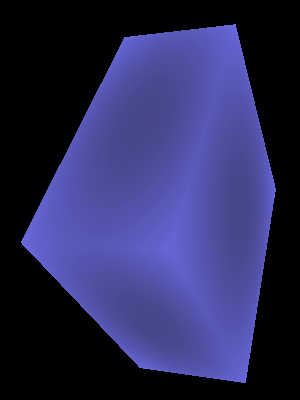
\includegraphics[width=0.5\textwidth]{pictures/Raycasting1.png}
		\subcaption{}
		\label{RaycastingExample1}
	\end{subfigure}
	\hfill
	\begin{subfigure}{0.49\textwidth}
		\centering
		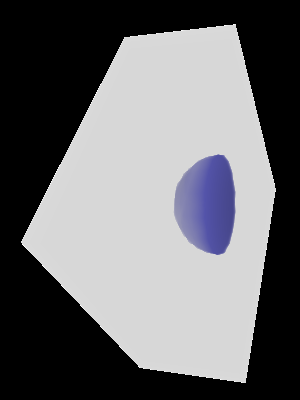
\includegraphics[width=0.5\textwidth]{pictures/Raycasting2.png}
		\subcaption{}
		\label{RaycastingExample2}
	\end{subfigure}
	\hspace*{\fill}
	\caption{Ergebnisse des Raycastings auf einem quaderf\"ormigen Feld von $3\times3$ Matrizen. In (a) werden alle Voxel des Feldes in Blau angezeigt, in (b) nur ein kleiner, halbkugelf\"ormiger Teilbereich. Zu beachten ist, dass in (a) die Farben von Punkten n\"aher am Zentrum des Feldes dunkler und in (b) die ausgeblendeten Bereiche als stark transparent und wei{\ss} dargestellt werden.}
	\label{RaycastingExample}
\end{figure}

\begin{algorithm}[t]
	\KwData{$s$ Strahlvektor der L\"ange 1, $t$ Schrittweite,\\
		$T$ 3D Textur, $p_0$ erster Abtastpunkt, $B$ ausgew\"ahlter Invariantenbereich}
	\KwResult{akkumulierte Farbe entlang des Strahls}
	$transparenz\gets$ 1,0\;
	$fragmentfarbe\gets$ (0; 0; 0; 0)\;
	\For{$i \gets 0$ \KwTo $n$}{
		\If{$transparenz < grenzwert$}{$break$\;}
		$invarianten \gets invarianten(T, p)$\;
		$dichte \gets dichte(T, p)$\; 
		\tcp{Nur im Objekt}
		\If{$invarianten \notin B$}{
			$fragmentFarbe \gets$ (1,0; 1,0; 1,0; 0,05)\;
			$transparenz \gets transparenz -$ 0,05\;
			$continue$\;
		} 
		\tcp{Nur im Invariantenraum}
		\If{$p \notin B$}{$continue$\;} 
		$voxelFarbe \gets transferfkt(dichte)$\;
		$fragmentFarbe \gets fragmentFarbe + voxelFarbe \cdot transparenz$\;
		$transparenz \gets transparenz - voxelFarbe.transparenz$\;
	}
	\vspace{0.5cm}
	\caption{Die Berechnung der akkumulierten Farbe eines Strahls durch die 3D Textur.}
	\label{RaycastingAlgorithm}
\end{algorithm}

Wenn beim Rendering des Feldes im Invariantenraum ein Abtastpunkt au{\ss}erhalb der ausgew\"ahlten Intervalle von Invarianten liegt, werden die Farbe und Dichte als 0 angenommen. Wenn dagegen beim Rendern des Objekts ein Abtastpunkt die Invarianten der Tensoren an diesem Punkt au{\ss}erhalb des Intervalls liegen, wird ein stark transparentes Wei{\ss} als Farbe festgelegt. Dadurch entsteht ein Schemen des restlichen Objektes, wodurch die Position und Form der noch sichtbaren Bereiche besser einsch\"atzbar wird. Dieser Effekt ist in \cref{RaycastingExample} zu sehen. 

Um die Tiefenwahrnehmung zu verbessern, werden zus\"atzlich Farben an Punkten, die n\"aher am Zentrum des Objekts liegen, als dunkler angezeigt, als die an weiter vom Zentrum entfernten Punkten (siehe \cref{RaycastingExample1}). Dadurch sind L\"ocher im Volumen leichter zu erkennen, ohne Lichtquellen und Schattenbildung berechnen zu m\"ussen.

\cref{RaycastingAlgorithm} beschreibt die Funktionsweise des Raycasting Algorithmus f\"ur das DVR im Orts- und Invariantenraum. Teile des Algorithmus, gekennzeichnet durch Kommentare, werden dabei ausschlie{\ss}lich in einem der beiden R\"aume ausgef\"uhrt. Die Implementierung basiert auf dem FAnToM Algorithmus \glq Volume Renderer GLSL\grq{}, ver\"andert diesen jedoch deutlich um mehrere 3D Texturen in x-Richtung als Eingabe zuzulassen, Bereiche des Volume Rendering ausblenden zu k\"onnen, korrekte \"Uberlappung mit dahinter gezeichneten Objekten sicherzustellen, die in \cref{Options} beschriebenen Optionen zu erm\"oglichen und die ben\"otigte Rechenzeit zu verk\"urzen.

\subsection{Die Interaktionswidgets}
\label{sec:Widget}
Um in der Darstellung des Feldes im Invariantenraum Intervalle von Invarianten ausw\"ahlen zu k\"onnen, wurden Interaktionfl\"achen implementiert. Leiner et al. \cite{leiner1997entwicklung} stellen an solche Elemente, die sie als \glq 3D Widgets\grq{} bezeichnen, eine Reihe von Kriterien:

\paragraph{1. Klare Erkennbarkeit der Widgets}
Widgets m\"ussen leicht als solche erkennbar sein. Unter anderem m\"ussen sie sich eindeutig von dem nicht-interaktiven Teil der Visualisierung unterscheiden lassen. Dies kann durch die Form, die Farbe oder die Positionierung der Widgets geschehen.

\paragraph{2. Zerlegung in Handles}
Da Tastatur und Maus oft nicht gen\"ugend Freiheitsgrade bieten um dreidimensionale Interaktionen direkt durch sie umsetzen zu k\"onnen, wird die Interaktion in Teile zerlegt. F\"ur jeden Teil sollte eine Komponente des Widgets reserviert werden, der durch Maus und Tastatur manipuliert werden kann. Diese Komponenten werden von Leiner et al. als \glq Handles\grq{} bezeichnet. Die Interaktion mit einem Widget gliedert sich damit in zwei Teile: Die Selektion des gew\"unschten Handles und die Manipulation des Handles.

\paragraph{3. Hervorhebung des selektierten Handles}
Damit der Benutzer sicher sein kann, das korrekte Handle selektiert zu haben, sollte dieses visuell hervorgehoben werden.

Preim et al. \cite[S.~340]{preim2015interaktive} f\"ugen noch ein weiteres Kriterium hinzu:

\paragraph{4. Affordances der Handles}
Mit dem Begriff \glq Affordances\grq{} beschreiben Preim et al. \cite[S.~137]{preim2010interaktive} Eigenschaften von Objekten, die auf die Interaktionsm\"oglichkeiten dieser Objekte hinweisen. Beispielsweise sollte ein Stuhl Affordances besitzen, die darauf schlie{\ss}en lassen, dass es m\"oglich ist, sich auf diesen zu setzen. Welche Eigenschaften als Affordances erkannt werden, h\"angt von einer Vielzahl von physikalischen und logischen Faktoren ab, sowie davon, welche anderen Interaktionen der Benutzer bereits kennt.

Da in der Literatur kein f\"ur die gew\"unschten Interaktionen geeignetes Widget beschrieben ist, wurden im Rahmen dieser Arbeit eigene Widgets entwickelt, durch die Intervalle von einer oder mehreren der drei Invarianten eines Invariantensatzes im Invariantenraum ausgew\"ahlt werden k\"onnen. Da die Invariantenr\"aume entweder zylindrische oder kartesische Koordinaten besitzt, werden f\"ur beide Koordinatensysteme jeweils eigene Widgets enwickelt. Die Auswahl des angezeigten Widgets muss dabei der Benutzer treffen, da FAnToM keine M\"oglichkeit unterst\"utzt, das verwendete Koordinatensystem abzuspeichern.

Beide Widgets kombinieren die Konzepte des Cutaways \cite[S.~406~f.]{preim2015interaktive}, einer Interaktion, bei der Teile des Datensatzes ausgeblendet werden um das Innere des Datensatzes zu zeigen, mit den Interaktionen zur Positionierung von Schnittebenen, wie sie auch in \cref{sec:Slicing} beschrieben werden. 

An die Interaktionen wurde eine weitere Anforderung gestellt. Die Interaktionen sollten so implementiert werden, dass die Auswirkung einer Interaktion mit so kurzer Verz\"ogerung wie m\"oglich angezeigt wird. Die Implementierung der Auswirkungen der Interaktionen ist deshalb innerhalb des Raycastings umgesetzt. Tats\"achlich wird die Laufzeit durch Interaktion mit dem quaderf\"ormigen Interaktionswidget generell und durch Interaktion mit der ersten Invariante beim zylindrischen Interaktionswidget reduziert, da die Bounding Box kleiner und damit die L\"ange des Schnitts zwischen Sichtstrahlen und Bounding Box geringer wird.

\subsubsection{quaderf\"ormiges Interaktionswidget}

\begin{figure}
	\centering
	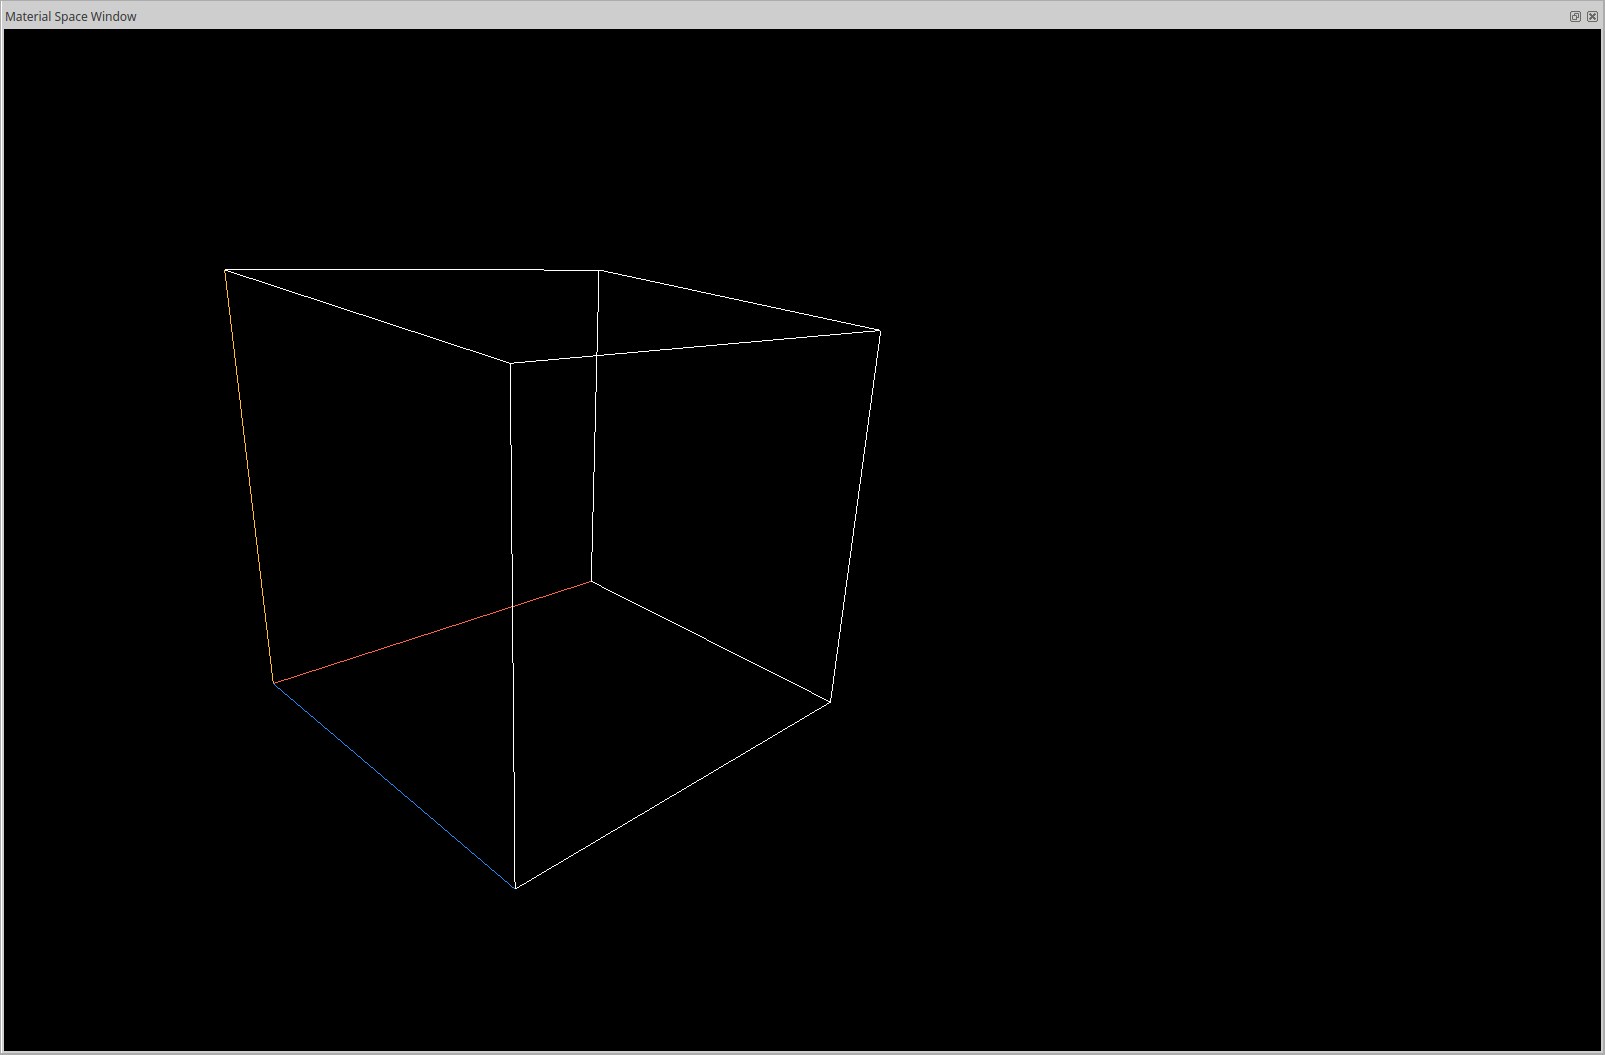
\includegraphics[width=0.55\textwidth]{pictures/QuadricInteractions.png}
	\caption{Eine Darstellung des quaderf\"ormigen Interaktionswidgets. Die drei eingef\"arbten Kanten schneiden sich in dem Punkt, dessen Koordinaten die Minima aller drei Invarianten sind. Die Farben dienen der Orientierung im Raum und weisen darauf hin, zu welcher Achse die jeweilige Kante parallel ist: Rot zur x-, Gelb zur y- und Blau zur z-Achse.}
	\label{CubicalInteractions}
\end{figure}

Das erste Interaktionswidget hat die Form eines Quaders, der das erzeugte DVR vollst\"andig umfasst. Die Seitenfl\"achen sind parallel zu paarweise aus den kartesischen Koordinatenachsen gebildeten Ebenen (xy-, xz-, yz-Ebene) und vollst\"andig transparent. Nur die Kanten des Quaders sind sichtbar, sie werden durch Linien dargestellt. Um die Orientierung des Quaders im dreidimensionalen Raum erkennbar zu machen, sind die drei Kanten, die zum Knoten links unten hinten zusammenlaufen, eingef\"arbt: Die Kante parallel zur x-Achse in rot, die Kante parallel zur y-Achse in gelb und die Kante parallel zur z-Achse in blau. Die Farben wurden so gew\"ahlt, dass sie auch bei Farbenblindheit noch unterscheidbar sind. Die Koordinaten des Schnittpunkts der drei farbigen Kanten entsprechen den Minima der einzelnen Invarianten: Die x- dem der ersten, die y- dem der zweiten und die z-Koordinaten dem der dritten Invariante. Entsprechend verlaufen die farbigen Kanten von diesem Schnittpunkt aus in Richtung der steigenden Invarianten: Die rote in Richtung der ersten, die gelbe in Richtung der zweiten und die blaue Kante in Richtung der dritten Invariante. Die Positionen der Seitenfl\"achen entsprechen im Ausgangszustand den Minima und Maxima der einzelnen Invarianten. 

Die Geraden unterscheiden sich deutlich von der Darstellung des DVR, wodurch \textbf{Kriterium~1} erf\"ullt wird. Ein Problem kann jedoch auftreten, wenn die Farben der Transferfunktion sich mit denen der Kanten \"uberschneiden. \cref{CubicalInteractions} zeigt das quaderf\"ormige Interaktionswidget.

Die Interaktion findet statt, indem eine Seitenfl\"ache durch Klicken und Halten der mittleren Maustasten ausgew\"ahlt und durch Bewegung der Maus entlang der zur Fl\"ache orthogonalen Achse verschoben wird. Jede Seitenfl\"ache stellt einen Handle dar, durch den das Minimum oder Maximum des angezeigten Intervalls einer einzelnen Invariante eingestellt wird. Dadurch ist \textbf{Kriterium 2} erf\"ullt. Die Position der Seitenfl\"achen folgt dabei der Maus, sodass immer die aktuellen Intervallgrenzen gezeigt werden. Dies erf\"ullt \textbf{Kriterium 3} zum Teil: Das aktuelle Handle liegt immer unter dem Mauszeiger und bewegt sich mit ihm, wodurch das ausgew\"ahlte Handle in der Regel erkennbar ist. 

\textbf{Kriterium 4} ist ebenfalls nur teilweise erf\"ullt. Das quaderf\"ormige Interaktionswidget kann als Teilmenge des kartesischen dreidimensionalen Raums aufgefasst werden, dessen Seitenfl\"achen bewegt werden k\"onnen. Dies stellt eine Affordance dar. Jedoch muss davon ausgegangen werden, dass diese Affordance nicht ausreicht, um Benutzer auf die m\"oglichen Interaktionen mit den Handles hinzuweisen. 

Ob und wie die Widgets ver\"andert werden k\"onnen, um die Kriterien besser zu erf\"ullen, ist Teil der weiteren Forschung und wird sich insbesondere aus Tests mit Anwendern ergeben.

Das quaderf\"ormige Interaktionswidget kann f\"ur jeden Invariantensatz verwendet werden, ist jedoch besonders f\"ur solche geeignet, bei denen alle drei Invarianten beliebige Werte in $\mathbb{R}$ annehmen k\"onnen, z.B. Eigenwerte sowie I- und J-Invariantens\"atze.

Die Berechnung, ob ein Mausklick eine Handle trifft, geschieht mittels \glq Ray-Picking\grq{}. Dabei wird, \"ahnlich wie beim Raycasting, ein Strahl ausgehend von der Kamera durch die Szene berechnet. Wenn der Strahl ein Handle trifft, wird die jeweilige Intervallschranke ausgew\"ahlt.  Wenn mehr als ein Handle getroffen wird, wird das zur Kamera n\"aheste Handle bevorzugt. Preim et al. vergleichen diese Art der Auswahl von Widgets als Metapher zum Zeigen auf ein Objekt mit einem Laserpointer oder dem Greifen eines Objekts mit der Hand \cite[344]{preim2015interaktive}.

Um die vom Interaktionswidget ausgeblendeten Bereiche besser einsch\"atzen zu k\"onnen, existiert die Option, zus\"atzlich zu den aktuellen Positionen der Kanten des Interaktionswidgets auch deren Position im Ausgangszustand einzuzeichnen. Die Darstellung dieser Kanten wird als Gitternetz oder \glq Wireframe\grq{} bezeichnet.

\begin{figure}
	\hspace*{\fill}
	\begin{subfigure}{0.2\textwidth}
		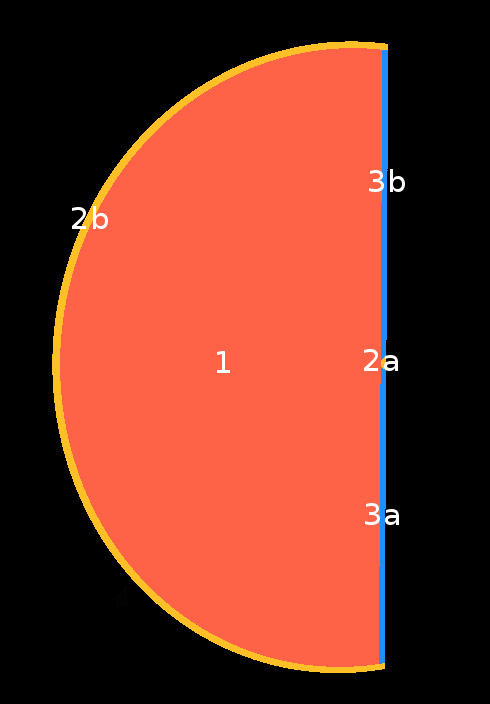
\includegraphics[width=\textwidth]{pictures/InteractionPlane.png}
		\subcaption{}
		\label{InteractionPlaneA}
	\end{subfigure}
	\hfill
	\begin{subfigure}{0.165\textwidth}
		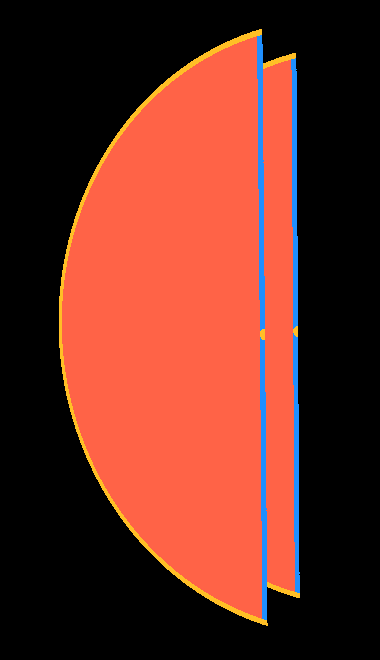
\includegraphics[width=\textwidth]{pictures/InteractionPlanes2.png}
		\subcaption{}
		\label{InteractionPlaneB}
	\end{subfigure}
	\hfill
	\begin{subfigure}{0.165\textwidth}
		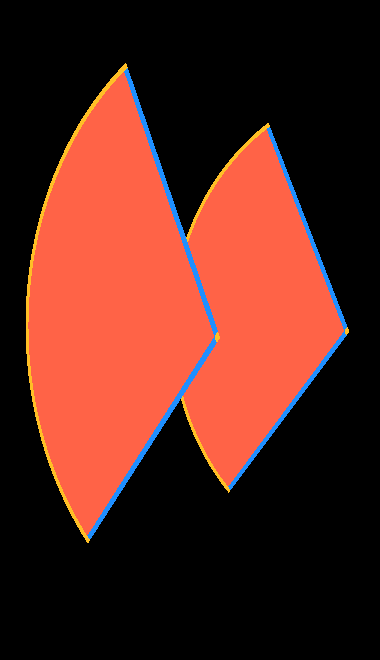
\includegraphics[width=\textwidth]{pictures/InteractionPlanes3.png}
		\subcaption{}
		\label{InteractionPlaneC}
	\end{subfigure}
	\hfill
	\begin{subfigure}{0.165\textwidth}
		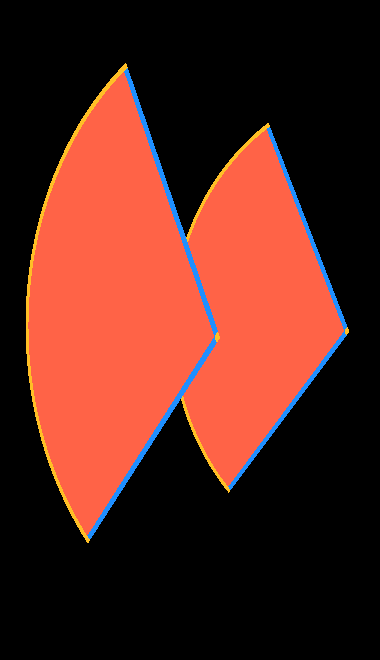
\includegraphics[width=\textwidth]{pictures/InteractionPlanes4.png}
		\subcaption{}
		\label{InteractionPlaneD}
	\end{subfigure}
	\hfill
	\begin{subfigure}{0.15\textwidth}
		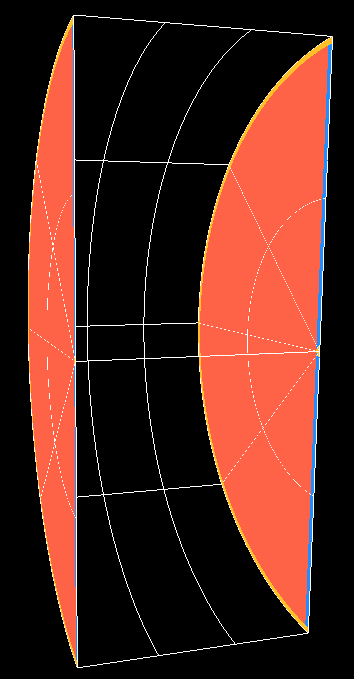
\includegraphics[width=\textwidth]{pictures/InteractionPlanes5.png}
		\subcaption{}
		\label{InteractionPlaneE}
	\end{subfigure}
	\hspace*{\fill}
	\caption{Die Darstellungen der zylindrischen Interaktionswidgets. (a) Ein Widget mit den einzelnen Handles. Ein Klick auf die Komponenten 1, 2 und 3 des Interaktionswidgets w\"ahlt das Handle der jeweils ersten, zweiten oder dritten Invariante aus. Die Komponenten 2a und 3a sind dabei die Minima der Invariante, 2b und 3b die Maxima. (b) bis (d) zeigen ver\"anderte Positionen und Formen der Interaktionswidgets durch gew\"ahlte Invariantenbereiche, wobei (b) der ersten, (c) der zweiten und (d) der dritten Invariante entspricht. In (e) ist der zylindrische Wireframe dargestellt.}
\end{figure}

\subsubsection{Zylindrisches Interaktionswidget}
Wie in \cref{sec:Invariants} beschrieben, kann es f\"ur manche Invariantens\"atze, z.B. die K- und R-Invariantens\"atze, sinnvoll sein, sie in einem zylindrischen Koordinatensystem darzustellen. Daf\"ur m\"ussen eigene Interaktionswidgets entwickelt werden, durch die, \"aquivalent zum quaderf\"ormigen Widget, die Intervallgrenzen der Invarianten manipuliert werden k\"onnen.

Die implementierten Widgets haben die Form von Kreissegmenten mit unterschiedlich eingef\"arbten Komponenten, die parallel zur yz-Ebene gezeichnet werden. Ein zylindrisches Interaktionswidget ist in \cref{InteractionPlaneA} dargestellt. Jede farbige Komponente markiert einen Teil des Widgets, durch den eine andere Invariante manipuliert werden kann. Diese Teile gliedern sich wiederum in Handles f\"ur das Minimum und Maximum der jeweiligen Invariante auf. Die Wahl der Farben folgt der gleichen Logik wie beim quaderf\"ormigen Widget. Dadurch wird \textbf{Kriterium 1} erf\"ullt.

Die Interaktion selbst ist analog zum quaderf\"ormigen Widget: Durch Klicken der Maustaste wird ein Handle ausgew\"ahlt, dessen Position der Bewegung der Maus folgt. F\"ur die erste Invariante entspricht dies der x-Koordinate des jeweiligen Widgets (siehe \cref{InteractionPlaneB}). Bei der zweiten und dritten Invariante wird die Form des Widgets angepasst: Da die zweite Invariante der Entfernung zur x-Achse entspricht, werden innerer und \"au{\ss}erer Radius des Kreissegments angepasst. Wenn der innere Radius gr\"o{\ss}er als null ist, wird somit aus dem Kreissegment ein Kreisringsektor (siehe \cref{InteractionPlaneC}). Die dritte Invariante entspricht dem Skalarprodukt zwischen der Projektion des Punktes auf die yz-Ebene und der y-Achse. Die zugeh\"origen Handles sind die beiden geraden Seiten des Kreissegments, deren Winkel zur y-Achse ver\"andert wird (siehe \cref{InteractionPlaneD}). Durch diese Aufteilung wird \textbf{Kriterium 2} erf\"ullt.

\textbf{Kriterien 3 und 4} werden genau wie beim quaderf\"ormigen Widget nur teilweise erf\"ullt und sind Thema weiterer Forschung.

Die zylindrischen Widgets stellen somit die Seitenfl\"achen eines Ausschnitts aus einem Zylinder dar, der den dargestellten Teil des Invariantenraums umfasst. Um diese Eigenschaft zu verdeutlichen, kann ein zus\"atzliches Gitter aus Linien auf der Oberfl\"ache des Zylinders gezeichnet werden, \"aquivalent zum Wireframe beim quaderf\"ormigen Interaktionswidget (siehe \cref{InteractionPlaneE}).

\subsection{Labeling}
\begin{figure}
	\centering
	\begin{subfigure}{0.6\textwidth}
		\centering
		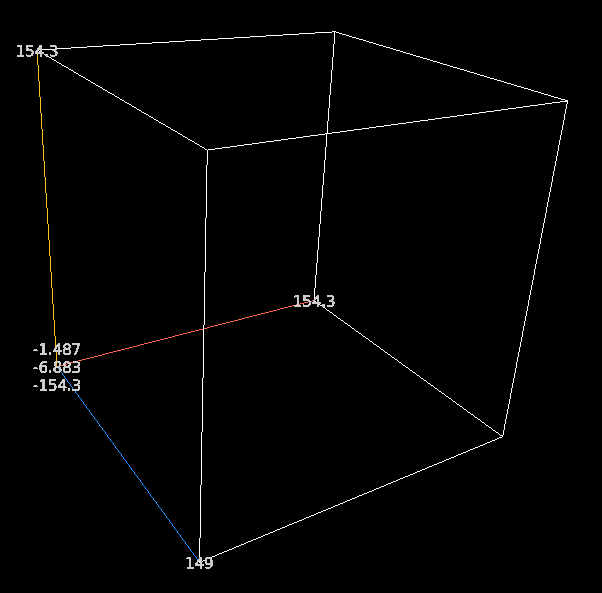
\includegraphics[height=7.cm]{pictures/QuadricLabels.png}
		\subcaption{}
		\label{QuadricLabels}
	\end{subfigure}
	\begin{subfigure}{0.3\textwidth}
		\centering
		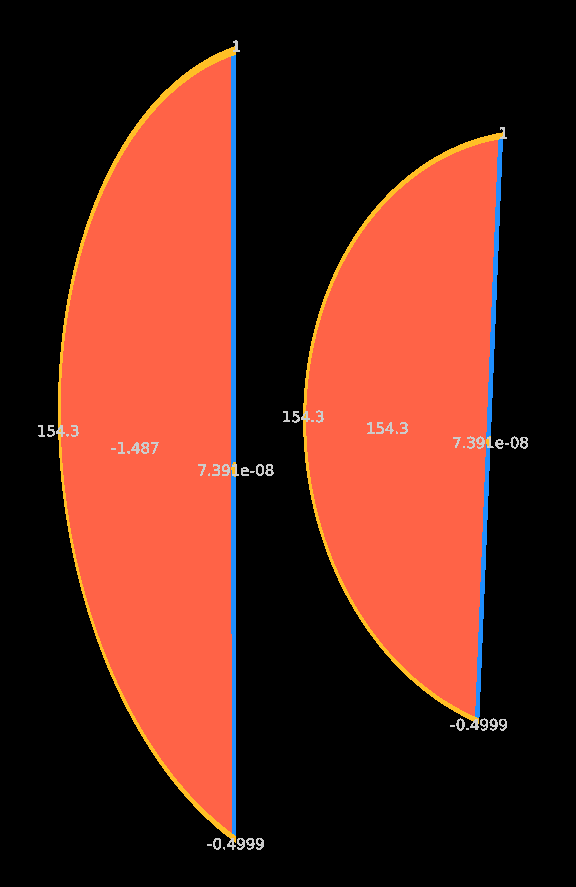
\includegraphics[height=7.3cm]{pictures/CylindricalLabels.png}
		\subcaption{}
		\label{CylindricalLabels}
	\end{subfigure}
	\caption{Labels an den Interaktionswidgets: (a) am quaderf\"ormigen Interaktionswidget, (b) an den zylindrischen Interaktionswidgets}
\end{figure}
Um die Position der Interaktionshandles im Raum ablesen zu k\"onnen, ist es m\"oglich, die eingestellten Minimal- und Maximalwerte der Invarianten an den Interaktionswidgets einzuzeichnen. Solche Beschriftungen in grafischen Oberfl\"achen werden als \glq Labels\grq{} bezeichnet.

Beim quaderf\"ormigen Interaktionswidget werden die Labels an den Endpunkten der farbigen Kanten angezeigt. An dem Punkt, an dem sich die drei Kanten schneiden, werden die Labels untereinander angeordnet, mit dem Label der ersten Invariante oben und dem der dritten unten. \cref{QuadricLabels} zeigt die Positionierung der Labels.

Die Labels am zylindrischen Interaktionswidget sind an den Handles eingezeichnet. F\"ur die erste Invariante befinden sich die Labels im Zentrum der zugeh\"origen Handles, der gro{\ss}en roten Fl\"achen. 
Auch die Labels der zweiten Invariante sind an den entsprechenden Handles, den gelben B\"ogen an der Innen- und Au{\ss}enseite der Kreisringausschnitte, eingezeichnet.
F\"ur die Position der Labels der dritten Invariante werden die \"au{\ss}eren Eckpunkte der geraden Seiten der Kreisringausschnitte gew\"ahlt. Die Positionen sind in \cref{CylindricalLabels} zu sehen.

\subsection{Weitere Interaktionen}
Es existieren noch eine Reihe weiterer Interaktionen, mit deren Hilfe die Visualisierung angepasst werden kann:
\paragraph{Rotation des DVR}
Indem die linke Maustaste gedr\"uckt und gehalten wird, kann durch die Bewegung der Maus die Visualisierung um das aktuelle Rotationszentrum gedreht werden. Die Rotation ist in Form eines sogenannten \glq Trackballs\grq{} implementiert. Preim et al. beschreiben den Trackball als imagin\"are, das Objekt umschlie{\ss}ende Kugel, die durch Mausbewegung gedreht wird und diese Bewegung auf das dargestellte Objekt, in diesem Fall das DVR und die Interaktionswidgets, \"ubertr\"agt.
\paragraph{Setzen des Rotationszentrums}
Das Rotationszentrum des Trackballs kann, wenn die zylindrischen Interaktionswidgets aktiviert sind, mittels doppeltem Linksklick an einen Punkt entlang der x-Achse gesetzt werden. Wenn dagegen das quaderf\"ormige Interaktionswidget aktiviert ist, ist das Rotationszentrum immer im Zentrum des Quaders und bewegt sich bei Einschr\"ankung der Invariantenintervallgrenzen mit.
\paragraph{Bewegung der Kameraposition}
\"Ahnlich wie bei der Rotation der Szene, kann durch Dr\"ucken und Halten der rechten Maustaste die Kameraposition mittels Bewegung der Maus innerhalb der Szene verschoben werden. 
\paragraph{Zur\"ucksetzen von Rotation und Kameraposition}
Durch Dr\"ucken der \glq c\grq{}-Taste wird die Kameraposition und die Rotation des Feldes zur\"uckgesetzt.
\paragraph{Zur\"ucksetzen der Invariantenbereiche}
Die Schranken des ausgew\"ahlten Invariantenbereichs k\"onnen durch Dr\"ucken der \glq r\grq{}-Taste zur\"uckgesetzt werden.
\paragraph{Zoomen}
Durch Drehen des Mausrades nach vorn wird die Kamera um eine Schrittl\"ange in Blickrichtung nach hinten bewegt, durch Drehen des Mausrades nach hinten eine Schrittl\"ange nach vorn. Jedes Mal wenn die Kamera auf diese Weise nach vorn bewegt wird, wird die Schrittl\"ange um einen Prozentsatz verringert, wenn die Kamera nach hinten bewegt wird um einen Prozentsatz erh\"oht. Durch diese Funktion wird eine Art von Zoomen realisiert. Die Geschwindigkeit des Zoomens reduziert sich, desto n\"aher herangezoomt wurde und beschleunigt sich, desto weiter herausgezoomt wurde. Dadurch ist es sowohl m\"oglich, auf einen bestimmten Punkt der Visualisierung heranzuzoomen als auch herauzuzoomen und sich einen \"Uberblick \"uber die Visualisierung zu verschaffen.

\subsection{Optionen des Algorithmus}
\label{Options}

Der Visualisierungsalgorithmus bietet eine Reihe von Optionen an, durch die beide DVR Darstellungen angepasst werden k\"onnen. Die Optionen gliedern sich dabei auf in solche, die f\"ur beide Darstellungen existieren und solche, die nur f\"ur eine von beiden vorhanden sind. 

\subsubsection{Gemeinsame Optionen}

\paragraph{Anzahl von Abtastpunkten}
Die Anzahl der Abtastpunkt pro Strahl kann f\"ur beide Darstellungen unabh\"angig voneinander mittels eines Textfeldes gew\"ahlt werden.

\paragraph{Jittering}
Um visuelle Artefakte zu verringern, kann durch eine Option ein pseudo-zuf\"alliger Abstand pro Strahl berechnet werden, um den der erste Abtastpunkt verschoben wird. Dadurch werden manche Artefakte, die beim Raycasting entstehen k\"onnen, vermieden.

\paragraph{Helligkeit}
Ein Schieberegler erm\"oglicht die Einstellung der Helligkeit der Farben des Volume Rendering, unabh\"angig von der Transferfunktion.

\paragraph{Dichte}
Durch einen weiteren Schieberegler kann ein Faktor festgelegt werden, mit dem die Dichte der Voxel multipliziert wird. Alternativ existiert daf\"ur auch ein Textfeld, falls exakte Werte oder Werte au{\ss}erhalb der Reichweite des Schiebereglers ben\"otigt werden.

\paragraph{Offset}
Der dritte Schieberegler legt einen Grenzwert f\"ur die Dichtewerte fest. Voxel, deren Dichte unterhalb dieses Grenzwerts liegt, werden als komplett transparent angenommen.

\paragraph{Lineare Interpolation}
Standardm\"a{\ss}ig misst die Abtastung die Dichtewerte der Textur an einem vorgegebenen Punkt. Da die Textur durch Rasterisierung entstanden ist, kann dies zu visuellen Artefakten f\"uhren, die die Darstellung \glq blockig\grq{} erscheinen lassen. Es wurde eine Option implementiert, durch die stattdessen lineare Interpolation verwendet werden kann, um die Dichte an einem Punkt zu bestimmen. Dabei wird neben der Dichte des Voxels selbst auch die Dichte der angrenzenden Voxel verwendet, und zwischen diesen der Wert am jeweiligen Abtastpunkt interpoliert.

\paragraph{Skalierung der Transparenz mit der Anzahl der Abtastpunkte im Feld}
Diese Option macht es m\"oglich, die beim Raycasting pro Pixel akkumulierte Transparenz durch die Anzahl der Abtastpunkte des Strahls zu teilen. Dies hat den Vorteil, dass stark transparente Voxel am Rand des Datensatzes deutlicher dargestellt werden, was die Erkennung von Strukturen in diesen Bereichen erleichtert, jedoch das Ablesen konkreter Dichtewerte aus der Visualisierung erschwert.

\paragraph{Anzahl der Voxel in x/y/z-Richtung}
Die Anzahl der Voxel, in die das Feld voxelisiert werden soll, kann f\"ur die einzelnen Dimensionen eingestellt werden. H\"ohere Werte f\"uhren zu einer besseren Darstellung kleiner Tetraeder, erh\"ohen jedoch die Rechenzeit und den ben\"otigten Speicher.

\subsubsection{Optionen des Objektrenderings}

\paragraph{Bounding Box}
Um die Gr\"o{\ss}e und Form des Objekts besser einsch\"atzbar zu machen, k\"onnen wei{\ss}e Linien an den Kanten der begrenzenden Fl\"achen eingezeichnet werden, also die Bounding Box der 3D Textur dargestellt werden.

\subsubsection{Optionen des Invariantenraumrenderings}
\label{sec:Options}

\paragraph{Ausgew\"ahltes Interaktionswidget}
Der Benutzer kann entscheiden, ob das quaderf\"ormige oder die zylindrischen Interaktionswidgets angezeigt werden sollen. Dies ist notwendig, da es nicht m\"oglich ist aus der internen Repr\"asentation eines Feldes in FAnToM zu bestimmen, ob dieses in zylindrischen oder kartesischen Koordinaten liegt.

\paragraph{Wireframe}
F\"ur beide Interaktionswidgets k\"onnen optional Wireframes angezeigt werden, Liniengitter an den Grenzen der Invariantenintervalle im Ausgangszustand. Die Position der Linien macht es einfacher, die ausgew\"ahlten Bereiche einzusch\"atzen. Form und Position des Wireframes sind nicht abh\"angig vom ausgew\"ahlten Invariantenbereich. Der Wireframe des zylindrischen Interaktionswidgets ist in \cref{InteractionPlaneE} zu sehen.

\paragraph{Labels einzeichnen}
Es ist m\"oglich auszuw\"ahlen, ob die Minimal- und Maximalwerte der jeweiligen Invarianten an den Widgets in Form von Labels eingezeichnet werden sollen oder nicht.

\paragraph{Interaktionswidgets ausblenden}
Da die Interaktionswidgets einen gro{\ss}en Teil des Objekts verdecken k\"onnen, besteht die M\"oglichkeit, diese auszublenden. W\"ahrend sie ausgeblendet sind, ist keine Interaktion mit ihnen m\"oglich, die Invariantenbereiche k\"onnen also nicht durch Mausinteraktion ver\"andert werden.

\paragraph{Wurzelskalierung}
Eine Fragment-Shader der Voxelisierung durchgef\"uhrte Skalierung durch Ziehen der dritten Wurzel kann an- und ausgeschaltet werden. Die Begr\"undung daf\"ur ist in \cref{sec:Raycasting} n\"aher beschrieben.

\paragraph{Normalisierung des Feldes}
\begin{figure}
	\centering
	\begin{subfigure}{0.4\textwidth}
		\centering
		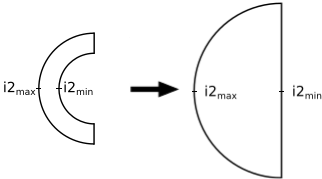
\includegraphics[height=3.5cm]{pictures/Scaling1.png}
		\subcaption{}
		\label{Scaling1}
	\end{subfigure}
	\hspace{2cm}
	\begin{subfigure}{0.4\textwidth}
		\centering
		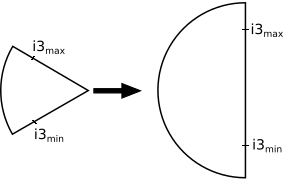
\includegraphics[height=3.5cm]{pictures/Scaling2.png}
		\subcaption{}
		\label{Scaling2}
	\end{subfigure}
	\caption{Darstellung der Normalisierung bei aktivierten zylindrischen Interaktionen: (a) Normalisierung der Darstellung der zweiten Invariante und (b) Normalisierung der dritten Invariante.}
\end{figure}

Im Invariantenraum kann das Feld beliebige Formen annehmen. Wenn beispielsweise eine Invariante nur Werte innerhalb eines sehr viel kleineren Intervalls annimmt als die anderen beiden, wird die 3D Textur als sehr flach dargestellt. Dies kann die Interpretation der Visualisierung erschweren. Deshalb ist es m\"oglich, die Darstellung des Feldes auf eine feste Form zu skalieren. Die Form ist abh\"angig davon, ob zylindrische oder quaderf\"ormige Interaktionen ausgew\"ahlt sind. Wenn das quaderf\"ormige Interaktionswidget aktiviert ist, wir die Bounding Box der 3D Textur einfach auf einen W\"urfel mit einer Kantenl\"ange von 1 skaliert. Bei aktiviertem zylindrischen Interaktionswidget dagegen wird die Darstellung des Feldes auf einen Halbzylinder mit einer H\"ohe und einem Durchmesser von 1 skaliert. Dazu wird die 3D Textur entlang der drei zylindrischen Koordinatenachsen verformt. F\"ur die erste Invariante entspricht dies einer Skalierung auf das Intervall [0;1] entlang der Mittelachse des Zylinders. Bei er zweiten Invariante wird die 3D Textur so skaliert, dass Punkte, deren zweite Invariante im Datensatz minimal ist, auf der Mittelachse des Halbzylinders und Punkte mit maximaler im Datensatz vorkommender zweiter Invariante auf der Mantelfl\"ache des Halbzylinders liegen. Eine Seitendarstellung der Skalierung der zweiten Invariante ist in \cref{Scaling1} dargestellt. \"Ahnlich geschieht auch die Skalierung der dritten Invariante. Punkte mit minimalen Werten der dritten Invariante werden so skaliert, dass sie auf der unteren H\"alfte der quadratischen Seitenfl\"ache des Halbzylinders, Punkte mit maximalen Werten so, dass sie auf der oberen H\"alfte liegen. Wiederum in einer Seitendarstellung ist dies in \cref{Scaling2} dargestellt.

\paragraph{Minimale Dichte}
Die Dichtewerte der Voxel im Invariantenraum k\"onnen sich extrem unterscheiden. Abh\"angig von der Gr\"o{\ss}e der jeweiligen Voxel traten in Testdatens\"atzen Werte zwischen $10^{-4}$ und $10^22$ auf. Damit auch Bereiche mit sehr geringer Dichte sichtbar sind, ist es m\"oglich, eine minimale Dichte im Intervall $[0;1]$ anzugeben. Wenn der in der 3D Textur abgespeicherte Wert die angegebene minimale Dichte unterschreitet, wird stattdessen dieser Wert verwendet.

\subsection{Das Intervallfenster}
\begin{figure}
	\centering
	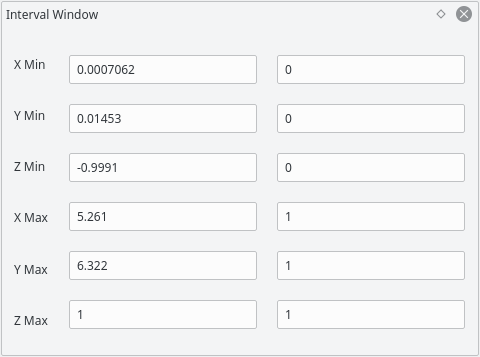
\includegraphics[width=0.4\textwidth]{pictures/IntervalWindow.png}
	\caption{Das Intervall-Fenster.}
	\label{IntervalWindow}
\end{figure}
Um die Invariantenintervalle auf exakte Werte einstellen zu k\"onnen, existiert ein weiteres Fenster (siehe \cref{IntervalWindow}). Darin sind die sechs Schranken der Invariantenintervalle tabellarisch angegeben. Das linke Textfeld gibt den absoluten, das rechte den relativen Wert im Intervall $[0;1]$ an. Alle Textfelder sind editierbar und \"Anderungen werden direkt auf die DVR angewendet.

\section{Ergebnisse}
\label{sec:Ergebnisse}
Die Visualisierung wurde auf eine Reihe von Testdatens\"atzen angewendet, um die Korrektheit und Qualit\"at der Darstellung zu bewerten. In diesem Abschnitt werden die Datens\"atze vorgestellt, die Ergebnisse der Visualisierungen gezeigt und mit bestehenden Visualisierungen verglichen sowie m\"ogliche Interpretationen erl\"autert.

Als Vergleichsdarstellung und um eine Vorstellung \"uber die Struktur der Datens\"atze zu vermitteln, werden f\"ur die ersten beiden Datens\"atze Visualisierungen der Tensoren als Ellipsoidglyphen gezeigt. Die Glyphen werden abh\"angig von den Eigenwerten des jeweiligen Tensors unterschiedlich dargestellt. Die L\"ange der Achsen eines Ellipsoids entspricht den Eigenwerten und die l\"angste Achse zeigt in Richtung des dazugeh\"origen Eigenvektors.

Die Ergebnisbilder wurden auf einem Rechner mit 8 GB Arbeitsspeicher, einem Intel i5-3570K Prozessor mit 4 Kernen und einer GeForce GTX 970 Grafikkarte in einer Aufl\"osung von 1920 $\times$ 1080 erzeugt.

Das Raycasting wurde bei allen folgenden Ergebnissen mit 5000 Abtastpunkten pro Strahl durchgef\"uhrt. Die Unterschiede in der Laufzeit des Raycastings liegen damit haupts\"achlich an der Anzahl an Pixeln, von denen aus Strahlen durch die 3D Textur geschickt werden. Die Anzahl der Pixel entspricht der Gr\"o{\ss}e der auf die Bildebene projizierten Bounding Box um die 3D Textur und \"andert sich abh\"angig von der Perspektive und der Form der Bounding Box.


\subsection{Single Point Load}

\begin{figure}
		\begin{subfigure}{0.28\textwidth}
		\centering
		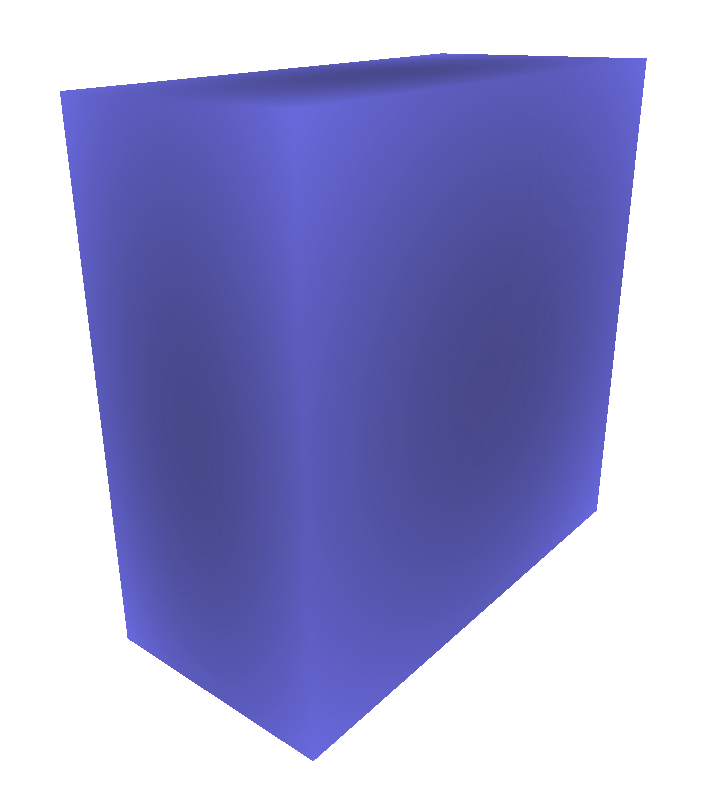
\includegraphics[height=5cm]{pictures/results/SinglePoint/SinglePoint_Object.png}
		\subcaption{}
		\label{SinglePointObject}
	\end{subfigure}
	\hspace*{\fill}
	\begin{subfigure}{0.28\textwidth}
		\centering
		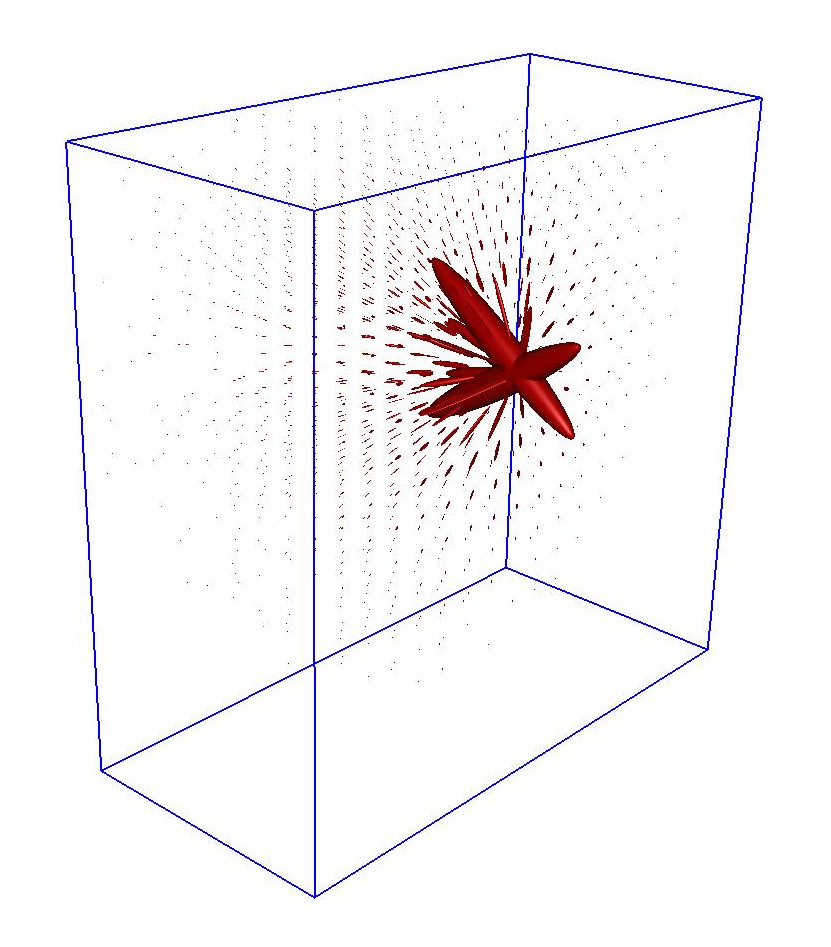
\includegraphics[height=5cm]{pictures/results/SinglePoint/SinglePoint_Ellipsoids.png}
		\subcaption{}
		\label{SinglePointEllipsoids}
	\end{subfigure}
	\hspace*{\fill}
	\begin{subfigure}{0.34\textwidth}
		\centering
		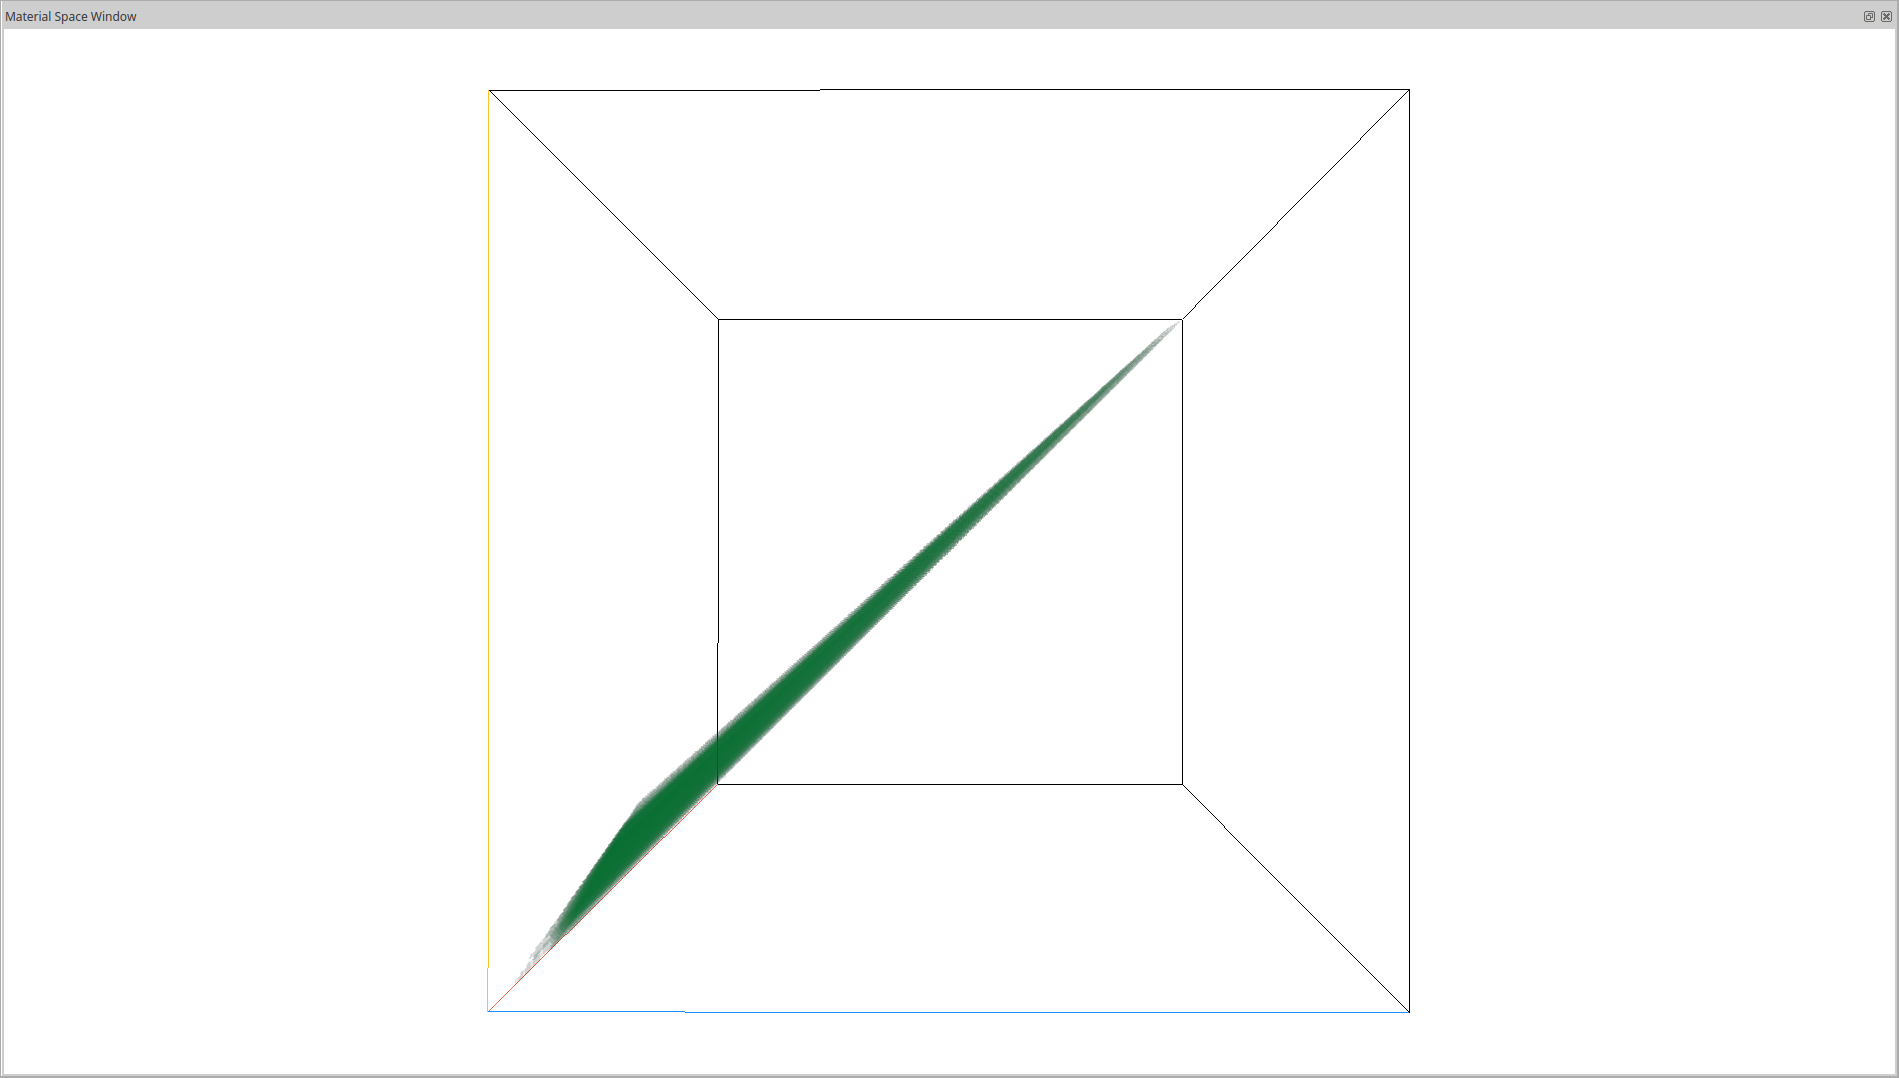
\includegraphics[height=5cm]{pictures/results/SinglePoint/SinglePoint_InvariantSpace.png}
		\subcaption{}
		\label{SinglePointInvariantSpace}
	\end{subfigure}
	\caption{Darstellung des Single Point Load Datensatzes: (a) als DVR des Objekts, (b) als Ellipsoide und (c) im Invariantenraum, berechnet mit dem I-Invariantensatz.}
	\label{SinglePoint}
\end{figure}
Um die grundlegenden Funktionen der implementierten Visualisierung zu erl\"autern, wird als erster Testdatensatz ein von FAnToM erzeugtes Tensorfeld verwendet. Dieses ist das Ergebnis einer Simulation, in der auf einen unendlichen Halbraum an einem Punkt eine Kraft einwirkt. Diese Art von Datens\"atzen wird auch als \glq Single Point Load\grq{} bezeichnet. Die entstehende mechanische Spannung wird an Punkten innerhalb des Objekts gemessen und die Tensoren in Form von $3\times3$ Matrizen gespeichert. Darstellungen des Datensatzes sind in \cref{SinglePoint} zu sehen. Der Punkt, an dem die Kraft einwirkt, befindet sich in der linken H\"alfte der vorderen, quadratischen Seite. Der Datensatz besteht aus 19.494 tetraederf\"ormigen Zellen.

Ein DVR eines quaderf\"ormigen Ausschnitts des Halbraums in der N\"ahe des Einwirkungspunktes der Kraft ist in \cref{SinglePointObject} zu sehen. Die verwendete Transferfunktion ist konstant vollst\"andig opak und blau f\"ur alle Eingabewerte, um die Form des Halbraumausschnitts deutlich darzustellen. Die Darstellung soll vor allem als Vergleichspunkt f\"ur die sp\"ater gezeigten Visualisierungen des Halbraums dienen, bei denen Teile abh\"angig von den gew\"ahlten Invarianten ausgeblendet wurden.

\cref{SinglePointEllipsoids} zeigt eine Darstellung der Tensoren als Ellipsoidglyphen. Deutlich erkennbar ist der Punkt an dem die Kraft einwirkt, denn dort sind die Glyphen am gr\"o{\ss}ten. Die Form der Ellipsoide ist l\"anglich und zeigt weg vom Einwirkungspunkt der Kraft.

F\"ur die Visualisierung wurde der I-Invariantensatz gew\"ahlt. \cref{SinglePointInvariantSpace} zeigt das DVR des Datensatzes im Invariantenraum des I-Invariantensatzes. Die Transferfunktion ordnet Bereichen hoher Dichte die Farbe Gr\"un und hohe Opazit\"atswerte zu, Bereichen geringer Dichte die Farbe Wei{\ss} und geringe Opazit\"atswerte. Da der I-Invariantensatz keiner der Invariantens\"atze ist, die sich f\"ur die Darstellung in zylindrischen Koordinaten eignen, wird ein kartesisches Koordinatensystem und das quaderf\"ormige Interaktionswidget verwendet. Auch wird die Darstellung durch Mausinteraktion um 90\textdegree~im Uhrzeigersinn um die y-Achse rotiert. Dadurch wird die Form des DVR deutlicher sichtbar. Der Punkt, an dem die drei farbigen Kanten zusammentreffen liegt nach der Drehung vorn links unten. 

Durch die Normalisierungsfunktion wurden die Dimensionen des Invariantenraumes so skaliert, dass die Intervalle der drei Invarianten gleich gro{\ss} dargestellt werden. Ohne Skalierung ist die Ausdehnung Bounding Box in Richtung der z-Achse relativ gering.

Die Form des DVR im Invariantenraum ist l\"anglich und verl\"auft entlang einer imagin\"aren Geraden zwischen zwei Punkten, die jeweils das Minimum und Maximum aller drei Invarianten darstellen. Dies zeigt eine starke lineare Abh\"angigkeit zwischen den drei Invarianten im Datensatz. Zu erkl\"aren ist dies teilweise durch die fehlende Orthogonalit\"at des I-Invariantensatzes: Desto h\"oher die Eigenwerte einer Matrix, desto h\"oher sind auch die Werte der I-Invarianten.  

Da nur f\"ur $I_1$ eine eindeutige Interpretation in der Mechanik existiert, beschr\"ankt sich die Demonstration der Funktion des Interaktionswidgets in diesem Datensatz auf $I_1$. In den \cref{SinglePointInvariant1,SinglePointInvariant2,SinglePointInvariant3} wird die untere Schranke des Intervalls der ersten Invariante erh\"oht. Im unrotierten Zustand wird dies durch die Position der linken Fl\"ache des quaderf\"ormigen Interaktionswidgets dargestellt. Da jedoch das DVR rotiert wird, ist diese Fl\"ache nun die vordere des Interaktionswidgets. Dies erschwert zwar die Interpretation, wird jedoch von der besser sichtbaren Darstellung des DVR nach der Rotation mehr als aufgewogen. Um den ausgeblendeten Bereich des DVR besser einsch\"atzen zu k\"onnen, wird das Wireframe in einem hellen Grau eingeblendet. Die \cref{SinglePointObject1,SinglePointObject2,SinglePointObject3} stellen die Bereiche des Ausschnitts des Halbraums in blau dar, in denen die Invarianten innerhalb der gew\"ahlten Intervalle liegen. Der Rest des Halbraumausschnitts wird schemenhaft in grau dargestellt.

In \cref{SinglePointInvariant1} wird das Intervall von $I_1$ um etwa 1\% verkleinert, was in der Darstellung des Invariantenraumes kaum erkennbar ist. Dennoch wird in \cref{SinglePointObject1} ein gro{\ss}er Teil des Halbraums ausgeblendet. Der minimale Wert von $I_1$ im Datensatz liegt bei 0,009, der maximale Wert bei 44,03. Aus diesen beiden Beobachtungen und der Interpretation von $I_1$ als Ma{\ss} f\"ur die St\"arke der isotropen Spannung folgt, dass in einem gro{\ss}en Teil des Datensatzes fast keine isotrope Spannung vorliegt. Nur in direkter N\"ahe zum Einwirkungspunkt der Kraft nimmt $I_1$ h\"ohere Werte an. 

\cref{SinglePointInvariant2} zeigt eine Darstellung des Invariantenraumes, in dem die untere Schranke von $I_1$ um 10\% der Intervalll\"ange erh\"oht ist. Dadurch ist die untere Spitze des DVR abgeschnitten. Die Wirkung auf die angezeigten Bereiche im DVR des Halbraums in \cref{SinglePointObject2} ist deutlich erkennbar. Diese sind im Vergleich zu \cref{SinglePointObject2} deutlich kleiner und wieder in der N\"ahe des Einwirkungspunktes der Kraft. 

Das gleiche Verhalten kann auch in \cref{SinglePointInvariant3} abgelesen werden, wo im Invariantenraum die unteren 50\% des Intervalls von $I_1$ ausgeblendet sind. \cref{SinglePointObject3} stellt die zugeh\"origen Bereiche im Halbraum dar.

Die Anzahl der erzeugten Voxel wird im Folgenden immer in der Reihenfolge x-Richtung $\times$ y-Richtung $\times$ z-Richtung angegeben.
Im Falle des Single Point Load betrug sie $400\times400\times400$ f\"ur das DVR im Invariantenraum und $400\times400\times200$ im Ortsraum. Die geringere Anzahl von Voxeln in z-Richtung des Ortsraums ist m\"oglich, da der Halbraumausschnitt in diese Richtung d\"unner ist. Dadurch wird die Gr\"o{\ss}e der 3D Textur reduziert und Speicherplatz gespart.

Die Erzeugung 3D Texturen ben\"otigte f\"ur beide DVR zusammen etwa 3 Sekunden, das Raycasting etwa 0,02 Sekunden.

\begin{figure}
	\begin{subfigure}{0.49\textwidth}
		\centering
		\includegraphics[height=4.5cm]{pictures/results/SinglePoint/SinglePoint_InvariantSpace1.png}
		\subcaption{}
		\label{SinglePointInvariant1}
	\end{subfigure}
	\hspace*{\fill}
	\begin{subfigure}{0.49\textwidth}
		\centering
		\includegraphics[height=4.5cm]{pictures/results/SinglePoint/SinglePoint_Object1.png}
		\subcaption{}
		\label{SinglePointObject1}
	\end{subfigure}
	\medskip
	\begin{subfigure}{0.49\textwidth}
		\centering
		\includegraphics[height=4.5cm]{pictures/results/SinglePoint/SinglePoint_InvariantSpace2.png}
		\subcaption{}
		\label{SinglePointInvariant2}
	\end{subfigure}
	\hspace*{\fill}
	\begin{subfigure}{0.49\textwidth}
		\centering
		\includegraphics[height=4.5cm]{pictures/results/SinglePoint/SinglePoint_Object2.png}
		\subcaption{}
		\label{SinglePointObject2}
	\end{subfigure}
	\medskip
	\begin{subfigure}{0.49\textwidth}
		\centering
		\includegraphics[height=4.5cm]{pictures/results/SinglePoint/SinglePoint_InvariantSpace3.png}
		\subcaption{}
		\label{SinglePointInvariant3}
	\end{subfigure}
	\hspace*{\fill}
	\begin{subfigure}{0.49\textwidth}
		\centering
		\includegraphics[height=4.5cm]{pictures/results/SinglePoint/SinglePoint_Object3.png}
		\subcaption{}
		\label{SinglePointObject3}
	\end{subfigure}
	\caption{Darstellungen der Interaktion mittels des quaderf\"ormigen Interaktionswidgets f\"ur den Single Point Load Datensatz. Angezeigt werden links der Invariantenraum des I-Invariantensatzes und rechts Darstellungen des Halbraumes. In (a) und (b) ist die untere Schranke um 1\% der Intervalll\"ange erh\"oht, in (c) und (d) um 10\% und in (e) und (f) um 50\%.}
	\label{SinglePointInteraction}
\end{figure}

\begin{figure}
	\hspace*{\fill}
	\begin{subfigure}{0.49\textwidth}
		\centering
		\includegraphics[height=6cm]{pictures/results/MetalDisk/MetalDisk_Object.png}
		\subcaption{}
		\label{MetalDiskObject}
	\end{subfigure}
	\begin{subfigure}{0.49\textwidth}
		\centering
		\includegraphics[height=6cm]{pictures/results/MetalDisk/strain/MetalDisk_Strain_Ellipsoids.png}
		\subcaption{}
		\label{MetalDiskStrainEllipsoids}
	\end{subfigure}
	\hspace*{\fill}
	\caption{Der Metallscheiben-Datensatz: (a) ein DVR des Objektes, (b) Tensorglyphen der mechanischen Verformung.}
	\label{MetalDisk}
\end{figure}

\subsection{Metallscheibe}

\begin{figure}
	\begin{subfigure}{0.45\textwidth}
		\centering
		\includegraphics[height=4cm]{pictures/results/MetalDisk/strain/MetalDisk_Strain_Fritzsch.png}
		\subcaption{}
		\label{MetalDiskStrainFritzsch}
	\end{subfigure}
	\begin{subfigure}{0.26\textwidth}
		\centering
		\includegraphics[height=4cm]{pictures/results/MetalDisk/strain/MetalDisk_Strain_Orthogonal.png}
		\subcaption{}
		\label{MetalDiskStrainOrthogonal}
	\end{subfigure}
	\begin{subfigure}{0.26\textwidth}
		\centering
		\includegraphics[height=4cm]{pictures/results/MetalDisk/strain/MetalDisk_Strain_Perspective.png}
		\subcaption{}
		\label{MetalDiskStrainPerspective}
	\end{subfigure}
	\caption{Darstellungen des Invariantenraums des K-Invariantensatzes f\"ur die mechanische Verformung in der Simulation der Metallscheibe: (a) Die von Fritzsch vorgestellte Visualisierung \cite[S.~45]{fritzsch2016continuousScatterplot}, (b) ein DVR mit orthogonaler Projektion in kartesischen Koordinaten, (c) ein DVR mit perspektivischer Projektion in zylindrischen Koordinaten.}
\end{figure}

Als zweites Beispiel werden die Ergebnisse einer thermo-mechanischen Simulation einer Metallscheibe verwendet. Die Simulation wurde von Prof. Dr. Thomas Nagel vom Helmholtz-Zentrum f\"ur Umweltforschung durchgef\"uhrt. Dieselben Daten bilden auch die Grundlage f\"ur ein Anwendungsbeispiel in der Arbeit von Fritzsch \cite[S.15,~45~ ff.]{fritzsch2016continuousScatterplot}. Fritzsch beschrieb die Datens\"atze dort wie folgt:

\glqq Die Metallscheibe liegt flach auf und ist entlang ihres \"au{\ss}eren Rands fixiert. Zwecks Umformung wirkt von oben ein hoher Druck ein. Zus\"atzlich wird sie von unten erw\"armt und von oben gek\"uhlt.\grqq{}\cite[S.~15]{fritzsch2016continuousScatterplot}

Die \glq obere\grq{} und \glq untere\grq{} Seite der Metallscheibe sind dabei die flachen Seiten, deren Normalen parallel zur z-Achse sind. Die z-Achse selbst zeigt nach unten. Die Anzahl der Tetraederzellen betr\"agt 26.984.

Da die Metallscheibe spiegelsymmetrisch entlang der x- und y-Achse ist, gen\"ugt es, ein Viertel der Scheibe zu simulieren. Als Ergebnisse der Simulation wurden zwei Datens\"atze erzeugt, die jeweils die mechanische Spannung und die Verformung an den Punkten der Metallscheibe enthalten. 

Beide Datens\"atze werden von Fritzsch untersucht. Dabei werden als Invarianten $I_1$ und $\sqrt{2J}$ verwendet. Da bei symmetrischen Tensoren gilt $I_1 = K_1$ und $\sqrt{2J_2} = K_2$ und die Tensoren beider Datens\"atze dreidimensional sind, ist im Folgenden stattdessen vom K-Invariantensatz die Rede. Um die Korrektheit der in der vorliegenden Arbeit implementierten Visualisierung zu zeigen und die Ergebnisse mit denen von Fritzsch vergleichen zu k\"onnen, werden Visualisierungen des K-Invariantensatzes f\"ur die mechanische Verformung erzeugt, die im Folgenden denen von Fritzsch gegen\"ubergestellt werden. F\"ur die Erstellung der DVR wird als dritte Koordinate $K_3$ verwendet.

Ein DVR der Metallscheibe ist in \cref{MetalDiskObject} in blau dargestellt. \cref{MetalDiskStrainEllipsoids} zeigt eine Darstellung der Verformungstensoren als Ellipsoidglyphen. Am inneren Rand der Scheibe, insbesondere im oberen Bereich, sind die Ellipsoide am gr\"o{\ss}ten. Dies l\"asst auf hohe Betr\"age der Eigenwerte dort schlie{\ss}en. Das Vorzeichen der Eigenwerte l\"asst sich jedoch nicht ableiten. Zum \"au{\ss}eren Rand hin nimmt die Gr\"o{\ss}e der Ellipsoide ab. Eine weitere Eigenschaft l\"asst sich aus der Form der Ellipsoide ablesen. Diese scheint am unteren Ende des Scheibenausschnitts eher l\"anglich, am oberen Ende eher rund zu sein. Scheinbar ist die Verformung am oberen Ende st\"arker isotrop als am unteren. Ebenfalls nimmt die Gr\"o{\ss}e der Ellipsoide von oben rechts nach unten links zu, die Betr\"age der Eigenwerte werden also scheinbar von unten nach oben gr\"o{\ss}er.

\cref{MetalDiskStrainFritzsch} zeigt die von Fritzsch erzeugte Visualisierung der mechanischen Verformung. Die x-Achse entspricht dem Wert von $K_1$, die y-Achse dem von $K_2$. Da seine Visualisierung ebenfalls auf den Prinzipien des Continuous Scatterplotting basiert, weisen dunklere Bereiche auf h\"ohere Dichten hin.

Damit die \"Ahnlichkeit zwischen der Darstellung von Fritzsch und den Ergebnissen der vorgestellten Arbeit deutlich werden, wurde ein DVR mit orthogonaler Projektion in kartesischen Koordinaten erzeugt, das in \cref{MetalDiskStrainOrthogonal} zu sehen ist. F\"ur die Verwendung von orthogonaler Projektion existiert im implementierten FAnToM Plugin noch keine Option, diese k\"onnte jedoch in Zukunft hinzugef\"ugt werden. Auch die verwendete Transferfunktion wurde absichtlich so gew\"ahlt, um die Darstellung des DVR an die von Fritzsch anzugleichen: Bereiche mit hoher Dichte werden als opak und schwarz dargestellt, Bereiche geringer Dichte als transparent und wei{\ss}. Die x- und y-Achsen entsprechen beim orthogonalen DVR jeweils $K_1$ und $K_2$, analog der Darstellung von Fritzsch. Die z-Achse entspricht zus\"atzlich $K_3$.

Die \cref{MetalDiskStrainFritzsch,MetalDiskStrainOrthogonal} \"ahneln sich stark, weisen jedoch eine Reihe deutlicher Unterschiede auf. Zun\"achst ist die \cref{MetalDiskStrainFritzsch} deutlich breiter, was an einer unterschiedlichen Skalierung in Richtung der x-Achse liegt. Des Weiteren ist der rechte obere Teil von \cref{MetalDiskStrainOrthogonal} deutlich heller als der von \cref{MetalDiskStrainFritzsch}. Das ist darauf zur\"uckzuf\"uhren, dass die Tetraeder in diesem Bereich sehr flach und fast parallel zur xy-Ebene sind. Dadurch werden sie nur von wenigen oder gar keiner der bei der Voxelisierung verwendeten Schnittebenen getroffen, wodurch nur wenige Voxel Dichtewerte erhalten. Durch die Skalierung der Dichte mit der Anzahl der Abtastpunkte wird der Bereich deutlich heller als in der Darstellung von Fritzsch. Ein weiterer wichtiger Faktor ist, dass das von Fritzsch implementierte Verfahren die Dichtewerte der projizierten Tetraeder einfach aufaddiert. Im DVR w\"urde dies dem R\"ontgenbildverfahren entsprechen. Da stattdessen ein transluzentes Verfahren implementiert wurde, erscheinen dichte Bereiche wie an der unteren Kante des DVR heller als dieselben Stellen in der Darstellung von Fritzsch, da helle Bereiche an der Vorderseite die dahinterliegenden Bereiche \"uberdecken.

Der K-Invariantensatz eignet sich f\"ur die Darstellung in zylindrischen Koordinaten. Daher bietet sich die mechanische Verformung der Metallscheibe an, um das zylindrische Interaktionswidget zu demonstrieren. \cref{MetalDiskStrainPerspective} zeigt ein DVR desselben Datensatzes wie \cref{MetalDiskStrainOrthogonal}, bei dem jedoch die Koordinaten der Eckpunkte der Tetraeder in Zylinderkoordinaten interpretiert wurden.

F\"ur alle vom Invariantenraum der Metallscheibe erzeugten DVR wurden die Koordinaten mit der in \ref{sec:Options} vorgestellten Option normalisiert, um die Form des Feldes im Invariantenraum besser sichtbar zu machen.

\cref{MetalDiskStrainInteraction} demonstriert die Funktionsweise des zylindrischen Interaktionswidgets. \cref{MetalDiskStrainInvariant1,MetalDiskStrainInvariant2,MetalDiskStrainInvariant3} zeigen Darstellungen der Metallscheibe im Invariantenraum. Links und rechts des DVR sind die Interaktionswidgets eingeblendet. Durch Interaktion wurden die Intervalle der anzuzeigenden Invarianten begrenzt, was durch Position und Form der Interaktionswidgets angezeigt wird. Allgemein entspricht der Teil des Invariantenraums, der innerhalb der ausgew\"ahlten Invariantenintervalle liegt, dem Bereich zwischen den roten Teilen der zylindrischen Interaktionswidgets. Teile der DVR, die au{\ss}erhalb der Intervalle liegen, werden ausgeblendet. \cref{MetalDiskStrainObject1}, \cref{MetalDiskStrainObject2,MetalDiskStrainObject3} zeigen DVR der Metallscheibe, bei denen die Bereiche mit Invarianten innerhalb des ausgew\"ahlten Intervalls in blau und au{\ss}erhalb in einem transparenten Grau dargestellt werden.

In \cref{MetalDiskStrainInvariant1} wurde das linke Interaktionswidget nach rechts bewegt, wodurch die untere Schranke des Intervalls von $K_1$ erh\"oht wurde w\"ahrend die obere Schranke gleich blieb. Die L\"ange des Intervalls wurde insgesamt um 40\% reduziert. Der Teil des DVR au{\ss}erhalb des eingeschr\"ankten Intervalls, also links vom linken Interaktionswidget, ist ausgeblendet. \cref{MetalDiskStrainObject1} zeigt das zugeh\"orige DVR im Ortsraum, in dem die Bereiche mit erster Invariante au{\ss}erhalb des eingeschr\"ankten Intervalls ausgeblendet wurden. Nur die untere H\"alfte der Metallscheibe sowie der innere Rand sind noch blau. Da $K_1$ als Ma{\ss} des isotropen Anteils der Verformungstensoren interpretiert werden kann, l\"asst sich daraus schlussfolgern, dass in diesen Bereichen starke isotrope Verformung stattfindet. Ein interessantes Detail ist, dass auf der R\"uckseite der Metallscheibe der blaue Bereich leicht gr\"o{\ss}er zu sein scheint.

\cref{MetalDiskStrainInvariant2} zeigt die Einschr\"ankung des Intervalls der zweiten Invariante. Hier ist wiederum die untere Schranke erh\"oht. Dies ist an der Form der Interaktionswidgets erkennbar. Im zylindrischen Koordinatensystem entspricht die zweite Invariante der Entfernung zur zentralen x-Achse, weshalb der ausgeblendete Bereich als halbkreisf\"ormiger wei{\ss}er Ausschnitt auf den Interaktionswidgets dargestellt ist. Dies umfasst wiederum etwa 40\% des Invariantenintervalls. Die Bereiche des Objekts, deren Invarianten im selektierten Intervall liegen, sind in \cref{MetalDiskStrainObject2} zu sehen. Sie befinden sich in einem halbkreisf\"ormigen Bereich an einer Stelle am inneren Rand der Scheibe. Aus der Interpretation von $K_2$ als Ma{\ss} f\"ur die Anisotropie l\"asst sich schlie{\ss}en, dass dort starke anisotrope Verformung stattfindet.

Zuletzt zeigt \cref{MetalDiskStrainInvariant3} die Einschr\"ankung des Intervalls der dritten Invariante. Diese entspricht in zylindrischen Koordinaten dem Winkel zur xz-Ebene. Die Einschr\"ankung wird durch die Winkel der geraden Seitenfl\"achen der Interaktionswidgets dargestellt. Die untere Schranke wird dabei um 80\% der Intervalll\"ange erh\"oht. \cref{MetalDiskStrainObject3} zeigt die Bereiche des Objekts mit hoher dritter Invariante. Diese befinden sich in einem halbkreisf\"ormigen Bereich im Inneren der Scheibe sowie entlang des gesamten inneren Randes.

Aus den Darstellungen der Invariantenbereiche im Objekt lassen sich eine Reihe von Schl\"ussen ziehen. Zun\"achst best\"atigen sich die aus der Ellipsoiddarstellung abgelesenen Informationen: Die Tensoren am inneren Rand und insbesondere im oberen Bereich des inneren Randes sind sehr viel st\"arker als im Rest der Metallscheibe. Auch, dass die Tensoren im unteren Bereich des Scheibenausschnitts st\"arker sind als im oberen stimmt \"uberein. Die zus\"atzliche Zunahme der Anisotropie von oben nach unten kann auf den gezeigten Bildern nicht abgelesen werden. Dies liegt daran, dass die Anisotropie im unteren Bereich erheblich schw\"acher ist als am inneren Rand, weshalb die Interaktion diese mit ausblendet.

Zus\"atzlich lassen sich Informationen ablesen, die die Ellipsoiddarstellung nicht bietet. Aus der Kombination aus hohem $K_2$ und $K_3$ am inneren Rand beispielsweise folgt, dass dort hohe orthotrope Anisotropie vorliegt. Interessant sind auch die leicht unterschiedlichen Verteilungen von $K_1$ auf der Vorder- und R\"uckseite der Scheibe. Dies ist wahrscheinlich auf die Temperaturunterschiede zur\"uckzuf\"uhren. 

Die erzeugten 3D Texturen bestehen aus $400\times400\times400$ Voxeln im Invariantenraum und $600\times600\times100$ Voxeln im Ortsraum. Wie schon zuvor wurde die Anzahl der Voxel im Ortsraum an die Form des Objektes angepasst, um Speicher zu sparen und die Qualit\"at des DVR zu erh\"ohen.

Die Voxelisierung zu 3D Texturen ben\"otigt insgesamt etwa 3,3 Sekunden, die Rechenzeit f\"ur ein einzelnes Bild betrug im Durchschnitt ca. 0,1 Sekunden.

\begin{figure}
	\begin{subfigure}{0.49\textwidth}
		\centering
		\includegraphics[height=4.5cm]{pictures/results/MetalDisk/strain/cylindrical/MetalDiskStrain_InvariantSpace1.png}
		\subcaption{}
		\label{MetalDiskStrainInvariant1}
	\end{subfigure}
	\hspace*{\fill}
	\begin{subfigure}{0.49\textwidth}
		\centering
		\includegraphics[height=4.5cm]{pictures/results/MetalDisk/strain/MetalDiskStrain_Object1.png}
		\subcaption{}
		\label{MetalDiskStrainObject1}
	\end{subfigure}
	\medskip
	\begin{subfigure}{0.49\textwidth}
		\centering
		\includegraphics[height=4.5cm]{pictures/results/MetalDisk/strain/cylindrical/MetalDiskStrain_InvariantSpace2.png}
		\subcaption{}
		\label{MetalDiskStrainInvariant2}
	\end{subfigure}
	\hspace*{\fill}
	\begin{subfigure}{0.49\textwidth}
		\centering
		\includegraphics[height=4.5cm]{pictures/results/MetalDisk/strain/MetalDiskStrain_Object2.png}
		\subcaption{}
		\label{MetalDiskStrainObject2}
	\end{subfigure}
	\medskip
	\begin{subfigure}{0.49\textwidth}
		\centering
		\includegraphics[height=4.5cm]{pictures/results/MetalDisk/strain/cylindrical/MetalDiskStrain_InvariantSpace3.png}
		\subcaption{}
		\label{MetalDiskStrainInvariant3}
	\end{subfigure}
	\hspace*{\fill}
	\begin{subfigure}{0.49\textwidth}
		\centering
		\includegraphics[height=4.5cm]{pictures/results/MetalDisk/strain/MetalDiskStrain_Object3.png}
		\subcaption{}
		\label{MetalDiskStrainObject3}
	\end{subfigure}
	\caption{Die Verformung des Metallscheiben-Datensatzes mit ausgew\"ahlten Invariantenbereichen. In (a) und (b) ist wurden die unteren 40\% des Intervalls von $K_1$ ausgeblendet, in (c) und (d) die unteren 40\% von $K_2$, in (e) und (f) die unteren 80\% von $K_3$.}
	\label{MetalDiskStrainInteraction}
\end{figure}

\begin{figure}
	\begin{subfigure}{0.62\textwidth}
		\centering
		\includegraphics[width=\textwidth]{pictures/results/Beam/Beam_Raith.png}
		\subcaption{}
		\label{BeamRaith}
	\end{subfigure}
	\hspace*{\fill}
	\begin{subfigure}{0.32\textwidth}
		\centering
		\includegraphics[width=\textwidth]{pictures/results/Beam/Beam_InvariantSpace.png}
		\subcaption{}
		\label{BeamInvariant}
	\end{subfigure}
	\caption{Darstellungen des Biegebalken-Datensatzes: (a) die Darstellungen von Raith et al., entnommen aus \cite{raith2019tensor}, (b) eine Darstellung als DVR im Invariantenraum}
	\label{Beam}
\end{figure}

\subsection{Biegebalken}
Die letzten zwei Testdatens\"atze stammen aus der Arbeit von Raith et al. \cite{raith2019tensor}. Der erste der beiden Datens\"atze beschreibt die Eigenwerte innerhalb eines sogenannten Biegebalkens. Raith et al. beschreiben den Biegebalken wie folgt\cite[S.~1128]{raith2019tensor}: 

Der Datensatz ist die Simulation eines waagerechten Balkens, der an einer Seite befestigt ist, w\"ahrend auf die andere Seite eine Kraft einwirkt. Generiert wurde er durch die Simulationssoftware Abaqus\cite{abaqusWebsite}. Die Dimensionen des Balkens sind 30\,mm $\times$ 30\,mm $\times$ 100\,mm. Die einwirkende Kraft betr\"agt 1000\,N und wirkt in negative y-Richtung. Der Balken besteht aus einem Metall mit einem Elastizit\"atsmodul von 210\,GPa und einer Poissonzahl von 0,3. Der Datensatz besteht aus 4320 Tetraederzellen.

Der Biegebalken wird im Folgenden immer so dargestellt, dass das befestigte Ende auf den Bildern rechts liegt und die Kraft nach unten wirkt. Als Invarianten werden die Werte der drei Hauptspannungen verwendet. Diese entsprechen den Eigenwerten der Spannungstensoren an den jeweiligen Punkten, geordnet nach ihrem Betrag. Die erste Invariante ist also stets der h\"ochste, die zweite der mittlere und die dritte der kleinste der drei Eigenwerte. Da die Tensoren symmetrisch sind und nur reelle Werte enthalten, existieren immer drei Eigenwerte.

Ziel des Tests dieses Datensatzes ist es, die Ergebnisse von Raith et al. zu reproduzieren sowie Vor- und Nachteile der erzeugten Visualisierungen mit denen von Raith et al. zu vergleichen.

In \cref{BeamRaith} ist die Visualisierung von Raith et al. abgebildet: Auf der rechten Seite werden die Positionen und Formen der Zellen des Datensatzes im Invariantenraum durch eine Wireframe-Darstellung (WF-Darstellung) angezeigt. Der transparente, rote Quader zeigt die Grenzen eines durch Interaktion ausgew\"ahlten Teils des Invariantenraumes, sehr \"ahnlich zu dem innerhalb der vorliegenden Arbeit implementierten quaderf\"ormigen Interaktionswidget. Gut sichtbar ist, dass der Quader die WF-Darstellung nur in positiver Richtung der x-Achse (roter Pfeil) und negativer Richtung der z-Achse (blauer Pfeil) schneidet. Kleine achsenparallele Sichten auf die WF-Darstellung und den Quader sind am rechten Rand abgebildet.

Die linke Seite zeigt eine WF-Darstellung, die die Zellen des Biegebalkens im Ortsraum visualisiert. Indem die Schnittfl\"achen zwischen dem Quader und den Zellen der WF-Darstellung im Invariantenraum berechnet und zur\"uck in den Ortsraum transformiert werden, entstehen die beiden gebogenen, roten Fl\"achen in der WF-Darstellung. Da die Schnittfl\"achen im Invariantenraum jeweils parallel zur xy- und yz-Ebene sind, stellen die roten Fl\"achen Isofl\"achen der ersten und zweiten Invariante dar, deren Isowerte durch die Positionen der Seitenfl\"achen des Quaders spezifiziert werden.

\cref{BeamInvariant} ist die Darstellung desselben Datensatzes im Invariantenraum als DVR. Das DVR wurde so gedreht, dass die Kameraposition und Perspektive dem der Visualisierung von Raith et al. \"ahnelt. Die unterschiedliche Form ist \"uberwiegend auf Unterschiede in der Position der Kamera und bei der Implementierung der perspektivischen Projektion zur\"uckzuf\"uhren.

Bei der Erstellung des DVR trat ein Problem auf. Sehr hohe Dichtewerte in dem Bereich, in dem sich die beiden v-f\"ormigen Komponenten im Invariantenraum treffen f\"uhrten zu Problemen mit dem Skalierungsfaktor der 3D Textur. Um die Auswirkungen auf die Visualisierung zu minimieren, verwenden wir die in \ref{sec:Options} beschriebene Option, um die minimale Dichte eines Voxels auf 5\% der maximal vorkommenden Dichte zu begrenzen. Dadurch werden Fehler minimiert und die Analyse vereinfacht. Diese Option wurde in \cref{BeamInvariant,BeamInvariant1,BeamInvariant2,BeamInvariant3} verwendet.


In dem Bereich, an dem sich die beiden v-f\"ormigen Komponenten im Invariantenraum treffen nimmt die durch die Voxelisierung berechnete Dichte im Vergleich zum Rest der 3D Textur um bis zu 20 Gr\"o{\ss}enordnungen h\"ohere Werte an. Um diese hohen Werte dennoch abspeichern zu k\"onnen, muss ein sehr hoher Skalierungsfaktor verwendet werden. Dies f\"uhrte wiederum dazu, dass die abgespeicherten Dichtewerte im Rest der 3D Textur sehr klein wurden, weshalb OpenGL sie auf 0 abrundet. Dadurch waren die v-f\"ormigen Bereiche im DVR unsichtbar. Um dies zu verhindern, wurde die in \cref{sec:Options} beschriebene Funktion zur Festlegung einer minimalen Dichte benutzt. Indem die minimale Dichte auf 5\% der maximal vorkommenden Dichte gesetzt wird, werden die v-f\"ormigen Bereiche sichtbar.


Dadurch tritt jedoch ein weiteres Problem auf: Die v-f\"ormigen Komponenten werden opaker gezeichnet als der Bereich, in dem sie zusammentreffen. Da Opakheit durch die Transferfunktion mit Werten hoher Dichte assoziiert wird, f\"uhrt dies m\"oglicherweise zu falschen Annahmen \"uber die Dichteverteilung im Invariantenraum. Tats\"achlich ist dies jedoch auf die Skalierung der Dichtewerte mit der Anzahl der Abtastpunkte pro Strahl im Raycasting zur\"uckzuf\"uhren.

Tats\"achlich liegt der Bereich, an dem die beiden v-f\"ormigen Komponenten zusammentreffen, nah am Punkt (0;0;0). Das erkl\"art auch, warum die Dichtewerte dort so hoch sind: Im Gro{\ss}teil des Biegebalkens nehmen die Eigenwerte nur sehr kleine Betr\"age an, da hier nur relativ wenig Kraft wirkt. Dadurch wird ein Gro{\ss}teil des Volumens des Biegebalkens auf diesen sehr kleinen Bereich abgebildet, was durch das Continuous Scatterplotting zu sehr hohen Dichtewerten f\"uhrt. Wie zuvor wird bei den DVR im Invariantenraum das Wireframe des quaderf\"ormigen Interaktionswidgets eingeblendet, um die Gr\"o{\ss}e der ausgeblendeten Bereiche besser einsch\"atzen zu k\"onnen.

Die von Raith et al. erzeugte Visualisierung w\"ahlt durch das von ihnen implementierte Interaktionswidget gleichzeitig eingeschr\"ankte Intervalle aller drei Invarianten aus. Es bietet sich daher an, diesen Datensatz zu nutzen, um die Funktion des gleichzeitigen Einschr\"ankens mehrerer Intervalle mithilfe des quaderf\"ormigen Interaktionswidgets zu demonstrieren. Daf\"ur ist in \cref{BeamInvariant1} die obere Schranke des gr\"o{\ss}ten Eigenwerts auf den Wert 9 festgesetzt, wie es auch in der Visualisierung von Raith et al der Fall ist. Der Wert wird im Artikel von Raith et al. nicht explizit erw\"ahnt und wurde m\"undliche nachgefragt. Im Invariantenraum entspricht dies der Bewegung der vorderen linken Seitenfl\"ache des Interaktionswidgets nach hinten rechts. Erkennbar ist, dass, wie auch bei Raith et al., die linke v-f\"ormige Komponente geschnitten und der Teil au{\ss}erhalb des Intervalls ausgeblendet wird. Der durch die Einschr\"ankung des Intervalls ausgeblendeten Bereich des Objekt DVR ist in \cref{BeamObject1} dargestellt, ein Bereich in der linken H\"alfte der oberen Kante des Balkens. Deutlich erkennbar ist die \"Ahnlichkeit der Form der Grenze zwischen dem blauen und dem grauen Bereich des DVR und dem Verlauf der oberen Invarianten-Isofl\"ache in der Visualisierung in \cref{BeamRaith}. Die von Raith et al. vorgeschlagene Erkl\"arung f\"ur Form und Position dieses Bereichs liegt in der Bedeutung der Eigenwerte bzw. Hauptspannungen. Hauptspannungen mit hohen positiven Werten weisen dabei auf Bereiche mit Zugspannungen hin, also Spannungen, die das Material in diesen Bereichen auseinanderziehen, was intuitiv im Biegebalken an dieser Stelle der Fall ist. Ein wichtiger Vorteil gegen\"uber der Visualisierung von Raith liegt darin, dass der Nutzer direkt erkennen kann, welche Bereiche innerhalb des Interaktionswidgets liegen, anstatt nur Schnittfl\"achen angezeigt zu bekommen. Besonders bei komplexen Datens\"atzen kann dies die Analyse vereinfachen.

Bei der zweiten Visualisierung, dargestellt in \cref{BeamInvariant2}, wird die untere Schranke des kleinsten Eigenwertes auf -9 festgelegt. Auch dies entspricht dem im Artikel von Raith et al. verwendeten Wert und wurde ebenfalls m\"undlich erfragt. Im Invariantenraum ist dies dargestellt durch die Bewegung der rechten vorderen Seitenfl\"ache des Interaktionswidgets nach hinten links. Wie zuvor wird dadurch eine der v-f\"ormigen Komponenten geschnitten, dieses Mal ist es jedoch die rechte. Die zugeh\"orige Darstellung der ausgeblendeten Bereiche im Objekt sind in \cref{BeamObject2} abgebildet. Es handelt sich um einen Bereich in der linken H\"alfte der unteren Kante des Balkens. Wiederum zeigt sich die \"Ahnlichkeit zu einer der Isofl\"achen in der Visualisierung von Raith et al. deutlich, dieses Mal betrifft es die untere Isofl\"ache. Die von Raith et al. vorgeschlagene Interpretation dieses Bereichs l\"asst sich auch auf die Werte der Hauptspannungen zur\"uckf\"uhren. Hauptspannungen mit negativen Werten und hohen Betr\"agen treten in Bereichen auf, in denen das Material zusammengedr\"uckt wird. Man spricht auch von Druckspannungen. Die Interpretation stimmt mit der Intuition \"uberein, dass das Material des Biegebalkens an dieser Stelle zusammengepresst wird.

\cref{BeamInvariant3} zeigt die Kombination beider zuvor erl\"auterter Intervalleinschr\"ankungen. Eine Einschr\"ankung in Richtung des mittleren Eigenwerts ist nicht notwendig, da wie schon erw\"ahnt das von Raith et al. implementierte Interaktionswidget das DVR des Biegebalkens im Invariantenraum in Richtung der y-Achse nicht schneidet. \cref{BeamObject3} zeigt die Wirkung auf das DVR im Ortsraum. Dabei wird deutlich, dass die ausgeblendeten Bereiche spiegelsymmetrisch gegen\"uber einer horizontalen Achse durch das Objekt sind. Auch dies stimmt mit den Ergebnissen von Raith et al. \"uberein.

Durch die Form des DVR im Invariantenraum bietet sich der Biegebalken-Datensatz dazu an, den explorativen Anteil der Interaktionen zu demonstrieren. Hier zeigt sich der Vorteil der implementierten Interaktionen: Bei einer Verschiebung des Interaktionswidgets wird der angezeigte Bereich im Ortsraum direkt angepasst. Im Gegensatz dazu ben\"otigten die Interakionen in der Visualisierung von Raith et al. f\"ur diesen Datensatz bereits ein vielfaches l\"anger. Zur Demonstration wurde in \cref{BeamComic} in Anhang \ref{sec:Comic} die obere Intervallgrenze schrittweise reduziert, sodass der Verlauf der Werte der ersten Invariante im DVR des Ortsraums sichtbar wird. In den ersten Schritten in \cref{BeamComic00,BeamComic05,BeamComic10,BeamComic15} vergr\"o{\ss}ert sich der im Biegebalken ausgeblendete Bereich nur langsam. Die Betr\"age der durch das Einwirken der Kraft erzeugten Spannungen nehmen scheinbar mit gr\"o{\ss}erer Entfernung zum Einwirkungspunkt stark ab. Das Wachstum des ausgeblendeten Bereichs des Biegebalkens zwischen den Abbildungen nimmt \"uber \cref{BeamComic20,BeamComic25,BeamComic30,BeamComic35,BeamComic40,BeamComic45,BeamComic50,BeamComic55,BeamComic60,BeamComic65,} hinweg zu. Wenn sich die obere Schranke der ersten Invariante jedoch an den Wert 0 ann\"ahert, zu sehen in \cref{BeamComic70,BeamComic75,BeamComic80}, wird das Wachstum wieder langsamer. Somit hat scheinbar ein erheblicher Teil des Biegebalkens eine mittelgro{\ss}e erste Invariante. Zwischen \cref{BeamComic80,BeamComic85,BeamComic90,BeamComic95} sind deutliche Spr\"unge in der Ausdehnung der ausgeblendeten Bereiche des DVR im Ortsraum zu erkennen. Da, wie schon beschrieben, in einem gro{\ss}en Teil des Biegebalkens nur sehr kleine Kr\"afte wirken, ist dieses Verhalten zu erwarten.

Interessant ist besonders der nicht ausgeblendete Bereich in \cref{BeamComic95}. Die obere Schranke der ersten Invariante hat dort einen negativen Wert. Da die erste Invariante jedoch der h\"ochsten Hauptspannung entspricht, bedeutet dies, dass dort alle drei Hauptspannungen negativ sein m\"ussen. Somit wird in einem kleinen Bereich am linken Rand des Balkens das Material aus allen Richtungen zusammengedr\"uckt.

Die erzeugten 3D Texturen hatten eine Gr\"o{\ss}e von $400\times400\times400$ im Invariantenraum und $400\times400\times800$ im Ortsraum. Das Erzeugen der 3D Texturen ben\"otigte etwa 3,1 Sekunden und die Rechenzeit f\"ur ein einzelnes Bild betrug etwa 0,05 Sekunden.

\begin{figure}
	\begin{subfigure}{0.4\textwidth}
		\centering
		\includegraphics[height=5.5cm]{pictures/results/Beam/Beam_InvariantSpace1.png}
		\subcaption{}
		\label{BeamInvariant1}
	\end{subfigure}
	\hspace*{\fill}
	\begin{subfigure}{0.4\textwidth}
		\centering
		\includegraphics[width=\textwidth]{pictures/results/Beam/Beam_Object1.png}
		\subcaption{}
		\label{BeamObject1}
	\end{subfigure}
	\medskip
	\begin{subfigure}{0.4\textwidth}
		\centering
		\includegraphics[height=5.5cm]{pictures/results/Beam/Beam_InvariantSpace2.png}
		\subcaption{}
		\label{BeamInvariant2}
	\end{subfigure}
	\hspace*{\fill}
	\begin{subfigure}{0.4\textwidth}
		\centering
		\includegraphics[width=\textwidth]{pictures/results/Beam/Beam_Object2.png}
		\subcaption{}
		\label{BeamObject2}
	\end{subfigure}
	\medskip
	\begin{subfigure}{0.4\textwidth}
		\centering
		\includegraphics[height=5.5cm]{pictures/results/Beam/Beam_InvariantSpace3.png}
		\subcaption{}
		\label{BeamInvariant3}
	\end{subfigure}
	\hspace*{\fill}
	\begin{subfigure}{0.4\textwidth}
		\centering
		\includegraphics[width=\textwidth]{pictures/results/Beam/Beam_Object3.png}
		\subcaption{}
		\label{BeamObject3}
	\end{subfigure}
	\caption{Der Biegebalken-Datensatz mit quaderf\"ormigen Interaktionen: (a) und (b) zeigen Bereiche, deren h\"ochster Eigenwert kleiner als 9 ist, (c) und (d) Bereiche in denen der kleinste Eigenwert gr\"o{\ss}er als -9 ist, (e) und (f) Bereiche in denen der gr\"o{\ss}te Eigenwert kleiner als 9 und der kleinste gr\"o{\ss}er als -9 ist}
	\label{BeamInteraction}
\end{figure}

\begin{figure}
	\begin{subfigure}{0.2\textwidth}
		\centering
		\includegraphics[width=\textwidth]{pictures/results/Nodel/Nodel_Object.png}
		\subcaption{}
		\label{NodelObject}
	\end{subfigure}
	\hspace*{\fill}
	\begin{subfigure}{0.45\textwidth}
		\centering
		\includegraphics[width=\textwidth]{pictures/results/Nodel/Nodel_Raith.png}
		\subcaption{}
		\label{NodelRaith}
	\end{subfigure}	
	\hspace*{\fill}
	\begin{subfigure}{0.3\textwidth}
		\centering
		\includegraphics[width=\textwidth]{pictures/results/Nodel/Nodel_InvariantSpace.png}
		\subcaption{}
		\label{NodelInvariant}
	\end{subfigure}
	\caption{Darstellungen des Metallkomponenten-Datensatzes: (a) ein DVR des Datensatzes im Ortsraum, (b) die von Raith et al. erzeugten Visualisierungen und (c) ein DVR des Datensatzes im Invariantenraum.}
	\label{Nodel}
\end{figure}

\subsection{Metallkomponente}
Wie auch der Biegebalken-Datensatz stammt der letzte Datensatz aus der Arbeit von Raith et al. Dort wird er wie folgt beschrieben \cite[S.~1129]{raith2019tensor}:

Der Datensatz repr\"asentiert ein aus drei Komponenten zusammengesetztes Werkst\"uck. Die erste Komponente ist ein Metalleinsatz, von dem drei Seitenbalken ausgehen. Der Metalleinsatz wird von der zweiten Komponente, einem Polymer, umschlossen. Das Polymer wiederum ist von Fasern durchzogen, die die dritte Komponente bilden. Der Datensatz ist eine Simulation, die mithilfe von Abaqus\cite{abaqusWebsite} und Helios\cite{heliosWebsite} erstellt wurde. Da das Werkst\"uck symmetrisch entlang einer Schnittfl\"ache parallel zur yz-Ebene ist, wurde nur die rechte H\"alfte simuliert. Um Fehler durch die Halbierung zu verhindern, wurden entlang der Schnittfl\"ache spezielle symmetrische Bedingungen simuliert. An der oberen und rechten Kante wird das Werkst\"uck als fixiert angenommen, w\"ahrend an der unteren Kante des Metalleinsatzes eine Kraft von 3000 N in negative y-Richtung einwirkt. Durch die Form und das Material der Komponenten sowie das spezielle Verhalten an der Schnittfl\"ache ist das Verhalten des Werkst\"ucks unter Krafteinwirkung erheblich komplexer und schwieriger zu verstehen als in den vorherigen Beispielen, was auch zu einer komplexeren Form des Datensatzes im Invariantenraum f\"uhrt. 

Die verwendeten Invarianten sind wieder die Werte der Hauptspannungen, geordnet nach ihrer Gr\"o{\ss}e.

Dieser Datensatz wurde aus mehreren Gr\"unden ausgew\"ahlt. Erstens ist er deutlich komplexer als die bisher vorgestellten Datens\"atze. Diese Komplexit\"at stellt h\"ohere Anforderungen an die Visualisierung, wie sie auch bei realen Anwendungen auftreten w\"urden. Zweitens enth\"alt der Datensatz mit 2.541.049 Tetraederzellen deutlich mehr Zellen als die anderen vorgestellten Datens\"atze. Und drittens existiert mit der Arbeit von Raith et al. ein Referenzpunkt, mit dem die erzeugten Ergebnisse verglichen werden k\"onnen.

In \cref{Nodel} sind Visualisierungen des Metallkomponenten-Datensatzes abgebildet. \linebreak \cref{NodelObject} zeigt ein DVR des Objekts. Unten links ist die H\"alfte des Metalleinsatzes mit seinen drei Seitenbalken zu erkennen. \cref{NodelRaith} zeigt die von Raith et al. erzeugten Visualisierungen. Wie auch beim Biegebalken-Datensatz werden die Zellen durch eine WF-Darstellung visualisiert. Auf der rechten Seite ist die WF-Darstellung im Invariantenraum zu sehen. Interessant dabei ist, dass das Koordinatensystem linksh\"andig ist, also x- und y-Achse vertauscht sind. Ein kleiner Bereich des Invariantenraumes ist ausgew\"ahlt, dargestellt durch das rote, quaderf\"ormige Interaktionswidget. 

Im linken Teil von \cref{NodelRaith} ist die WF-Darstellung des Objekts zu sehen. Die Schnittfl\"achen zwischen den Seitenfl\"achen des Quaders und den Zellen der WF-Darstellung im Invariantenraum wurden zur\"uck in den Ortsraum transformiert und sind in rot eingezeichnet. Der dadurch markierte Bereich wird von Raith et al. als eine Region beschrieben, in der \"ublicherweise Besch\"adigungen im Material auftreten.

\cref{NodelInvariant} zeigt den Datensatz als DVR im Invariantenraum. Das in dieser Arbeit implementierte DVR-Verfahren verwendet ein rechtsh\"andiges Koordinatensystem. Um die \"Ahnlichkeit zum rechten Teil von \cref{NodelRaith}, der in linksh\"andigen Koordinaten erzeugt wurde, zu erh\"ohen, wurde \cref{NodelInvariant} vertikal gespiegelt. 

Wegen der Komplexit\"at des Datensatzes ist es ohne gr\"undliche Kenntnisse der physikalischen Prozesse schwierig, Informationen aus der Form des DVR im Invariantenraum oder aus den Formen der ein- und ausgeblendeten Teile des DVR im Ortsraum zu ziehen. Die vorliegende Arbeit beschr\"ankt sich daher darauf, die von Raith et al. erzeugten Visualisierungen zu reproduzieren und zu vergleichen.

\cref{NodelInteractions} zeigt den Metallkomponenten-Datensatz, in dem die Intervalle aller drei Invarianten eingeschr\"ankt wurden. 
Durch Interaktion mit dem quaderf\"ormigen Interaktionswidget wurden die oberen und unteren Schranken aller Invariantenintervalle eingeschr\"ankt. Dies ist in \cref{NodelInvariant1} dargestellt. Der ausgew\"ahlte Bereich zeigt gro{\ss}e \"Ahnlichkeit zu der Form und Position des Interaktionswidgets in der Visualisierung von Raith et al. in \cref{NodelRaith}. Der Bereich im Ortsraum, in dem Invarianten innerhalb des gew\"ahlten Intervalls auftreten, ist in \cref{NodelObject1} dargestellt: Ein kleiner Bereich am oberen Rand der Metallkomponente. Dieser entspricht in Form und Position den Ergebnissen von Raith et al., wie sie in \cref{NodelRaith} zu sehen sind.

\begin{figure}
	\begin{subfigure}{0.49\textwidth}
		\centering
		\includegraphics[height=4.5cm]{pictures/results/Nodel/Nodel_InvariantSpace1.png}
		\subcaption{}
		\label{NodelInvariant1}
	\end{subfigure}
	\hspace*{\fill}
	\begin{subfigure}{0.49\textwidth}
		\centering
		\includegraphics[height=4.5cm]{pictures/results/Nodel/Nodel_Object1.png}
		\subcaption{}
		\label{NodelObject1}
	\end{subfigure}
	\caption{Der Metallkomponenten-Datensatz, eingeschr\"ankt auf einen kleinen quaderf\"ormigen Bereich mit hohen Werten der ersten und zweiten sowie mittleren Werten der dritten Invariante: (a) Darstellung im Invariantenraum und (b) Darstellung im Ortsraum.}
	\label{NodelInteractions}
\end{figure}

Die 3D Textur des Invariantenraumes besteht aus $400\times400\times200$ Voxeln, die des Ortsraums aus $600\times600\times100$ Voxeln. Die Berechnung der 3D Texturen ben\"otigte insgesamt ca. 30 Sekunden, was auf die sehr viel gr\"o{\ss}ere Anzahl an Tetreaedern in diesem Datensatz zur\"uckzuf\"uhren ist. Um ein einzelnes Bild zu erzeugen wurden durchschnittlich ca. 0,08 Sekunden ben\"otigt.

\subsection{Fazit der Ergebnisse}
Die implementierte Visualisierung wurde anhand der vorgestellten Beispiele demonstriert. 

Es konnte gezeigt werden, dass die gleichzeitige Darstellung eines Datensatzes im Orts- und Invariantenraum es erm\"oglicht, aus der Position eines Punktes im Invariantenraum Informationen \"uber den an diesem Punkt definierten Tensor im Ortsraum zu ziehen. Auch die Form des Feldes im Invariantenraum kann interessante Einblicke in die Struktur des Feldes bieten. Da die Invarianten dom\"anenspezifische Eigenschaften der Tensoren repr\"asentieren, ist es somit m\"oglich, Bereichen der Objekte Eigenschaften zuzuordnen. Die Kernaufgabe der Visualisierung, Informationen \"uber die Struktur von Tensorfeldern zu vermitteln, ist somit erf\"ullt. Die Korrektheit der Visualisierung wurde durch Vergleich mit der Arbeit von Fritzsch und Raith et al. nachgewiesen.

Zus\"atzlich konnte gezeigt werden, dass die vorgestellte Visualisierung einige Vorteile gegen\"uber anderen Tensorfeldvisualisierungen bietet. Verglichen mit der Darstellung durch Ellipsoidglyphen wurde deutlich, dass es in der implementierten Visualisierung durch die Interaktionen deutlich einfacher war Eigenschaften der Tensoren und ihre Position im Objekt abzulesen. Auch kleine Ver\"anderungen, wie die unterschiedlichen Spannungen an Vorder- und R\"uckseite der Metallscheibe, die bei der Ellipsoidglyphendarstellung nicht erkennbar waren, wurden sichtbar dargestellt.

Die Verbesserungen gegen\"uber der Arbeit von Fritzsch liegen in der gleichzeitigen Darstellung aller drei Invarianten und den implementierten Interaktionen. Dadurch wurde die Interpretierbarkeit der Darstellung stark erh\"oht. Im Vergleich mit der Visualisierung von Raith et al. konnten die Vorteile der Darstellung als DVR und der k\"urzeren Rechenzeit der Interaktionen gezeigt werden. W\"ahrend bei Raith et al. die Visualisierung ca 3,0 Sekunden ben\"otigt, um den Effekt einer Interaktion darzustellen, geschieht dies in der von uns implementierten Visualisierung in weniger als 0,1 Sekunden. Dadurch wird die explorative Analyse des Datensatzes m\"oglich.

Wie f\"ur alle vorgestellten Datens\"atze gezeigt werden konnte, stellt die Repr\"asentation von Tensoren durch Invarianten eine sinnvolle Reduktion der Datenmenge pro Tensor dar. \textbf{Herausforderung 1} ist somit erf\"ullt. Dadurch, dass die Invarianten abh\"angig von der Dom\"ane des Datensatzes ausgew\"ahlt werden k\"onnen sind ebenfalls \textbf{Herausforderungen 3 und 4} gel\"ost. Dies wird besonders deutlich, wenn man die Visualisierungen des Metallscheiben Datensatzes mit dem des Biegebalkens vergleicht. Dort ver\"anderte sich die Interpretation der Visualisierung durch die Wahl unterschiedlicher Invariantens\"atze stark.

Die \textbf{Herausforderung 2} kann nur als teilweise gel\"ost betrachtet werden. Zwar konnte am Beispiel des Metallkomponenten-Datensatzes gezeigt werden, dass auch Datens\"atze mit mehreren Millionen Tensoren dargestellt und durch Interaktionen in akzeptabler Zeit manipuliert werden k\"onnen. Die Voxelisierung skaliert jedoch schlecht mit der Anzahl an Tetraedern, sowohl in Hinblick auf Laufzeit als auch auf die Erkennbarkeit der Form einzelner Tetraeder. Insbesondere extrem hohe Dichtewerte durch \"Uberlappung von Tetraedern stellen ein Problem dar, wie am Beispiel des Biegebalkens gezeigt wurde. Die verwendete L\"osung manipuliert die Dichtewerte im Datensatz so stark, dass die Visualisierung einen falschen Eindruck der Dichteverteilung im Invariantenraum vermittelt.

Auch die implementierten Interaktionen wurden ausf\"uhrlich demonstriert. Es haben sich zwei unterschiedliche Anwendungsf\"alle f\"ur die Interaktionen ergeben. Der erste Fall, demonstriert im Biegebalken- und Metallkomponenten-Datensatz, besteht darin, einen spezifischen Bereich im Invariantenraum auszuw\"ahlen und die zugeh\"origen Bereiche im Ortsraum zu betrachten. Dazu muss der Nutzer die spezifischen Bereiche des Invariantenraumes bereits kennen oder aus der Form des DVR im Invariantenraum ablesen k\"onnen. Wenn dies nicht gegeben ist, k\"onnen die Interaktionen nur f\"ur den zweiten Anwendungsfall verwendet werden. Dieser entspricht der explorativen Analyse des Datensatzes durch Interaktion. Durch die Interaktionen werden beliebige Intervalle von Invarianten ausgew\"ahlt und angezeigt. Indem die Form und Verteilung der Invarianten interpretiert wird, kommt es zu einem Gewinn an Informationen. Dies wurde im Single Point Load-, Metallscheiben- und Biegebalken-Datensatz demonstriert. Ein Sonderfall der explorativen Analyse ist beim Biegebalken Datensatz dargestellt. Indem der Ortsraum betrachtet wird w\"ahrend die Invariantenintervalle schrittweise eingeschr\"ankt werden, werden Informationen \"uber die Verteilung der Invarianten innerhalb des Objekts gewonnen. Insgesamt konnte gezeigt werden, dass die implementierten Interaktionen dabei helfen \textbf{Herausforderungen 2 und 3} zu l\"osen.

Obwohl die Interpretation der Form des Feldes im Invariantenraum noch immer ein Problem darstellt, konnte beim Biegebalken- und Metallkomponenten-Datensatz gezeigt werden, dass sichtbare Strukturen im Invariantenraum Bereichen mit interessanten Eigenschaften im Ortsraum entsprechen.

\section{Ausblick}
\label{sec:Ausblick}
Die Ergebnisse wurden Experten f\"ur Kontinuumsmechanik von der Technischen Universit\"at Dortmund und dem Helmholtz-Zentrum f\"ur Umweltforschung vorgef\"uhrt, wobei die Reaktionen positiv waren. Es wurde jedoch kritisiert, dass die explorative Analyse intensive Kenntnisse der Datens\"atze voraussetzt. In der Praxis werden sogenannte Materialmodelle eingesetzt, die das Verhalten von Materialien beschreiben. Ausgehend davon lassen sich Invariantenbereiche definieren. Diese sind jedoch nicht immer zylinderachsenparallel oder quaderf\"ormig wie die bereits implementierten Interaktionswidgets. Dies w\"are z.B. bei einem Material der Fall, das bei h\"oheren isotropen Spannungen auch h\"ohere anisotrope Spannungen aush\"alt. Ein solches Materialmodell w\"urde im K-Invariantenraum die Form eines Kegels annehmen. 

Das Laden von Materialmodellen und Ausw\"ahlen der entsprechenden Bereiche k\"onnte eine lohnenswerte Erweiterung des Systems darstellen. Die Interpretation durch den Nutzer w\"urde erleichtert, da er die Bereiche nicht mehr per Hand einstellen m\"usste und daher weniger Kenntnisse \"uber die Invarianten und ihre Bedeutung notwendig w\"aren. Gleichzeitig w\"aren die Ergebnisse exakter und besser in der Praxis anwendbar. Dadurch w\"urden \textbf{Herausforderungen 3 und 4} besser gel\"ost werden. 

Ein weiterer Ansatzpunkt f\"ur Verbesserungen w\"are das Voxelisierungsverfahren. Da die Voxelisierung f\"ur einen Gro{\ss}teil der Rechenzeit der Visualisierung verantwortlich ist, w\"urden Optimierungen dort die Gesamtlaufzeit deutlich reduzieren. Dadurch w\"are es auch m\"oglich, die Masseerhaltung durch Supersampling zu implementieren, ohne die ben\"otigte Zeit zu stark zu erh\"ohen. Auch Probleme wie d\"unne, ebenenparallele Bereiche k\"onnten durch Verbesserungen der Voxelisierung behoben werden, genauso wie Verfahren zur Reduktion der Treppeneffekte. \textbf{Herausforderung 2} k\"onnte durch diese Verbesserungen wirksamer bearbeitet werden als es im Moment der Fall ist.

Wie in den Vergleichen mit den Ergebnissen von Fritzsch erw\"ahnt ist die Implementierung einer Option zum Umschalten auf orthogonale Projektion im DVR eine m\"oglicherweise lohnenswerte Erweiterung. Dadurch w\"urde das Ablesen von Koordinaten aus der Visualisierung erleichtert werden. Auch Optionen zur Erstellung von R\"ontgenbildern, MIPs oder Isofl\"achen sind vorstellbar.

Ebenfalls vorstellbar ist die Verwendung eines alternativen DVR-Verfahrens, um Probleme der Voxelisierung komplett zu umgehen. Eine M\"oglichkeit daf\"ur k\"onnte eine stark modifizierte Cell Projection sein. Dadurch w\"urde sich jedoch wahrscheinlich die f\"ur Interaktion ben\"otigte Rechenzeit deutlich erh\"ohen.

Zuletzt bieten auch die Interaktionswidgets Raum f\"ur Weiterentwicklung, besonders in Hinblick auf Affordances, Hervorhebung der Handles bei Selektion und der visuellen Abhebung der Widgets von den DVRs.
 
Weitere Verbesserungsm\"oglichkeiten werden wahrscheinlich deutlich werden, wenn das System in der Praxis eingesetzt wird. 

\section{Zusammenfassung}
\label{sec:Zusammenfassung}
Innerhalb der vorliegenden Arbeit wurde ein System entwickelt und evaluiert, das die Untersuchung von Tensorfeldern mithilfe von Invariantens\"atzen erm\"oglicht. Es wurden mathematische, physikalische und technische Grundlagen erl\"autert und verschiedene DVR-Verfahren in Hinblick auf die Problemstellung verglichen. Ein Verfahren zur Erstellung dreidimensionaler Continuous Scatterplots wurde vollst\"andig implementiert. Ebenfalls wurde ein Raycasting-Algorithmus implementiert, um die erzeugten dreidimensionalen Continuous Scatterplot darzustellen. Mithilfe von Interaktionen konnten die Zusammenhänge zwischen dem Invarianten- und dem Ortsraum dargestellt werden. Eine Vielzahl weiterer Interaktionen und Optionen, die es Nutzern erm\"oglichen, die Visualisierung an ihre Bed\"urfnisse anzupassen, wurden ebenfalls realisiert und vorgestellt. Zum Abschluss wurde die Visualisierung auf vier Datens\"atze angewendet, die Ergebnisse pr\"asentiert und mit denen anderer Tensorfeldvisualisierungen verglichen. Dabei konnten die Ergebnisse der anderen Visualisierungen reproduziert und Vorteile der Visualisierung demonstriert werden. Anwendungsf\"alle f\"ur die Interaktionen und ihr Nutzen zur Analyse der vorgestellten Datens\"atze wurde gezeigt. Jedoch wurden auch Nachteile und Probleme des Verfahrens sichtbar, von denen ein Teil durch k\"unftige Arbeit behoben werden k\"onnte. Die in der Einleitung gestellten Herausforderungen konnten zum Gro{\ss}teil zufriedenstellend gel\"ost werden.

% %%%%%%%%%%%%%%%%%%%%%%%%%%%%%%%%%%%%%%%%%%%%%%%%%%%%%%%%%%%%%%
% HERE ENDS YOUR DOCUMENT
% %%%%%%%%%%%%%%%%%%%%%%%%%%%%%%%%%%%%%%%%%%%%%%%%%%%%%%%%%%%%%%

% Settings for the references (which are numbered in roman style)
\label{LastPageBeforeRefs}
\clearpage
\ofoot{\vspace{-0.1cm}\textbf{\large\thepage}/\textbf{\large\getpagerefnumber{LastAppendixPage}}}
\pagenumbering{Roman}

\printbibliography
\label{LastBibPage}
\clearpage
\section{Anhang}
\subsection{Anhang A}
\label{sec:Comic}
\begin{figure}[!htb]
	\begin{subfigure}{\textwidth}
		\centering
		\raisebox{-0.5\height}{\includegraphics[width=0.21\textwidth]{pictures/results/Beam/comic/Beam_InvariantSpace_00.png}}
		\hspace{1cm}
		\raisebox{-0.5\height}{\includegraphics[width=0.32\textwidth]{pictures/results/Beam/comic/Beam_Object_00.png}}
		\subcaption{0\%}
		\label{BeamComic00}
	\end{subfigure}
	\medskip
	\begin{subfigure}{\textwidth}
		\centering
		\raisebox{-0.5\height}{\includegraphics[width=0.21\textwidth]{pictures/results/Beam/comic/Beam_InvariantSpace_05.png}}
		\hspace{1cm}
		\raisebox{-0.5\height}{\includegraphics[width=0.32\textwidth]{pictures/results/Beam/comic/Beam_Object_05.png}}
		\subcaption{5\%}
		\label{BeamComic05}
	\end{subfigure}
	\medskip
	\begin{subfigure}{\textwidth}
		\centering
		\raisebox{-0.5\height}{\includegraphics[width=0.21\textwidth]{pictures/results/Beam/comic/Beam_InvariantSpace_10.png}}
		\hspace{1cm}
		\raisebox{-0.5\height}{\includegraphics[width=0.32\textwidth]{pictures/results/Beam/comic/Beam_Object_10.png}}
		\subcaption{10\%}
		\label{BeamComic10}
	\end{subfigure}
	\medskip
	\begin{subfigure}{\textwidth}
		\centering
		\raisebox{-0.5\height}{\includegraphics[width=0.21\textwidth]{pictures/results/Beam/comic/Beam_InvariantSpace_15.png}}
		\hspace{1cm}
		\raisebox{-0.5\height}{\includegraphics[width=0.32\textwidth]{pictures/results/Beam/comic/Beam_Object_15.png}}
		\subcaption{15\%}
		\label{BeamComic15}
	\end{subfigure}
	\caption{Darstellungen des Biegebalken Datensatzes. Die obere Schranke des gr\"o{\ss}ten Eigenwerts wurde jeweils um den angegebenen Prozentsatz der gesamten Intervalll\"ange verringert.}
\end{figure}

\begin{figure}
	
	\ContinuedFloat
	
	\begin{subfigure}{\textwidth}
		\centering
		\raisebox{-0.5\height}{\includegraphics[width=0.21\textwidth]{pictures/results/Beam/comic/Beam_InvariantSpace_20.png}}
		\hspace{1cm}
		\raisebox{-0.5\height}{\includegraphics[width=0.32\textwidth]{pictures/results/Beam/comic/Beam_Object_20.png}}
		\subcaption{20\%}
		\label{BeamComic20}
	\end{subfigure}
	\medskip
	\begin{subfigure}{\textwidth}
		\centering
		\raisebox{-0.5\height}{\includegraphics[width=0.21\textwidth]{pictures/results/Beam/comic/Beam_InvariantSpace_25.png}}
		\hspace{1cm}
		\raisebox{-0.5\height}{\includegraphics[width=0.32\textwidth]{pictures/results/Beam/comic/Beam_Object_25.png}}
		\subcaption{25\%}
		\label{BeamComic25}
	\end{subfigure}
	\medskip
	\begin{subfigure}{\textwidth}
		\centering
		\raisebox{-0.5\height}{\includegraphics[width=0.21\textwidth]{pictures/results/Beam/comic/Beam_InvariantSpace_30.png}}
		\hspace{1cm}
		\raisebox{-0.5\height}{\includegraphics[width=0.32\textwidth]{pictures/results/Beam/comic/Beam_Object_30.png}}
		\subcaption{30\%}
		\label{BeamComic30}
	\end{subfigure}
	\medskip
	\begin{subfigure}{\textwidth}
		\centering
		\raisebox{-0.5\height}{\includegraphics[width=0.21\textwidth]{pictures/results/Beam/comic/Beam_InvariantSpace_35.png}}
		\hspace{1cm}
		\raisebox{-0.5\height}{\includegraphics[width=0.32\textwidth]{pictures/results/Beam/comic/Beam_Object_35.png}}
		\subcaption{35\%}
		\label{BeamComic35}
	\end{subfigure}
	\caption{Darstellungen des Biegebalken Datensatzes. Die obere Schranke des gr\"o{\ss}ten Eigenwerts wurde jeweils um den angegebenen Prozentsatz der gesamten Intervalll\"ange verringert.}
\end{figure}

\begin{figure}
	
	\ContinuedFloat

	\begin{subfigure}{\textwidth}
		\centering
		\raisebox{-0.5\height}{\includegraphics[width=0.21\textwidth]{pictures/results/Beam/comic/Beam_InvariantSpace_40.png}}
		\hspace{1cm}
		\raisebox{-0.5\height}{\includegraphics[width=0.32\textwidth]{pictures/results/Beam/comic/Beam_Object_40.png}}
		\subcaption{40\%}
		\label{BeamComic40}
	\end{subfigure}
	\medskip
	\begin{subfigure}{\textwidth}
		\centering
		\raisebox{-0.5\height}{\includegraphics[width=0.21\textwidth]{pictures/results/Beam/comic/Beam_InvariantSpace_45.png}}
		\hspace{1cm}
		\raisebox{-0.5\height}{\includegraphics[width=0.32\textwidth]{pictures/results/Beam/comic/Beam_Object_45.png}}
		\subcaption{45\%}
		\label{BeamComic45}
	\end{subfigure}
	\medskip
	\begin{subfigure}{\textwidth}
		\centering
		\raisebox{-0.5\height}{\includegraphics[width=0.21\textwidth]{pictures/results/Beam/comic/Beam_InvariantSpace_50.png}}
		\hspace{1cm}
		\raisebox{-0.5\height}{\includegraphics[width=0.32\textwidth]{pictures/results/Beam/comic/Beam_Object_50.png}}
		\subcaption{50\%}
		\label{BeamComic50}
	\end{subfigure}
	\medskip
	\begin{subfigure}{\textwidth}
		\centering
		\raisebox{-0.5\height}{\includegraphics[width=0.21\textwidth]{pictures/results/Beam/comic/Beam_InvariantSpace_55.png}}
		\hspace{1cm}
		\raisebox{-0.5\height}{\includegraphics[width=0.32\textwidth]{pictures/results/Beam/comic/Beam_Object_55.png}}
		\subcaption{55\%}
		\label{BeamComic55}
	\end{subfigure}
	\caption{Darstellungen des Biegebalken Datensatzes. Die obere Schranke des gr\"o{\ss}ten Eigenwerts wurde jeweils um den angegebenen Prozentsatz der gesamten Intervalll\"ange verringert.}
\end{figure}

\begin{figure}
	
	\ContinuedFloat
	
	\begin{subfigure}{\textwidth}
		\centering
		\raisebox{-0.5\height}{\includegraphics[width=0.21\textwidth]{pictures/results/Beam/comic/Beam_InvariantSpace_60.png}}
		\hspace{1cm}
		\raisebox{-0.5\height}{\includegraphics[width=0.32\textwidth]{pictures/results/Beam/comic/Beam_Object_60.png}}
		\subcaption{60\%}
		\label{BeamComic60}
	\end{subfigure}
	\medskip
	\begin{subfigure}{\textwidth}
		\centering
		\raisebox{-0.5\height}{\includegraphics[width=0.21\textwidth]{pictures/results/Beam/comic/Beam_InvariantSpace_65.png}}
		\hspace{1cm}
		\raisebox{-0.5\height}{\includegraphics[width=0.32\textwidth]{pictures/results/Beam/comic/Beam_Object_65.png}}
		\subcaption{65\%}
		\label{BeamComic65}
	\end{subfigure}
	\medskip
	\begin{subfigure}{\textwidth}
		\centering
		\raisebox{-0.5\height}{\includegraphics[width=0.21\textwidth]{pictures/results/Beam/comic/Beam_InvariantSpace_70.png}}
		\hspace{1cm}
		\raisebox{-0.5\height}{\includegraphics[width=0.32\textwidth]{pictures/results/Beam/comic/Beam_Object_70.png}}
		\subcaption{70\%}
		\label{BeamComic70}
	\end{subfigure}
	\medskip
	\begin{subfigure}{\textwidth}
		\centering
		\raisebox{-0.5\height}{\includegraphics[width=0.21\textwidth]{pictures/results/Beam/comic/Beam_InvariantSpace_75.png}}
		\hspace{1cm}
		\raisebox{-0.5\height}{\includegraphics[width=0.32\textwidth]{pictures/results/Beam/comic/Beam_Object_75.png}}
		\subcaption{75\%}
		\label{BeamComic75}
	\end{subfigure}
	\caption{Darstellungen des Biegebalken Datensatzes. Die obere Schranke des gr\"o{\ss}ten Eigenwerts wurde jeweils um den angegebenen Prozentsatz der gesamten Intervalll\"ange verringert.}
\end{figure}

\begin{figure}
	
	\ContinuedFloat
	
	\begin{subfigure}{\textwidth}
		\centering
		\raisebox{-0.5\height}{\includegraphics[width=0.21\textwidth]{pictures/results/Beam/comic/Beam_InvariantSpace_80.png}}
		\hspace{1cm}
		\raisebox{-0.5\height}{\includegraphics[width=0.32\textwidth]{pictures/results/Beam/comic/Beam_Object_80.png}}
		\subcaption{80\%}
		\label{BeamComic80}
	\end{subfigure}
	\medskip
	\begin{subfigure}{\textwidth}
		\centering
		\raisebox{-0.5\height}{\includegraphics[width=0.21\textwidth]{pictures/results/Beam/comic/Beam_InvariantSpace_85.png}}
		\hspace{1cm}
		\raisebox{-0.5\height}{\includegraphics[width=0.32\textwidth]{pictures/results/Beam/comic/Beam_Object_85.png}}
		\subcaption{85\%}
		\label{BeamComic85}
	\end{subfigure}
	\medskip
	\begin{subfigure}{\textwidth}
		\centering
		\raisebox{-0.5\height}{\includegraphics[width=0.21\textwidth]{pictures/results/Beam/comic/Beam_InvariantSpace_90.png}}
		\hspace{1cm}
		\raisebox{-0.5\height}{\includegraphics[width=0.32\textwidth]{pictures/results/Beam/comic/Beam_Object_90.png}}
		\subcaption{90\%}
		\label{BeamComic90}
	\end{subfigure}
	\medskip
	\begin{subfigure}{\textwidth}
		\centering
		\raisebox{-0.5\height}{\includegraphics[width=0.21\textwidth]{pictures/results/Beam/comic/Beam_InvariantSpace_95.png}}
		\hspace{1cm}
		\raisebox{-0.5\height}{\includegraphics[width=0.32\textwidth]{pictures/results/Beam/comic/Beam_Object_95.png}}
		\subcaption{95\%}
		\label{BeamComic95}
	\end{subfigure}
	\caption{Darstellungen des Biegebalken Datensatzes. Die obere Schranke des gr\"o{\ss}ten Eigenwerts wurde jeweils um den angegebenen Prozentsatz der gesamten Intervalll\"ange verringert.}
	\label{BeamComic}
\end{figure}
\clearpage

\label{LastAppendixPage}
\end{document}
